\documentclass[a4paper]{book}
%\documentclass[twosided]{book}
% for < > 

\usepackage[T1]{fontenc}
\usepackage[pdftex]{graphicx}
\usepackage{fancyvrb} % Verbatim border
\usepackage{alltt}
\usepackage{acronym}
\usepackage{pdfpages}

% For text highlight
\usepackage{minted}

% break URLs
%\usepackage[breaklinks=true]{hyperref}
%\usepackage{breakurl}

% colors
\usepackage{color}
\definecolor{light-gray}{gray}{0.95}
\definecolor{medium-gray}{gray}{0.75}

% header 
\usepackage{fancyhdr}
\pagestyle{fancy}
\renewcommand{\chaptermark}[1]%
{\markboth{\MakeUppercase{\thechapter.\ #1}}{}}
\renewcommand{\sectionmark}[1]%
{\markright{\MakeUppercase{\thesection.\ #1}}}
\renewcommand{\headrule}{{\color{medium-gray}%
\hrule width\headwidth height\headrulewidth \vskip-\headrulewidth}}
\renewcommand{\headrulewidth}{0.5pt}
\renewcommand{\footrulewidth}{0pt}
\newcommand{\helv}{%
\fontfamily{phv}\fontsize{9}{11}\selectfont}
\fancyhf{}
\fancyhead[LE,RO]{\helv \thepage}
\fancyhead[LO]{\helv \rightmark}
\fancyhead[RE]{\helv \leftmark}

% example class
\usepackage{float}
\floatstyle{plain}
\newfloat{example}{thp}{loe}
\floatname{example}{Example}

% French
\usepackage[utf8]{inputenc}
%\usepackage[frenchb]{babel}

% ---
% Change the background colour of the algorithm floats.
\usepackage{listings}

\begin{document}
\sloppy
\thispagestyle{empty}
\pagestyle{empty}
\includepdf{page-garde_fr}

~\\
\newpage
\includepdf{page-garde_en}

\thispagestyle{empty}
\pagestyle{empty}

\chapter*{Acknowledgement}
\thispagestyle{empty}
\pagestyle{empty}
First, I would like to express my deepest gratitude to my thesis supervisor, Professor Maryline Laurent, for her guidance throughout my thesis, for all the fruitful discussions that we had, and especially for her patience. Her wide knowledge and her logical way of thinking have been of great value for me. I would also like to thank her for being attentive towards me and providing me with invaluable encouragements when I was lost and could not find my way.\\

My gratitude goes to Sir Tim Berners-Lee for having invited me to work under his guidance at MIT, as well as for his incredible work which inspired me to pursue this thesis.\\

I am very thankful to Olivier Berger, research engineer in the Informatics Department of TELECOM SudParis, for our extensive collaboration and for accepting to be member of the examination jury.\\

Many thanks go towards my colleagues and friends, from TELECOM SudParis and beyond, which supported me during all these years. Among them I would like to mention Aymen Boudguiga and Collins Mtita, with whom I have shared more than just an office.\\

I would finally like to thank my family for their continuous love and support. A special thank you goes to my wife Raluca for her love and constant support, for all the late nights and early mornings, and for keeping me sane over the past few months. Thank you for everything, but most of all, thank you for being my best friend. I owe you everything.\\

This work has been funded entirely by TELECOM SudParis, member of group Institut Mines-TELECOM.

% abstract
\chapter*{Abstract}
\thispagestyle{empty}
\pagestyle{empty}
Ensuring personal data ownership and interoperability for decentralized social Web applications is currently a debated topic, especially when taking into consideration the aspects of privacy and access control. Since the user's data are such an important asset of the current business models for most social Websites, companies have no incentive to share data among each other or to offer users real ownership of their own data in terms of control and transparency of data usage. We have concluded therefore that it is important to improve the social Web in such a way that it allows for viable business models while still being able to provide increased data ownership and data interoperability compared to the current situation.\\

To this regard, we have focused our research on three different topics: identity, authentication and access control. First, we tackle the subject of decentralized identity by proposing a new Web standard called \textit{Web Identity and Discovery} (WebID), which offers a simple and universal identification mechanism that is distributed and openly extensible. Next, we move to the topic of authentication where we propose WebID-TLS, a decentralized authentication protocol that enables secure, efficient and user friendly authentication on the Web by allowing people to login using client certificates and without relying on Certification Authorities. We also extend the WebID-TLS protocol, offering delegated authentication and access delegation. Finally we present our last contribution, the Social Access Control Service, which serves to protect the privacy of Linked Data resources generated by users (e.g. profile data, wall posts, conversations, etc.) by applying two social metrics: the \textit{social proximity distance} and \textit{social contexts}.

\newpage
~
\newpage

\clearpage
\pagenumbering{roman}
\tableofcontents

\pagestyle{fancy}

% Acronyms
\chapter*{List of acronyms}
\label{ch:acronyms}
\markboth{\MakeUppercase{List of acronyms}}{}

\begin{acronym}
\acro{AC}{Access Condition}
\acro{ACL}{Access Control List}
\acro{AEC}{Access Evaluation Context}
\acro{AIR}{Accountability in RDF}
\acro{API}{Application Programming Interfaces}
\acro{ATR}{Access Tagging Rule}
\acro{CA}{Certification Authority}
\acro{CRUD}{Create-Read-Update-Delete}
\acro{CSR}{Certification Signing Request}
\acro{DAC}{Discretionary Access Control}
\acro{DANE}{DNS-Based Authentication of Named Entities}
\acro{DN}{Distinguished Name}
\acro{DNS}{Domain Name System}
\acro{DNSSEC}{Domain Name System Security Extensions}
\acro{DNT}{Do Not Track}
\acro{DOAP}{Description of a Project}
\acro{ETag}{Entity Tags}
\acro{FOAF}{Friend-of-a-Friend}
\acro{FQDN}{Fully Qualified Domain Name}
\acro{GPG}{GNU Privacy Guard}
\acro{HTTP}{Hypertext Transfer Protocol}
\acro{HTTPS}{Hypertext Transfer Protocol Secure}
\acro{IdP}{Identity Provider}
\acro{ISP}{Internet Service Provider}
\acro{JSON}{JavaScript Object Notation}
\acro{LDP}{Linked Data Platform}
\acro{LDPC}{Linked Data Platform Containers}
\acro{LDPR}{Linked Data Platform Resource}
\acro{MAC}{Mandatory Access Control}
\acro{MIT}{Massachusetts Institute of Technology}
\acro{N3}{Notation 3}
\acro{OTP}{One-Time Password}
\acro{PIN}{Personal Identification Number}
\acro{PKI}{Public Key Infrastructure}
\acro{RBAC}{Role-based Access Control}
\acro{RDF}{Resource Description Framework}
\acro{RDFa}{Resource Description Framework in Attributes}
\acro{REST}{Representational State Transfer}
\acro{RFC}{Request for Comments}
\acro{RM}{Relationship Monitor}
\acro{RP}{Relying Party}
\acro{RSA}{Stands for Ron Rivest, Adi Shamir and Leonard Adleman, who first publicly described the cryptographic algorithm.}
\acro{RWW.I/O}{Read-Write-Web Input/Output}
\acro{S4AC}{Social Semantic SPARQL Security for Access Control}
\acro{SAC}{Static Access Control}
\acro{SACS}{Social Access Control Service}
\acro{SAML}{Security Assertion Markup Language}
\acro{SAN}{Subject Alternative Name}
\acro{SIOC}{Semantically-Interlinked Online Communities}
\acro{SP}{Service Provider}
\acro{SPARQL}{SPARQL Protocol and RDF Query Language}
\acro{SPKAC}{Signed Public Key and Challenge}
\acro{SSL}{Secure Sockets Layer}
\acro{SSWAC}{Social Semantic Web Access Control}
\acro{TAKES}{Trustful Authentication and Key Exchange System}
\acro{TLS}{Transport Layer Security}
\acro{UI}{User Interface}
\acro{URI}{Uniform Resource Identifier}
\acro{URL}{Uniform Resource Locator}
\acro{W3C}{World Wide Web Consortium}
\acro{WAC}{Web Access Control}
\acro{WebID}{Web Identity and Discovery}
\acro{XACML}{eXtensible Access Control Markup Language}





\end{acronym}

% Examples
\listof{example}{List of examples}

% Figures
\listoffigures



% Introduction / Problem 
\chapter{Introduction}
\label{ch:intro}
\setcounter{page}{1}
\pagenumbering{arabic}

\section{Problem statement and motivation}
\label{sec:statement}
Over the past decade, we have witnessed a dramatic increase in the number of social Web applications. These applications come in different forms and offer different services such as social networks, content management systems (CMS), software forges, bug trackers, blogging tools, or collaboration services in general.\\

Since the launch of the first large social networking website in 1997~\cite{ellison2007social}, the social Web has seen a significant increase in its size and usage. Rather than simply consuming websites, users began to generate their own content through blogging tools and social networks, marking the start of Web 2.0 and the Semantic Web~\cite{berners1999weaving}. Social Websites have responded to this new trend by providing users with the ability to create their own personal profile where they could list friends, post photos, status updates and more. Later, some of these websites have also provided plug-ins that were used to integrate some of their social functionalities on other third-party websites. But what exactly is a social website and what functionalities do these websites offer to users? Is the ability to form a connection between users enough to consider a website to be a part of the social Web, and how can we expect the social Web to evolve in the future?\\

In this thesis we will analyse and propose means to achieve data ownership and interoperability for decentralized social Web applications, with respect to privacy and access control. Since the user's data are such an important asset of the current business models for most social Websites, companies have no incentive to share data among each other or to offer users real ownership of their own data in terms of control and transparency of data usage. We have concluded therefore that it is important to improve the social Web in such a way that it allows for viable business models while still being able to provide increased data ownership and data interoperability compared to the current situation.\\

The following section of the introduction outlines the reasons and the motivation that has driven us to pursue this thesis. The first topic discusses the lack of control over users' data. The second topic covers identity, as a key factor for the decentralized social Web. Finally, the third topic will be an introduction to achieving interoperability on the Web.

\subsection{Data silos, losing control over our data}
\label{subsec:intro-silos}
A current practice specific to most Web services is to centralize user resources, becoming the so-called "data silos". Often when adhering to particular services we usually end up creating dedicated local accounts, which ties and limits us to a particular service and/or resource. Figure~\ref{fig:wall_garden} aptly illustrates this aspect, depicting how people's freedom within a particular social networking site is limited and how they would like to "jump out of the walled gardens" to interact with "other" social networking sites, such as to share their data with their friends who may be members of other social networking sites. Furthermore, users have no control over how their personal account data are used by applications, as it is the case for private data that is often sent to third party companies for advertising purposes.

\begin{figure}[h]
  \begin{center}
    \includegraphics[width=300px]{img/walled_garden.jpg}
        \caption{'Everywhere and nowhere', an illustration by David Simonds, 2008.}
        \label{fig:wall_garden}
  \end{center}
\end{figure}

One may argue that better privacy policies may reduce the risk of exposure. However, even if users decide to protect their public data through rigorous privacy settings, or even remove their accounts, there is no guarantee that the process is instant and more importantly, permanent. This is mainly due to the fact that countries have passed laws forcing online services to store user data for several months up to one year or an unlimited period of time.\\

Companies attempt to justify the practice of \textit{data silos} stating that they have better control over user actions while allegedly offering better security. Online businesses stand to gain a lot from data mining their users in order to be able to increase their sales, or offer targeted publicity. In most of the cases, they offer "free" sign-up for their services and provide people with numerous attractive features, encouraging them to provide additional personal data, effectively turning the users from customers into products which are often "sold" to third party advertising companies. For this matter and to the detriment of users, privacy is often found as an additional feature and it is not implemented by design.\\

While it is true that some people join public communities and disclose personal information in order to find new friends who share common interests, others would simply want to have more control over their privacy. The situation worsens when social networks force the users into providing their real names without presenting them with alternatives, like creating multiple identities or using pseudonyms.\\

A solution to the so-called \textit{data silos} can be achieved through decentralization, where users are free to host their data wherever they want. In the following section we will discuss how decentralized identity systems play an important role in achieving true data ownership for users.


\subsection{Identity, a key factor for the decentralized social Web}
\label{subsec:intro-id}
Before discussing decentralized social Web applications, we must first define the concept of \textit{identity}. The first question we ask ourselves is related to the form and nature of online identities. Often, an online identity starts with a unique identifier binding a person to a user profile describing them. The identity of a person may also include the sum of all opinions and postings that have been generated by that person, as well as relationships between the person and other people, all contributing to the one's reputation.\\

Since online identities also deal with personal data, a number of risks are related to the exposure of these data~\cite{rosenblum2007}. There have been accounts of employers who have been collecting information about potential employees from their blogs~\cite{viegas2005bloggers} and social networking sites~\cite{mannan2008privacy}, and have used this information to dismiss them or deny them jobs. A recent study~\cite{careerbuilder2009} performed by a popular career and resume-building website revealed that 46\% of executives say they are likely to make a hiring decision based on a prospective employee's online identity or Facebook profile. So far, the most common workaround for people has been to replace real identities with pseudonyms.\\

Identity is easily one of the most difficult research areas on the Web, as it requires both practical solutions and multidisciplinary research. We believe that identity implies to be able to refer reliably to anything, abstract or real, and in different contexts. In our day to day lives, we find the concept of personal identity to be quite simple (i.e. our names). Yet on closer inspection, we find that applying these concepts to a Web scale becomes quite tricky, as is the case when we type our name into a search engine and see that it may refer to many other people in different contexts. It becomes even worse when it might refer to us in a context that we did not intend to.\\

One way to deal with identity is to establish a common convention that identifies particular things in a uniform manner that is 
easily reused in diverse contexts. When applied to the Web, it becomes obvious that using HTTP Uniform Resource Identifiers (URIs) as global identifiers is the preferred choice. The key advantage of HTTP URIs over any other identification scheme (e.g. email addresses, unique user IDs, etc.) is that linked data principles say these URIs should return a useful description of what the URI identifies when accessed in a Web browser or computer application using the HTTP protocol.\\

The process of establishing one's identity leads to \textit{identification}, which is also a key component of decentralized social Web services. Having a persistent identity across different application domains is very difficult to achieve, since the concept of \textit{decentralized authentication} requires a considerable effort from large entities in terms of compatibility, as well as powerful trust relationships between all parties. Many services authenticate users based on user name and password combinations, which results in having to remember and manage a lot of accounts. In that respect, federated and decentralized authentication services like OpenID~\cite{recordon2006openid}, OAuth~\cite{hardt-d-2012-a} and Mozilla Persona~\cite{browserid} have proven to be quite useful. However, once the authentication has been performed, some services still require that users have local accounts in order to manage profile data. To this regard, WebID, the first of our contributions, provides both a decentralized identity platform, as well as the basis for a deceptively simple yet secure decentralized authentication mechanism through the use of cryptography, in the form of WebID-TLS. WebID and WebID-TLS will be presented in detail in Chapter~\ref{ch:identity}.

\subsection{Interoperability based on the Semantic Web and LDP}
\label{sec:semweb}
A decentralized Web application must be able to work \textbf{across different application domains}, enabling different applications to interact with each other through the use of data semantics. It is important that users be allowed to choose where to store their data, may that be on personal servers they own and keep in their homes, or entrusting their data to their friends or people they trust. Users may even take advantage of a myriad of cloud storage services available on the Web, though steps must be taken to ensure the privacy of their data, with respect to the service providers.\\

The main cause for which storing data in a decentralized manner is unpopular, is that major Web services have no incentive to share data among each other or to give users more ownership than necessary for their own data. Even though most applications provide Application Programming Interfaces (APIs) which are dedicated to performing specific interoperability tasks, developers are still required to have a priori knowledge of these APIs before attempting to provide interoperability. To our knowledge, there is currently no standardized API for decentralized Web applications, leaving at the discretion of each application to define its own API. Recently however, a standard is being proposed for such an API within the World Wide Web Consortium (W3C). It relies on the \textit{Semantic Web}, which refers to the Web of data~\cite{berners1999weaving}, in order to offer true interoperability.

\subsubsection{The Semantic Web}
The Semantic Web should be considered in some ways like a global database, or better yet an information space. Since most of the information on the Web is designed for human readers, though only useful for human-to-human interaction, the Semantic Web intends to allow machines to participate in this interaction by providing languages for expressing information in a machine processable form. In other words, the Semantic Web offers the tools to convey the meaning of data so that it will be understood by computers and not misinterpreted.\\

The most common means used by the Semantic Web to describe information are the Resource Description Framework (RDF)~\cite{klyne2004resource} and the Turtle~\cite{beckett2008turtle} syntax. While RDF is based upon the idea of making statements about resources (in particular Web resources) in the form of subject-predicate-object expressions (called \textit{triples}), the Turtle syntax is utilized to express data in the RDF data model.\\

A typical triple is presented in Example~\ref{ex:semweb}, where the subject is \verb+<>+ (which refers to the current document), the predicate is \verb+foaf:maker+ while the object being \verb+https://barry.example/profile#me+. All statements are contained within the same document, residing at \verb+https://barry.example/profile+, and having as \textit{primaryTopic} the inner reference \textbf{\textit{\#me}} pointing to a \textit{Person}, namely Barry. A visual representation of the same triples is provided as a graph in Figure~\ref{fig:intro-foaf}.\\

\begin{example}
\begin{minted}{turtle}
@prefix foaf: <http://xmlns.com/foaf/0.1/> .

<> a foaf:PersonalProfileDocument ;
      foaf:maker <https://barry.example/profile#me> ;
      foaf:primaryTopic <https://barry.example/profile#me> .

<#me> a foaf:Person ;
      foaf:name "Barry" ;
      foaf:knows <https://example.edu/p/Ann#MSc> ;
      foaf:weblog <http://barry.example/blog> .
\end{minted}
\caption{A typical subject-predicate-object relation in Turtle.}
\label{ex:semweb}
\end{example}

\begin{figure}[htbp]
  \begin{center}
    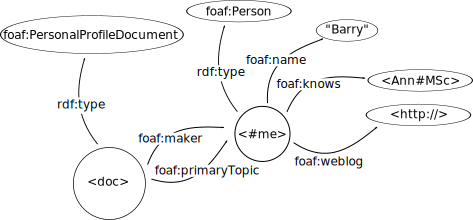
\includegraphics[width=300px]{img/foaf-ontology.pdf}
        \caption{A graph representation of Barry's profile.}
        \label{fig:intro-foaf}
  \end{center}
\end{figure}

The Semantic Web facilitates cross-domain applications and services, thanks to data being structured into ontologies and vocabularies. An ontology formally represents knowledge as a set of concepts within a domain, and the relationships between those concepts. Vocabularies are a less formal way of expressing concepts or entities and the relations between them. A typical case of a large linked data application is DBPedia\footnote{http://dbpedia.org}, which, essentially, makes the content of Wikipedia available in RDF. The importance of DBPedia is not only that it includes Wikipedia data, but also that it incorporates links to other datasets on the Web, e.g., to Geonames\footnote{http://geonames.org}. By providing extra links expressed as RDF triples, applications are able to exploit the semantics of data and gain additional knowledge from other datasets. Conversely, by virtue of integrating facts from several datasets, applications are now able to provide a better user experience.\\

\subsubsection{The Linked Data Platform}
The \textbf{Linked Data Platform} (LDP)~\cite{ldp2013} is considered to be the first attempt at producing a standardized API for Web applications. Essentially, it is a set of best practices for a read-write Linked Data architecture, based on HTTP access to Web resources that describe their state using the RDF data model. It describes the use of HTTP verbs for fetching (GET), updating (POST/PATCH), creating (PUT) and deleting (DELETE) resources from servers that expose their resources as Linked Data. It provides several rules as well as clarifications and extensions of the four rules of Linked Data, which are the following:

\begin{enumerate}
  \item Use URIs as names for entities;
  \item Use HTTP URIs so that people can look up those names;
  \item When someone looks up a URI, provide useful information, using existing standards (e.g. RDF, SPARQL);
  \item Include links to other URIs so that more information can be discovered.
\end{enumerate}

Adopting LDP is important since developers no longer have to redefine APIs every time a new Semantic Web application is created.\\

LDP focuses on two important concepts, \textbf{resources} and \textbf{containers}.\\

\textbf{Linked Data Platform Resources} (LDPRs) are HTTP resources that comply to the simple patterns and conventions in this section. HTTP requests to access, modify, create or delete LDPRs are accepted and processed by LDPR servers. Most LDPRs are domain-specific resources that contain data for an entity in some domain, which could be commercial, governmental, scientific, religious, or other.\\

\textbf{Linked Data Platform Containers} (LDPCs) are collections of LDPRs, similar to how blog posts are grouped into blogs, wiki pages are grouped into wikis, and products are grouped into catalogues. Example~\ref{ex:ldpc} describes a container and its resources.\\

\begin{example}
\begin{minted}{turtle}
@prefix dcterms: <http://purl.org/dc/terms/> .
@prefix rdfs: <http://www.w3.org/2000/01/rdf-schema#> .
@prefix ldp: <http://www.w3.org/ns/ldp#> .

<> a ldp:Container;
   dcterms:title "A very simple container" ;
   rdfs:member <member1>, <member2>, <member3> .
\end{minted}
\caption{A simple container represented in Turtle.}
\label{ex:ldpc}
\end{example}

In the next section, we briefly present the list of our contributions, with an in-depth discussion to follow in the next chapters.

\section{Main contributions}
\label{sec:intro-contrib}

\subsection{WebID}
A global distributed social Web requires that each person must be able to control their identity, that this identity be linkable across sites - placing each person in a Web of relationships - and making it possible to authenticate globally with such identities.\\

A \textbf{WebID}~\cite{webid2013} is an HTTP URI which uniquely refers to an Agent (Person, Organization, Group, Device, etc.). A description of the WebID can be found in the \textit{profile document}, a type of Web page that any Web user is familiar with, and which uses a standardized RDF serialization format. WebID uses vocabularies such as Friend-of-a-Friend (FOAF)~\cite{foaf} to provide a complete user profile, which is under the user's control~\cite{sambra2011myprofile}.\\

WebIDs can also be used to build a Web of trust by allowing people to link together their profiles in a public or protected manner~\cite{sambra2011friending}. Such a Web of trust can then be used by a Web application to make authorization decisions, by allowing access to resources depending on the properties of an agent, such that he/she is known by some relevant people, works at a given company, is a family member, is part of several groups, etc..\\

WebID is a work-in-progress open standard within the World Wide Web Consortium\footnote{http://w3.org}, for which I am one of the authors and also an editor. More information about WebID will be presented in Chapter~\ref{ch:identity}.

\subsection{WebID Authentication}
The \textbf{WebID-TLS}~\cite{webid-tls} protocol enables secure, efficient and user friendly authentication on the Web, by taking advantage of WebID and the TLS protocol~\cite{allen1999tls}. It enables people to authenticate to any site by simply clicking on one of the certificates proposed to them by their browser. These certificates can be created in one click by any WebID provider for their users.\\

The WebID-TLS protocol specifies how a Web application can authenticate a user after requesting his \textit{certificate} without requiring the certificate to be signed by a well known Certificate Authority. It relies on client certificates to prove that an agent possesses the private key that matches a public key stored in the WebID profile document. This also implies that only the owner of the private key has write access to the profile document and thus it is capable of adding an RDF description of his/her public key.\\

WebID-TLS authentication can also be used for automatic authentication by robots, such as Web crawlers of linked data repositories, which could be agents working on behalf of users to help them in their daily tasks. The WebID-TLS protocol is not limited to authentication on the World Wide Web, but can in theory work with any protocol based on TLS.\\

WebID-TLS \textit{access delegation}~\cite{tramp2012extending} is an important feature when applied to decentralized applications, as it no longer requires the user's presence when making authenticated requests. We have provided a solution that protects user privacy by allowing servers to respond to requests as if they were being made by specific users, and thus serving content based on the access control policies that are specific for the requesting user.

WebID-TLS is a work-in-progress open standard within the World Wide Web Consortium\footnote{http://w3.org}. We have contributed to the technical aspects of the specification over the past two years, and I am also one of its editors.  More information about WebID-TLS will be presented in Section~\ref{sec:webid-auth} of Chapter~\ref{ch:identity}.

\subsubsection{Extending the WebID-TLS protocol}

Based on WebID-TLS, we propose our third contribution, a mechanism that enables delegated authentication. This mechanism is useful especially for service providers that are not capable to deploy a local WebID verification service, and thus have to rely on a third party service to act as a WebID verifier. Section~\ref{sec:webid-tls_delegated_auth} of Chapter~\ref{ch:identity} offers a full description of this mechanism.\\

Access delegation is an important feature when applied to decentralized applications, as it no longer requires the user's presence when making authenticated requests. We hereby offer a solution that protects user privacy by allowing servers to respond to requests as if they were being made by specific users, and thus serving content based on the access control policies that are specific for the requesting user. More information about our forth contribution can be found in Section~\ref{sec:webid-delegated-access} or Chapter~\ref{ch:identity}.


\subsection{Social Access Control Service}
Our third contribution. the Social Access Control Service (SACS) is comprised of two distinct sub-services, a \textit{Relationship Monitor} (RM) engine and a \textit{Static Access Control} (SAC) engine, each having its own particular set of tasks (Section~\ref{sec:sacs} of Chapter~\ref{ch:ac}). SACS uses \textit{context} and \textit{social proximity distance} as metrics for access control policies~\cite{sambra2012context}.\\

The Social Access Control Service is especially useful for controlling personal user information, which is often prone to changes (e.g. status messages, phone numbers, list of friends, etc.). To achieve a user-friendly yet robust and flexible access control mechanism, as opposed to controlling access by separating users into groups, we decided to take advantage of a common social practice, namely the use of \textit{context}. Context labels are assigned to both profile information data (e.g. name, phone numbers, blog addresses, etc.) as well as to Web resources (e.g. photos, comments, etc.). The same labels will be assigned to users, in such a way that users labelled with a specific context (i.e. "work") can easily be matched against resources sharing the same context. \\

More information on access control will be provided in Chapter~\ref{ch:ac}.

\section{Thesis structure}
\label{sec:intro-summary}
The thesis is structured as follows. This chapter provides the motivation behind our research, as well as a short introduction to our contributions.\\

Chapter~\ref{ch:identity} describes our first four contributions. The first contribution, \textit{Web Identity and Discovery} (WebID), a simple and universal identification mechanism that is distributed and openly extensible. It improves privacy, security and control over how each person can identify themselves. The second contribution, the WebID-TLS authentication protocol, enables secure, efficient and user friendly authentication on the Web by allowing people to login using client certificates and without relying on Certification Authorities. The third and fourth contributions are an extension of WebID-TLS, offering delegated authentication and access delegation.\\

Chapter~\ref{ch:ac} presents our fifth contribution, a Social Access Control Service for Web applications. We begin by taking a detailed look at \textit{social context} and \textit{social proximity}, as metrics for a dynamic access control system tailored for social Web applications. When applied to the Social Access Control Service, these metrics contribute to the system's adaptability in terms of the dynamics of human relationships.\\

All our implementation efforts are presented in Chapter~\ref{ch:implementations}, as means to validate our research. This chapter contains all practical aspects of implementing a decentralized social Web, including identity, authentication, access control and data ownership. We introduce the project \textit{MyProfile}, which aims to be a decentralized identity provider. Next, we present two open source libraries (WebIDauth and WebIDDelegatedAuth) that are used to perform WebID-TLS authentication. Lastly, we describe RWW.I/O, a personal data store where different applications can store data about and for the user, and where data are equally available between applications.\\

Finally, Chapter~\ref{ch:conclusions} summarizes our research results by providing conclusions as well as a reflection on what we can do to improve our contributions and to provide new research directions. As part of the perspective work, we talk about the \textit{Semantic Messaging and Notifications Protocol} (SMNP) which intends to offer two distinct types of messages. The first type is similar to email, in that it provides end-to-end communication between the involved parties, while the second type consists of activity streams (i.e. updates about other users). We also discuss the possibility of creating a transparent WebID proxy, which uses certain parts of a user's WebID profile in order to build new identities specific to different types of services (e.g. anonymous, shopping, blogging, etc.).

% Identity and authentication
\chapter{Identity and authentication on the Web}
\label{ch:identity}
Digital identity credentials such as passwords, tokens and keys are used to ensure that only authorized users are able to access online services. Because such services manage sensitive and valuable information, they have become attractive targets for a variety of online attacks. For example, online financial services must use stronger credentials for authentication to avoid fraud. Because of serious threats and widespread theft and misuse of identity credentials, there is considerable interest in the area of identity management, which addresses secure use of identity credentials.\\

Decentralized, user-centric identity management offers better privacy and control over the use of identity credentials, since it allows users to flexibly choose what identity information is released to other entities in each transaction. For instance, users may choose to use a trusted identity provider (IdP) that they believe is the most appropriate for each transaction, or they may even use their own identity provider, therefore allowing them to control what identity information is disclosed to service providers (SP).\\

In this context, we propose an identity management system architecture based on the concept of decentralized identity provider, which coupled with an efficient access control system, ensures that identity credentials remain under the user's control.\\

This chapter is structured as follows. Section~\ref{sec:identity_sota} provides an overview of existing solutions. Section~\ref{sec:webid} presents our first contribution, Web Identity and Discovery (WebID), followed by a privacy and security analysis. Section~\ref{sec:webid-auth} presents our second contribution, the WebID-TLS authentication protocol. Section~\ref{sec:webid-delegated-access} discusses the possibility of using a third-party authentication service in cases where Web applications cannot directly implement the WebID-TLS protocol. Section~\ref{sec:webid-delegated-access} covers the topic of delegating an agent to act on behalf of a user in order to no longer require the user's presence when making authenticated requests. Finally, we compile and present a list of conclusions.

\section{Related work}
\label{sec:identity_sota}
In this section, we start by reviewing related work in user-centric identity management area, while discussing the issues and threats against existing user-centric identity management schemes. We decided to investigate the protocols which provide users with identity, authentication and attribute exchange (i.e. providing additional data about the user), while ignoring the protocols that focus on one specific aspect.\\

The identity and authentication protocols that we will present next are based on three common entities. The first one is the user, or more commonly the browser, which is typically responsible for authentication. Next is the service provider (SP), which is usually a Web application. Finally, we have the identity provider (IdP), which also acts as an attribute provider, and whose task is to handle requests for the user's identity data.


\subsection{OpenID Connect}
\label{subsec:openid}
OpenID~\cite{recordon2006openid} is a lightweight identity management system originally designed for relatively simple applications, such as blog services. While the OpenID brand has undergone several major changes, its latest iteration called OpenID Connect~\cite{sakimura2011openid} is a profile of OAuth~2.0~\cite{hammer2011oauth}, optimizing certain elements of OAuth for server-side exchange of attributes while requiring no changes to current browsers. OAuth is a standard for granting data authorization to third parties, allowing people to grant access to private resources after authenticating themselves via their online identity. OpenID Connect uses OAuth 2.0 for the authorization flow, though it adds a small number of attributes in the response between an identity provider and the service provider. One important point is that OpenID Connect, as it is a profile of OAuth, does not standardize any authentication, but only specifies an HTTP redirection flow from the service provider to the identity provider. In current implementations of OpenID, authentication is usually done via a user name and password combination.\\

\begin{figure}[htbp]
  \begin{center}
    \includegraphics[width=200px]{img/openid.pdf}
        \caption{Flow of OpenID Connect (based on OAuth 2.0).}
        \label{fig:openid-flow}
  \end{center}
\end{figure}

Figure~\ref{fig:openid-flow} depicts the necessary steps that have to be taken in order to successfully permit to a service provider to access a user's personal attributes.

\begin{enumerate}
\item A user visits a service provider (SP) that needs attributes.
\item The SP makes a request for attributes to the identity provider (IdP).
\item The user is redirected to the IdP from the SP.
\item The user authenticates to the IdP (typically using a username-password combination), and is granted a bearer token.
\item The user is redirected back to the SP and grants an authorization token to the SP.
\item The SP sends the authorization token to the IdP and receives an access token (a bearer token with a specific scope and a limited lifespan).
\item While the access token is valid, the IdP sends attributes to the SP.
\end{enumerate}

Authentication is out of scope of OpenID Connect specification, but the flow usually relies on redirects and it is by default based on usernames and passwords. Authorization relies on OAuth 2.0 and a server-side flow is fully specified that works even when the user is offline, once the user has granted authorization. This is a distinct advantage for use-cases involving aggregation and inter-application communications. Therefore, we can consider that OpenID Connect offers an "offline client; server-to-server" authorization flow.\\

Redirection attacks are possible with OpenID Connect. Unless the user is aware that TLS is enabled, a malicious service provider can fool them into redirecting to a fake identity provider site and then use that redirection to intercept their real credentials (i.e. usually passwords). The malicious party can then reuse the stolen credentials to provide a real authorization code to the actual identity provider, effectively impersonating the real user. There are a number of variations on this attack, such as a real identity provider being provided with a malicious redirection URI to fake a valid service provider.\\

Even though validity lifespans, one-time authorization codes and tokens provide increased security, a bearer token can be intercepted and used in an attack. This is possible because bearer tokens are authorization credentials which are later used in OpenID, once authentication has been performed. As all authorization credentials are transmitted via HTTP user-agent redirections, these credentials can be revealed possibly via HTTP referrer headers and the browser history. Additionally, once an access token is granted, the service provider can talk to the identity provider without any interaction with the user. The user does not necessarily know the scope, lifetime, and kinds of access to their attributes that a token provides. Furthermore, the identity provider can observe every interaction of the user with any service provider.

\subsection{Mozilla Persona}
Mozilla Persona~\cite{browserid} (formally known as BrowserID) allows users to authenticate by proving their identity via a \textit{verified} email address, and demonstrates the user's ownership of the addresses to service providers using a cryptographic proof. Unlike OpenID Connect which requires trust in the server, Persona requires trust in the browser. The system allows an identity provider to store a secure, revocable key representing a user authentication into a browser. It also indicates to the browser the terms of use of the key, so that it can be expired, invalidated, and refreshed as needed. With some additional work, it can be used to create pseudonymous identities that allow a user to provide a different address per service provider.\\

\begin{figure}[htbp]
  \begin{center}
    \includegraphics[width=200px]{img/browserid.pdf}
        \caption{Flow of Mozilla Persona.}
        \label{fig:browserid-flow}
  \end{center}
\end{figure}

Figure~\ref{fig:browserid-flow} depicts the necessary steps to successfully authenticate using Mozilla Persona.

\begin{enumerate}
\item The user attempts to identify himself/herself by providing an e-mail address, in order to bind that address to a particular set of cryptographic keys (for which the user then provides a proof of possession) by having the IdP attest to that binding.
\item The browser checks to see if a private key associated with that email address is present in the browser.
\item If no key exists in the browser for that specific email address, then the browser generates key material and registers the public key with the IdP.
\item The browser sends a signed authentication credential to the SP.
\item The SP verifies the authentication credentials with their locally stored database of IdP public keys, authenticates the user if verification succeeds (not shown in diagram as this step does not happen with every transaction).
\item The browser sends signed attributes to the SP.
\end{enumerate}

As authentication is done by default using cryptographic keys as opposed to username-passwords, it is much more secure. Furthermore, there is no need for redirection. This specification does not explicitly set parameters for the authorization scope, but it enables a browser-mediated flow of verified attributes. The drawback is that it only works if the browser is online.\\

Although the service provider knows the identity provider's key and will have to check at least once with the identity provider to determine public key of user, it does not have to check in theory more than once per e-mail (although updates should be done at set time intervals though less frequently than user transactions). It must be noted that using email address as identifiers enables the linking of transactions. However, email addresses can be short-lived or they can be used as pseudonymous.\\

Unfortunately, all verification of cryptographic keys from the browser is done by a centralized service (http://www.browserid.org),
which would be a major vulnerability if compromised. Ironically, the registration to the IdP such as http://www.browserid.org is currently done with user names and passwords.\\

In the end, the Mozilla Persona operation model could simply be considered proof of a \textit{login and check email} capability, similar to other systems which rely on emails to reset forgotten passwords. Therefore, the security of the system relies on the security of the IdP - in this case the email provider. Given the poor state of the security for many email providers (e.g. STARTLS not providing warning messages if TLS does not work, allowing e-mails to be transmitted as cleartext), the possibility of email address compromise greatly affects this system. 

\subsection{Web Authentication}
A recent effort comes in the form of Web Authentication~\cite{dahl2013web}, a JavaScript-based cryptographic library standardized by the W3C Web Cryptography Working Group. Web Authentication allows both OpenID Connect and Mozilla Persona authorization flows to take place, while at the same time avoiding the dangerous redirections used by OpenID Connect by replacing the bearer tokens with signed tokens. The main advantage of combining OpenID Connect and Mozilla Persona is that user attributes can be transmitted offline, thanks to OpenID Connect's "offline client; server-to-server" flow, while at the same time offering increased privacy for user attributes thanks to Mozilla Persona's "online client-to-server" flow.

\begin{figure}[htbp]
  \begin{center}
    \includegraphics[width=200px]{img/webcrypto.pdf}
        \caption{Flow of Web Authentication.}
        \label{fig:webcrypto-flow}
  \end{center}
\end{figure}

Figure~\ref{fig:webcrypto-flow} presents the combined flows of OpenID Connect and Mozilla Persona when using Web Authentication.\\

\begin{enumerate}
\item User visits the SP and presents the authentication credential, signed by the IdP.
\item If the user wishes to enable offline attribute access, then the user must register its public key with the IdP and enable that flow.
\item The IdP signs the user's authentication credential and any attributes to be transmitted via the browser.
\item The SP verifies the signature of the authentication credential.
\item If the signature on authentication credential is valid, then the user is authenticated and verified attributes can be sent via the browser if needed.
\item In the case of authorized offline flow, signed attributes are sent from the IdP to the SP.
\end{enumerate}

This sort of approach can offer identifiers that are short-lived (or pseudonymous) while maintaining the privacy for user attributes. We can consider email verification to be one of many possible authentication methods, though it is possible to transfer only signed identifiers to the relying party in cases where another form of high-security (i.e. a smartcard) authentication is needed. However, even this system would be vulnerable to traffic analysis, though it can be ameliorated through the use of proxies  and messages being sent regularly and padded.


\subsection{SAML}
The OASIS Security Assertion Markup Language (SAML)~\cite{hallam2001security} standard defines an XML-based framework for describing and exchanging security information between online business partners, and which attempts to tackle the single-sign on (SSO) problem amongst many others. This security information is expressed in the form of portable SAML assertions that applications working across security domain boundaries can trust. Examples of SAML deployment include universities, Google, and Cisco. Unlike many other identity technologies, SAML is able to provide security solutions for banking and government Web portals. SAML is, however, often viewed as being more complex than is necessary to support implementations requiring low levels of assurance. This has driven many developers to deploy simpler technologies like OpenID in low assurance scenarios.\\

In the latest version, SAML 2.0~\cite{cantor2005saml}, the primary use case is still Web Browser SSO, but the scope of SAML 2.0 is broader than previous versions of SAML. The user first authenticates to the identity provider. The user is then able to access a resource at one or more service providers without needing to log in at each service provider. The diagram in Figure~\ref{fig:saml-flow} shows the process for what is known as Service Provider Initiated Single Sign-on, which is what happens when the user visits the service first, and needs to be authenticated.

\begin{figure}[htbp]
  \begin{center}
    \includegraphics[width=300px]{img/saml.pdf}
        \caption{Simple deployment of the SAML 2.0 Web Browser SSO profile, using the HTTP POST binding.}
        \label{fig:saml-flow}
  \end{center}
\end{figure}

\begin{enumerate}
\item The user makes a request to the SP for a specific resource. This request may happen in a variety of ways for a variety of reasons. For example, the user may be following a bookmark or clicking on a link from an email.
\item To begin the authentication process, the SP responds with a document containing an XHTML form, signs it, optionally encrypts it, and encodes it. An organization-specific host name allows the user's organization to be discovered. Along with the SAML Request, an HTTP parameter called \textit{RelayState} is passed along to the IdP. This captures the location of the resource the user originally requested.
\item The user agent issues a POST request to the SSO service at the IdP. The SSO service processes the \textit{AuthnRequest} element (by URL-decoding, base64-decoding and inflating the request, in that order) and performs a security check. If the user does not have a valid security context (i.e. an existing session), the identity provider identifies the user.
\item The SSO service on the IdP validates the request, builds the \textit{SAMLResponse} and responds with a document containing an XHTML form. The value of the \textit{RelayState} parameter has been preserved from Step 3.
\item The user (browser) issues a POST request to the assertion consumer service at the SP, where the values of the \textit{SAMLResponse} and \textit{RelayState} parameters are taken from the XHTML form at Step 4.
\item The assertion consumer service processes the response, creates a security context (i.e. a session) to log the user into the SP and redirects the user to the requested resource.
\end{enumerate}

SAML does not specify the method of authentication at the identity provider; it may use a username/password, multifactor authentication, etc.. A directory service, which allows users to login with a user name and password, is a typical source of authentication tokens (i.e. passwords) at an identity provider. Any of the popular common internet social services also provide identity services that in theory could be used to support SAML exchanges.\\

Since it is XML-based, SAML has extensibility, which makes it a very flexible standard. Two federation partners can choose to share whatever identity attributes they want in a SAML assertion (message) payload as long as those attributes can be represented in XML. Interoperability also gives SAML a huge advantage over proprietary SSO mechanisms, which require the identity provider and SP to both implement the same software. Additionally, a single SAML implementation can support SSO connections with many different federation partners.\\

SAML was designed to be robust when it comes to security threats as well as user data privacy. However, an in-depth description of possible attack scenarios and countermeasures has been provided by OASIS in~\cite{maler2005security}.\\


\subsection{Synthesis}
Unfortunately, neither of the aforementioned protocols offer true decentralization, since service providers offer a limited number of choices for identity providers, based on a priori trust relationships between them. Additionally, even though some user attributes are transmitted once authentication has been performed, the user is usually forced to create a local account on the new service provider, thus moving from one silo to another. Moreover, username and passwords are still the preferred choice when it comes to authentication credentials, decreasing the security of the system.\\

In the next section we will present the first of our contributions, a decentralized, user-centric identity scheme based on the Semantic Web, which hopes to address existing issues present in popular decentralized authentication protocols.


% WebID
\section{Web Identity and Discovery - WebID}
\label{sec:webid}
A global distributed Social Web requires that each person be able to control their identity and that this identity be linkable across sites, thus placing each person in a Web of relationships.\\

WebID~\cite{webid2013}, our first contribution, is a simple and universal identification mechanism that is distributed, openly extensible, improves privacy, security and control over how each person can identify themselves. It does this by applying the best practices of Web Architecture whilst building on well established widely deployed protocols and standards including HTML~\cite{berners1995hypertext}, URIs~\cite{berners1998uniform}, HTTP~\cite{berners1996hypertext}, and RDF semantics. WebID is a work-in-progress open standard within the World Wide Web Consortium\footnote{http://w3.org}, to which we are actively contributing.\\

The general idea behind WebID is that Agents (e.g. a person, an organization, a group, etc.) create their own identities by linking a \textit{unique identifier} (i.e. an HTTP URI) to a \textit{profile document}, a type of Web page that any Web user is familiar with, and which uses a standardized RDF serialization format. The profile document contains all the necessary information to create a Web of trust which allows people to link together their profiles in a public or protected manner. Such a Web of trust can then be used by Web services to make authorization decisions, by allowing access to resource depending on the properties of an agent, such that he/she is known by some relevant people, works at a given company, is a family member, is part of some group, etc..\\

Before explaining how WebID works, we must provide definitions for several terms we have used or we will be using.\\

\textbf{Server} - a device contactable at a domain name or IP address that hosts a number of globally accessible services.\\

\textbf{Service} - an application or agent listening for requests at a given IP address and port number on a given server.\\

\textbf{Requesting Agent} - an agent that initiates a request to a service, on a given server.\\

\textbf{WebID} - a URI with an HTTP or HTTPS scheme which denotes an Agent (Person, Organization, Group, Device, etc.).\\

\textbf{WebID Profile} - an RDF document which uniquely describes the Agent denoted by the WebID in relation to that WebID.\\

\textbf{Dereferencing a URI} - in the current context of the Semantic Web, the operation of dereferencing a URI results in accessing the information resource on the Web (located at the given URI) and extracting the RDF semantics from it.\\

\textbf{Hash URI} - a URI containing a fragment identifier (i.e. \#me). The hash symbol (\#) separates the URI to be looked up, the so called \textit{document URI} part of the URI which comes before the \#, from the \textit{relative URI} part which is considered to be an inner reference within the document. When a hash is present, the lookup operation is performed on the document URI.\\

\textbf{Pointed Graph} - a graph that is part of an RDF document and that can be referred to by its relative URI (i.e. <\#me>). The difference between the \textit{named graph}~\cite{carroll2005named} and pointed graph is that the latter is used to refer to a resource that is part of a named graph, and that whose context is only valid within that named graph.\\

To exemplify these terms, Figure~\ref{fig:webid} describes the relations between Tim Berners-Lee's WebID (i.e. the URI) and the profile document to which it refers.\\

The WebID URI - http://www.w3.org/People/Berners-Lee/card\#i - is an \textit{identifier} that refers to a person or more generally an agent, in this case to Tim Berners-Lee.\\

The WebID Profile URI - http://www.w3.org/People/Berners-Lee/card - denotes the \textit{document} describing the agent to which the WebID URI refers. The profile may contain any number of relations describing the agent. For example a user can publish a depiction of himself, so that once authenticated a service can personalize the user experience. The user can also post links to known people, who in turn have WebIDs published on other sites, in order to create a Social Web. More importantly, the user can publish one or more relations to principals used by different authentication protocols. More information on WebID authentication can be found later on in Section~\ref{sec:webid-auth}.

\begin{figure}[htbp]
  \begin{center}
    \includegraphics[width=350px]{img/WebID-overview.png}
        \caption{The relation between the user (Tim Berners-Lee), the WebID URI (http://www.w3.org/People/Berners-Lee/card\#i) and the profile document (http://www.w3.org/People/Berners-Lee/card).}
        \label{fig:webid}
  \end{center}
\end{figure}

\subsection{The WebID URI}
\label{subsec:webid_uri}
On the Semantic Web, URIs identify not just Web documents, but also real-world objects like people and cars, and even abstract ideas and non-existing things like mythical heroes. We can refer to these as real-world objects or things. For example, the person Ann is described on her homepage. Barry may not like the look of the homepage, but may want to link to the person Ann. Therefore, two URIs are needed, one for Ann, one for the homepage or an RDF document describing Ann.\\

In our case, the WebID URI must be one that dereferences to a document the user controls. For example, if a user Barry controls the server hosting https://barry.example/profile, then his WebID URI can be https://barry.example/profile\#me.\\

The main reason why fragment identifiers, commonly known as hashes (i.e. \#me), were introduced is that the WebID URI and the profile document URI should not be the same. If they were the same, then there would be no way to differentiate between the profile document's URI - https://barry.example/profile - and the URI pointing to the profile graph within the document (i.e. \textit{\#me}), which describes the user. In other words, for hash WebIDs, the URI without the hash denotes the \textit{profile document}.\\

However, if hash URIs cannot be utilized, then an HTTP request on the WebID must return an HTTP 303 response with a \textit{Location} header URI referring to the profile document. Hash URIs are encouraged when choosing a WebID since HTTP 303 redirects impact performance for clients by means of additional requests. From here on, all examples will contain such hash URIs.


\subsection{The WebID profile document}
\label{subsec:webid_profile}
Personal details are the most common requirement when registering an account with a website. Some of these pieces of information include an e-mail address, a name and perhaps an image depicting the user. To this regard, WebID profiles are built using vocabularies identified by URIs, that can be placed in subject, predicate or object position of the relations constituting an RDF graph. The definition of each URI is found at the namespace of the URI, by dereferencing it. For example, a \textbf{foaf:name} relation implies that the \textit{foaf:} namespace has been previously defined as a prefix in the following way: \textit{@prefix foaf: <http://xmlns.com/foaf/0.1/>}.\\

The Friend-of-a-Friend (FOAF) vocabulary allows the Semantic Web community to define an open-data social graph. This ontology describes people and their properties, as well as links between people using RDF. In this model, a uniform resource identifier (URI), which in our case is the WebID profile URI, refers to FOAF data representing a person, a group, or their agents and their respective relations. FOAF collects a variety of terms; some describe people, some groups, some documents. Different kinds of applications can use or ignore different parts of FOAF. FOAF descriptions are themselves published as linked documents in the Web (e.g. using RDF/XML, N3, etc.). The result of the FOAF profile is a network of documents describing a network of people and properties. Each FOAF document is itself an encoding of a descriptive network structure.\\

\subsection{Publishing the WebID profile document}
\label{subsec:publishing_webid}
\subsubsection{Content negotiation}
According to W3C guidelines~\cite{jacobs2004architecture}, we have a Web document (also called information resource) if all its essential characteristics can be conveyed in a message (e.g. a Web page, an image or a product catalogue).\\

In HTTP, a 200 response code should be sent when a Web document has been accessed. However, a different Web server configuration is needed when publishing URIs that are meant to identify entities which are not Web documents. Web clients and servers use the HTTP protocol to request representations of Web documents and send back the responses. HTTP has a powerful mechanism for offering different formats and language versions of the same Web document known as \textit{content negotiation}.\\

When a user agent (such as a browser) makes an HTTP request, it sends along some HTTP headers to indicate what data formats and language it prefers. The server then selects the best match from its file system or it may generate the desired content on demand, and then sends it back to the client. For example, a browser could send a specific HTTP request to indicate that it wants a Turtle representation of http://barry.example/people\#me, as seen in Example~\ref{ex:http_request}. We can see that since the client specified that it \textit{Accepts} text/turtle, the server responded with the appropriate \textit{Content-Type}, pointing to the right document.

\begin{example}
\begin{minted}{c}
Request:

GET /people HTTP/1.1
Host: barry.example
Accept: text/turtle


Response:

HTTP/1.1 200 OK
Content-Type: text/turtle
Content-Location: https://barry.example/people
\end{minted}
\caption{Request and response for the Turtle version of the document.}
\label{ex:http_request}
\end{example}

Browsers are also able to announce their ability to consume different formats of RDF, through \textit{Accept} headers that use \textit{q} (quality) values, as seen in Example~\ref{ex:accept_header}.\\

\begin{example}
\begin{minted}{c}
Accept: application/rdf+xml;q=0.7, text/turtle
\end{minted}
\caption{Accept header.}
\label{ex:accept_header}
\end{example}

Here we see that the browser accepts RDF/XML with a q value of 0.7 and Turtle with a q value of 1.0 (the default). This means that the browser has a slight preference for Turtle over RDF/XML, even though the preference for Turtle doesn't necessarily mean that every server should send Turtle. The server has to look at the client's preferences, and then it must make a decision based on the quality of the different variants it could offer.\\

Content negotiation is fairly complex, but in the same time it is a powerful way of choosing the best variant for mixed-mode clients that can deal with HTML and RDF, as well as a decisive factor for interoperability between decentralized Web applications.

\subsubsection{The profile document}
The preferred format for writing WebID profile documents is the Turtle~\cite{beckett2008turtle} notation. The syntax is simple to use and is very similar to the SPARQL~\cite{prud2008sparql} query language, which in turn resembles SQL. Turtle profile documents must be served with the \textit{text/turtle} content type.\\

Take for example the WebID \textit{https://barry.example/profile\#me}, for which the WebID Profile document contains the following Turtle representation, as seen in Example~\ref{ex:webid_profile}.

\begin{example}
\begin{minted}{turtle}
@prefix foaf: <http://xmlns.com/foaf/0.1/> .

<> a foaf:PersonalProfileDocument ;
      foaf:maker <#me> ;
      foaf:primaryTopic <#me> .

<#me> a foaf:Person ; 
      foaf:name "Barry" ; 
      foaf:img <https://barry.example/picture.jpg> ;
      foaf:knows <https://example.edu/p/Ann#MSc> ;
      foaf:knows <https://company.com/p/Sue#i> ;
      foaf:weblog <http://barry.example/blog> .
\end{minted}
\caption{A basic WebID profile document expressed in Turtle.}
\label{ex:webid_profile}
\end{example}

However, a WebID profile document does not need to contain only public resources. A simple way of protecting its contents can be achieved by separating parts of the profile information into separate documents, each protected by access control policies. In the following example, Barry is limiting access to his list of friends, by placing all \textit{foaf:knows} relations into a separate document, as seen in Example~\ref{ex:webid_profile_acl}.

\begin{example}
\begin{minted}{turtle}
@prefix foaf: <http://xmlns.com/foaf/0.1/> .
@prefix rdfs: <http://www.w3.org/2000/01/rdf-schema#> .

<> a foaf:PersonalProfileDocument ;
      foaf:maker <#me> ;
      foaf:primaryTopic <#me> .

<#me> a foaf:Person;
      foaf:name "Barry";
      foaf:img <https://barry.example/picture.jpg> ;
      rdfs:seeAlso <https://barry.example/friends> .
\end{minted}
\caption{The \textit{rdfs:seeAlso} relation is used as reference for the friends section of the profile.}
\label{ex:webid_profile_acl}
\end{example}

In this case, \textit{https://barry.example/friends} is a URI pointing to an ACL protected document containing a list of people known by Barry (cf. Example~\ref{ex:webid_profile_friends}).

\begin{example}
\begin{minted}{turtle}
@prefix foaf: <http://xmlns.com/foaf/0.1/> .

<> a foaf:PersonalProfileDocument;
      foaf:maker <https://barry.example/profile#me>;
      foaf:primaryTopic <https://barry.example/profile#me>.

<https://barry.example/profile#me> a foaf:Person;
      foaf:knows <https://example.edu/p/Ann#MSc> ;
      foaf:knows <https://company.com/p/Sue#i> .
\end{minted}
\caption{The contents of \textit{https://barry.example/friends}.}
\label{ex:webid_profile_friends}
\end{example}


\subsection{Extending the WebID profile document}
\label{subsec:extending_webid}
A notable advantage of WebID over other identity schemes is that WebID can be easily extended. By simply expressing different information through additional vocabularies, WebID profile documents have the useful characteristic that they can be easily merged, allowing partial and decentralized descriptions to be combined in interesting ways. In WebID profile documents, additional vocabularies can be used either to extend the user's personal profile, by means of providing location coordinates, a list of personal interests and more, as well as to describe different activities related to the user - e.g. the user's blog posts, projects to which he/she contributes, etc.

\begin{example}[htbp]
\begin{minted}{turtle}
@prefix foaf: <http://xmlns.com/foaf/0.1/> .
@prefix sioc: <http://rdfs.org/sioc/ns#> .
@prefix   dc: <http://purl.org/dc/terms/> .

<> a foaf:PersonalProfileDocument ;
      foaf:maker <#me> ;
      foaf:primaryTopic <#me> .

<#me> a foaf:Person ; 
      foaf:name "Barry" ;
      foaf:weblog <http://barry.example/blog> .

<http://barry.example/blog/posts/1> a sioc:Post ;
      sioc:has_creator <#me> ;
      dc:title "Hello world!" ;
      sioc:content "This is my first post." .
\end{minted}
\caption{The WebID profile document containing a blog post, expressed using SIOC.}
\label{ex:webid_sioc}
\end{example}

For instance, a WebID profile document can be extended to contain blog posts by using an ontology called the Semantically-Interlinked Online Communities (SIOC)~\cite{breslin2005towards}. From Example~\ref{ex:webid_sioc}, we can easily tell that Barry has a blog post at the URI \textit{http://barry.example/blog/posts/1}, having the title \textit{Hello world!} and a specific content.\\

Additionally, if a user is involved in different projects, he/she can express this through the Description of a Project (DOAP)~\cite{dumbill2012doap} ontology. In Example~\ref{ex:webid_doap}, Barry states that he is a developer for a project called \textit{My Project}. By expressing this fact through linked data, any service is now able to dereference the URI for the project - i.e. \textit{http://myproject.org/} - in order to discover more information.\\

As you can see, reusing existing vocabularies greatly increases interoperability, since any Semantic Web service will be able to understand the meaning of the data found within a WebID profile document.

\begin{example}
\begin{minted}{turtle}
@prefix foaf: <http://xmlns.com/foaf/0.1/> .
@prefix doap: <http://usefulinc.com/doap/> .

<> a foaf:PersonalProfileDocument ;
      foaf:maker <#me> ;
      foaf:primaryTopic <#me> .

<#me> a foaf:Person ; 
      foaf:name "Barry" .

<http://myproject.org/> a doap:Project ;
      doap:name "My Project" ;
      doap:developer <#me> .
\end{minted}
\caption{The WebID profile document extended with DOAP information.}
\label{ex:webid_doap}
\end{example}


\subsection{Privacy and security analysis}
\label{subsec:webid_limitations}

\subsubsection{Privacy}
As you might have noticed, WebID in its simplest form suffers from the same limitations that affect most persistent identity schemes. Among those limitations, the primary concern is that user privacy can be undermined by tracking/fingerprinting the user across different services. Even though access to all profile information can be restricted through access control policies, by aggregating user data from multiple services, attackers could in theory be able to build a complete profile of the user. Of course, the same hypothesis remains valid for services operated by the same company.\\

A possible solution is to use multiple identifiers (WebID URIs) linked to the same profile document. Short-lived identifiers offer even better protection, though managing them becomes increasingly difficult, especially for users editing their profile documents by hand. Another solution is to investigate a mechanism similar to \textit{Do Not Track} (DNT)~\cite{mayer2011not}, which is a universal third-party Web tracking opt out, but which would enforce access control on external services too.

\subsubsection{Security}
Not using HTTPS when serving the WebID profile document opens the door to man-in-the-middle attacks. This can be currently avoided in two ways. The first way is to host WebID profile document on HTTPS-enabled Web servers. However, relying on HTTPS also implies having to validate the server's certificates through a standard Public Key Infrastructure (PKI) trust chain, which is fundamentally vulnerable because CAs can be compromised and used to replace valid certificates for millions of domains.\\

Alternatively, the new DNS-Based Authentication of Named Entities (DANE)~\cite{hoffman2012dns} protocol offers the option to use the DNSSEC~\cite{ateniese2001new} infrastructure to store and sign keys and certificates that are used by TLS. DANE is envisioned as a preferable basis for binding public keys to Domain Name System (DNS) names, because the entities that vouch for the binding of public key data to DNS names are the same entities responsible for managing the DNS names in question. In other words, DANE allows the site owners to publish their certificates in DNS.\\

In the next section we will present an authentication protocol based on WebID and client certificates in Web browsers, which does not rely on the classic PKI infrastructure in order to build trust.


\section{WebID-TLS}
\label{sec:webid-auth}
The classic means of authentication are the use of \textit{something you know} (i.e. a password), \textit{something you have} (i.e. a hardware token), or \textit{something you are} (i.e. a fingerprint). While this can encompass cryptographically generated one-time passwords~\cite{haller1996one}, sophisticated smart cards~\cite{schnorr1990efficient} or biometrics~\cite{snelick2005large}, these technologies are expensive to deploy and even more expensive to manage efficiently. Most Web sites use the now-familiar password, something that is known only to the user and the web service.\\

Passwords place the smallest initial burden on both parties in order to form a trusted relationship. They are, however, a serious weak link in the chain of trust, as users have been shown to be bad at devising passwords that are robust against guessing. To make things worse, passwords are reused across domains and applications, so that if one web server has been compromised, an attacker may potentially take advantage of an entity's identity across multiple sites.\\

Passwords serve as a basis of trust, but they require an infrastructure for delegation and transfer of trust. The most basic model of trust is simply the user trusting the website. This classic model reflects the human model of trust, but does not work for the complex online world, where much of the transaction is hidden~\cite{camp2007reliable}. Between the user and the service provider lie a number of technical and organizational layers: the browser, the Internet Service Provider (ISP), and the standards and systems ensuring interoperability. These layers have different models of trust, some stronger than others. The certificate management system used to trust digital certificates for the secure exchange of information via SSL/TLS uses a monolithic system of trust through association. There exists a large set of Certification Authorities (CAs) from whom a web site can obtain a certificate used for these secure transactions. The web browser will automatically only engage in a secure connection with a web browser if the Web site's certificate is approved by the one of the established set of CAs. There exists, however, a key flaw in this trust model. Users have no way of differentiating between CAs, and there is increasing evidence that some are not trustworthy at all~\cite{arnbak2012certificate}.\\

\subsection{Introduction}
\label{subsec:webid-tls_idea}
Our second contribution, the WebID-TLS authentication protocol~\cite{webid-tls}, enables secure, efficient and user friendly authentication on the Web by allowing people to choose a client certificate proposed to them by their browser during the authentication process. A very important aspect of WebID-TLS is that it replaces standard username-password authentication methods, At the same time, it is easy to implement since it takes advantage of the cryptography behind the Transport Layer Security (TLS) protocol~\cite{dierks2008transport}. Furthermore, it is not affected by the same issues that are common to PKIs, since it does not rely on Certification Authorities. Using self-signed certificates also means reducing costs created from issuing certificates by trusted CAs.\\

The main advantage of WebID-TLS is the fact that it is a truly decentralized authentication protocol, with no pre-existing trust relationships required between the SP and the IdP, unlike the authentication protocols presented in Section~\ref{sec:identity_sota}. In WebID-TLS, trust is built by using the Semantic Web to imaginatively reason over the contents of the profile document. For example, a user can be granted access to a protected resource because the owner of the resource has an access control rule stating: "give \textit{read} access to all users with whom I share a minimum of X friends". Another rule would allow access to users having a WebID hosted on a domain that has been previously white-listed. It is up to each service provider to decide on the granularity on which it grants access to users.

\subsection{WebID-TLS terminology}
\label{subsec:webid-tls_terms}
Building on the WebID concepts presented above, several new terms must now be defined.\\

\textbf{Certificate} - is a cryptographic document binding a public key to a user/agent's distinguished name (DN), or in the case of WebID-TLS, to the \textit{SubjectAlternativeName}.\\

\textbf{WebID Certificate} - is a standard X.509 certificate~\cite{solo1999internet} that is used to identify an Agent using one or more WebIDs. The certificate does not need to be signed by a well known CA. However, it can be signed by a trusted CA, by the server which hosts the WebID Profile, or it can even be self signed. The certificate must contain a \textit{SubjectAlternativeName} extension with at least one WebID URI entry identifying the user/agent. Dereferencing this URI should return a representation containing RDF data.  A typical SAN extension value for a certificate identifying the WebID \textit{https://barry.example/profile\#me} can be observed in Example~\ref{ex:webid_cert}.\\

\begin{example}
\begin{minted}{c}
X.509v3 extensions:
      ...
      X509v3 Subject Alternative Name:
            URI:https://barry.example/profile#me
\end{minted}
\caption{The Subject Alternative Name extension of an X.509 certificate.}
\label{ex:webid_cert}
\end{example}

\textbf{TLS Service} - secures the transport layer before passing messages to the application layer service itself (in this case the HTTP server). The TLS protocol~\cite{dierks2008transport} is applied to incoming connections. It identifies the server to the client, securing the channel and is able to request authentication credentials from the client if needed. Server credentials and client credentials traditionally take the form of X.509 certificates containing cryptographic keys. The TLS protocol enables the TLS service to verify that the client controls the private key corresponding to the public key published in the certificate. Trust decisions on other attributes of the user/agent published in the certificate - such as the common name - are traditionally based on the trust in the CA that signed the certificate.\\

\textbf{WebID Verifier} - is a service or a specific function of a service that takes a WebID claim and checks that it is currently true, as explained in Section~\ref{subsubsec:webid_verif}.\\

\textbf{WebID Claim} - is a set of statements which have not been verified. If the Certification Authority is not known to be trusted (as it is in the case of self-signed certificates), then the statements in the certificate must be subjected to scrutiny. In particular, statements about the \textit{SubjectAlternativeName} of the agent that knows the private key should not be assumed to be true until verified. A WebID Claim then is the \textit{statement of identity} between the \textit{SubjectAlternativeName} and the public key contained in the certificate.\\

\textbf{Key Store} - provides a mechanism to return certificates to authorized clients and can sign cryptographic tokens with the corresponding key. The WebID-TLS protocol does not specify where the Key Store is located; it may be possible for a client to contain its own Key Store or that the Key Store is a separate process on the Operating System, or even that it may be found in an external device controlled by the user.

\subsection{The WebID certificate}
\label{subsec:webid_cert}
When creating a WebID certificate, it is very important to choose a user friendly Common Name (CN) for the user, as it will allow the user to distinguish between different certificates he/she may have installed in his/her browser. This name may then also be displayed by any server authenticating the user as a human friendly label. Many tools exist to create certificates. Some key stores allow users to create certificates through a friendly User Interface (UI). However, using a key store on the client still requires the public key to be published on the server, as you will be able to see soon.\\

It is possible to combine the creation of the key with its publication in one step in such a way as to allow the server to make the decision of what the WebID should be, by using the HTML5 \textit{<keygen>} element. This element can be placed in an HTML form so that when submitting the form, the browser asks the key store to create a public and private key pair. On receiving the public part of the key pair, the client then sends a certificate request as part of the form to the service. The service then creates a WebID certificate and returns it to the client to be installed into his/her key store. In that way, the server is in the position to best make the decisions of what the certificate should contain and what the WebID should be, without the private key ever leaving the secure key store. From the usability point of view for this method, the user experience is a simple one click operation.

\subsubsection{Cryptographic Vocabulary}
\label{subsubsec:crypto_vocab}
In this section, we list the core cryptographic terms required for expressing public key corresponding to a WebID certificate, and we detail some of the useful optional relations from the FOAF vocabulary that we have used in the examples.\\

The following properties should be used when conveying the relation between the user/agent and his/her key, within WebID profile documents. The WebID profile document must expose the relation between the WebID and the user/agent's public keys by using the \textit{cert} ontology\footnote{http://www.w3.org/ns/auth/cert} as well as the standard \textit{xsd} datatypes\footnote{http://www.w3.org/2001/XMLSchema}.\\

\textbf{cert:RSAPublicKey} - refers to the class of RSA public key. The RSAPublicKey must specify the cert:modulus and cert:exponent properties.\\

\textbf{cert:key} - used to associate a WebID with an RSAPublicKey. A WebID profile must contain at least one RSAPublicKey that is associated with the corresponding WebID.\\

\textbf{cert:modulus} - used to relate an RSAPublic key to its modulus value. An RSA key must have one and only one modulus. The datatype of a modulus is \textit{xsd:hexBinary}.\\

\textbf{cert:exponent} - used to relate an RSAPublic key to its exponent value. An RSA key must have one and only one exponent. The datatype of a modulus is \textit{xsd:integer}.\\


\subsubsection{Publishing the certificate data in a WebID Profile Document}
\label{subsubsec:publishing_webid}
The set of relations to be published in the WebID profile document can be presented in a graphical notation as displayed in Example~\ref{ex:webid_relations}. A public WebID profile document is not required to contain the user/agent's name or any other information that he/she may want to keep private, as we have explained in Section~\ref{subsec:publishing_webid}. However, the public key representation must always be publicly accessible by WebID Verifiers.

\begin{example}
\begin{minted}{turtle}
@prefix foaf: <http://xmlns.com/foaf/0.1/> .
@prefix rdfs: <http://www.w3.org/1999/02/22-rdf-syntax-ns#> .
@prefix cert: <http://www.w3.org/ns/auth/cert#> .
@prefix xsd: <http://www.w3.org/2001/XMLSchema#> .

<> a foaf:PersonalProfileDocument ;
      foaf:maker <#me> ;
      foaf:primaryTopic <#me> .

<#me> a foaf:Person;
      foaf:name "Barry";
      cert:key [ a cert:RSAPublicKey;
            rdfs:label "My work laptop.";
            cert:modulus "cb24ed8....ddb521391a1"^^xsd:hexBinary;
            cert:exponent 65537 ;
      ] .
\end{minted}
\caption{Turtle representation of a WebID profile document containing the public key elements corresponding to a WebID certificate.}
\label{ex:webid_relations}
\end{example}

\subsection{The WebID-TLS authentication protocol}
\label{subsec:webid-tls_auth}
In order to provide the full context of a user/agent authentication to a service provider we will illustrate the protocol with the following sequence diagram (cf. Figure~\ref{fig:webid-flow}). At this point, only attributes that are part of the user/agent's public WebID profile are transmitted, since authorization decisions are taken independently from the authentication protocol. However, WebID-TLS can be extended to provide authorization for protected user attributes, as you will later discover in Section~\ref{sec:webid-tls_delegated_auth}.\\

It should be noted that from a user's point of view, the complete process of WebID-TLS authentication is simply a one click operation in which he/she chooses the WebID certificate. The user is not required to remember any credentials in order to authenticate.

\begin{figure}[h]
  \begin{center}
    
\includegraphics[width=200px]{img/webid.pdf}
        \caption{Flow of WebID-TLS authentication.}
        \label{fig:webid-flow}
  \end{center}
\end{figure}

The steps involved in the WebID-TLS authentication flow are as follows.

\begin{enumerate}
\item While attempting to access a protected resource on the SP, the user is asked to provide a client certificate, as part of the TLS handshake. At this point, the SP verifies that the user owns the private key corresponding to the certificate's public key sent to the SP.
\item The SP's WebID verifier extracts the WebID from the user certificate's \textit{SubjectAlternativeName} extension, as well as the modulus and exponent corresponding to the certificate's public key.
\item The WebID verifier dereferences the WebID in order to obtain the WebID profile document from the IdP.
\item The WebID verifier asserts if the user certificate's public key elements (i.e. modulus and exponent) match the public key elements found in the WebID profile document. If they match, the user is then successfully authenticated to the SP.
\end{enumerate}

To better understand the authentication process, detailed descriptions of each step will now be provided.

\subsubsection{Step 1 - Initiating the authentication protocol}
The authentication process can be initiated in two ways. It can be triggered by default at the moment of the request operation on the protected resource (e.g. through an HTTP GET), or simply by clicking on a "Login" button displayed by the service provider. Either way, TLS allows the server to request a certificate from the client using the \textit{CertificateRequest} message [Section 7.4.4] of TLS v1.2~\cite{dierks2008transport}. Since WebID-TLS authentication does not rely on classic PKI trust (CAs signing the certificate) to verify the WebID claims made therein, the server may choose to accept self-signed client certificates. However, at least one verification must be performed on the certificate, which checks that the user owns the private key corresponding to the public key that is contained in the certificate sent to the SP.

\subsubsection{Step 2 - Extracting pertinent information from the certificate}
\label{subsubsec:webid_verif}

Once the client certificate is received by the server, the WebID verifier proceeds to extract two important elements. The first one is the WebID contained in the \textit{SubjectAlternativeName} extension, and the second one is the modulus and exponent value which compose the certificate's public key. The WebID holds the location where the WebID profile document can be found, typically \textit{https://barry.example/profile\#me}. The \textit{SubjectAlternativeName} can store multiple WebIDs.

\subsubsection{Step 3 - Dereferencing the WebID URI}
Now that the WebID Verifier has obtained the list of WebIDs, it needs to obtain the profile documents. It does this by dereferencing the WebID URI using the protocol indicated in its scheme, in this case \textit{https://}.\\

If we first consider WebIDs with hash URIs, we can explain the logic of this as follows. As is explained in the RFC defining URIs~\cite{berners1998uniform}:

\begin{quote}
The fragment identifier component (or hash) of a URI allows indirect identification of a secondary resource by reference to a primary resource and additional identifying information. The identified secondary resource may be some portion or subset of the primary resource, some view on representations of the primary resource, or some other resource defined or described by those representations. [...] The semantics of a fragment identifier are defined by the set of representations that might result from a retrieval action on the primary resource.
\end{quote}

The WebID Verifier needs to fetch the document, if it does not have a valid one in cache. The WebID Verifier must be able to parse documents in Turtle, and may be able to also parse them in other serializations, such as RDFa~\cite{adida2012rdfa} or RDF/XML~\cite{beckett2004rdf}. The result of this process should be a graph of RDF relations that contains one or more public keys represented as modulus and exponent values, as seen earlier in Example~\ref{ex:webid_relations}.\\

Please note that in order to obtain the profile document from a WebID containing a fragment identifier (i.e. https://barry.example/profile\#me), one needs to dereference the resource referred to without the fragment identifier, as presented in Section~\ref{sec:webid}. Alternatively, HTTP 303 redirects with a different \textit{Location} header can be used in order to obtain the WebID profile document. The URI of the document will not be the same as the WebID URI. For example, the WebID \textit{https://barry.example/profile/} will redirect to a Turtle document that may typically be located at \textit{https://barry.example/\textbf{profile.ttl}}.

\subsubsection{Step 4 - Verifying WebID-TLS authentication}
To check a WebID claim, the WebID Verifier must find if the graph returned by the profile document contains at least a public key, and then compare it to the client certificate's public key. In other words, one has to check if a modulus and exponent pair from the profile document match the modulus and exponent pair of the client certificate.\\

The actual verification process may take place in two different ways, depending on the WebID Verifier's capabilities, either by using the SPARQL~\cite{prud2008sparql} query language, or local application logic. Testing for patterns in graphs is what the SPARQL query language is specifically designed to do. We will first look at how to use SPARQL as it is also the simplest method, and then what some other programmatic options might be.\\

Below is the SPARQL Query Template which should be used for an RSA public key. It contains three variables \textit{?webid}, \textit{?mod} and \textit{?exp} that have to be replaced by the appropriate values.

\begin{example}
\begin{minted}{turtle}
PREFIX : <http://www.w3.org/ns/auth/cert#>
PREFIX xsd: <http://www.w3.org/2001/XMLSchema#>
ASK {
      ?webid :key [
            :modulus ?mod;
            :exponent ?exp;
      ] .
}
\end{minted}
\caption{Representation of a typical SPARQL ASK query.}
\label{ex:sparql_ask}
\end{example}

Unlike the SPARQL SELECT, the ASK query is used to return a boolean result (i.e. true or false), given a specific set of terms. In this case, it intends to find all occurrences of a \textit{?modulus} and \textit{?exp} pair within a given \textit{?webid} graph. If a match is found, the query will then return \textit{true}. In this example, the three variables have the following descriptions:\\

\textbf{?webid} - should be replaced by the WebID Resource. In the SPARQL notation, the URL string would be placed between < > in the position of the ?webid variable, i.e. \textit{<https://barry.example/profile\#me>}, representing an RDF resource.\\

\textbf{?mod} - should be replaced by the modulus value of the public key. All leading double 0 bytes (written "00" in hexadecimal) should be removed/ignored. The resulting hexadecimal string should then be accompanied by the \textit{xsd:hexBinary} datatype.\\

\textbf{?exp} - should be replaced by the exponent value of the public key, written as an \textit{xsd:integer} typed literal. In SPARQL as in Turtle notation this can just be written directly as an integer, therefore the datatype can be ignored.\\

Assuming that the WebID verifier received Barry's key, containing a modulus that starts with \textit{cb24ed8} and ends with \textit{ddb521391a1}... and whose exponent is \textit{65537} then the complete query can be found in Example~\ref{ex:sparql_ask_complete}.

\begin{example}
\begin{minted}{turtle}
PREFIX : <http://www.w3.org/ns/auth/cert#>
PREFIX xsd: <http://www.w3.org/2001/XMLSchema#>
ASK {
      <https://barry.example/profile#me> :key [
            :modulus "cb24ed8...ddb521391a1"^^xsd:hexBinary;
            :exponent 65537;
      ] .
}
\end{minted}
\caption{Complete SPARQL ASK query.}
\label{ex:sparql_ask_complete}
\end{example}

A SPARQL ASK query simply returns true or false. If it returns true, then the key was found in the graph obtained from the profile document and the claim is verified.\\

In order to allow the class of queries defined by the template above to return true when asked of graphs where the hexBinary or the exponent contains whitespace characters in initial and final position, the query engine must support the D-entailment regime for \textit{xsd:hexBinary} and \textit{xsd:integer} as specified in SPARQL 1.1 Entailment Regimes\footnote{http://www.w3.org/TR/sparql11-entailment/\#DEntRegime}. The D-entailment regime is defined for datatyped interpretations, which give semantics to datatypes. A \textit{datatype} is an entity characterized by a set of character strings called lexical forms and a mapping from that set to a set of values. Formally, a datatype d is defined by three items:

\begin{enumerate}
\item a non-empty set of character strings called the lexical space of d;
\item a non-empty set called the value space of d;
\item a mapping from the lexical space of d to the value space of d, called the lexical-to-value mapping of d.
\end{enumerate}

Datatyped interpretations for an RDF graph are relativized to a datatype map, D, which is a set of pairs consisting of a URI reference and a datatype such that no URI reference appears twice in the set - i.e. D can be regarded as a function from a set of URI references to a set of datatypes. While the datatypes often have a single lexical representation for each data value (i.e. each value in the datatype's value space is denoted by a single representation in its lexical space), this is not always the case. A canonical mapping is a prescribed subset of the inverse of a lexical mapping, which is one-to-one and whose domain (where applicable) is the entire range of the lexical mapping (the value space). Thus, a canonical mapping selects one lexical representation for each value in the value space. The canonical representation of a value in the value space of a datatype is the lexical representation associated with that value by the datatype's canonical mapping.\\

For verifiers that do not have access to a SPARQL query engine but can query the RDF data in a programmable way, it is relatively easy to emulate the above SPARQL query. There are a number of ways of doing this, some more efficient than others.\\

A common programmatic way of asserting whether a given modulus and exponent pair can be found within a graph, is to take the WebID found in the certificate at Step~2 and build a graph starting from it. With the WebID as subject, the system must then iterate through all the relations of type \textit{cert:key}. Next, the WebID verifier must look within each \textit{cert:key} to find an occurrence of \textit{"cb24ed8...ddb521391a1"\^{}\^{}xsd:hexBinary}. Finally the system would verify that one of the keys that had satisfied those relations also had the \textit{cert:exponent} relation to the number which in the example above is \textit{65537}.\\

To facilitate tests, we have implemented our own WebID verifier in PHP, which also displays all the steps taken during the authentication process in a verbose, user-friendly way. The verifier has been released\footnote{https://github.com/WebIDauth/WebIDauth} as open source software, with a permissive MIT license.\\

In the following section, we investigate possible shortcomings and attacks on WebID-TLS.


\subsection{Security analysis}
\label{subsec:webid-tls-security}

\subsubsection{Relying on certificates}
One of the disadvantages usually present in decentralized authentication systems, especially those based on cryptographic solutions, is that they have to rely on PKI and Certification Authorities. Furthermore, if a client certificate has been lost, stolen or it has expired, they must provide a clear process of certificate revocation. In the case of WebID-TLS, this process is very simple, the user simply having to remove the public key description corresponding to the invalidated certificate from his/her profile. However, this means that both the profile document and the IdP play a decisive role in the system's security, as next presented.\\

\subsubsection{Non-repudiation for profile documents}
A WebID-TLS authentication process requires that a client certificate be transmitted over TLS. However, the WebID-TLS specification does not mention anything about requiring TLS for the rest of the process, that is dereferencing the profile document. Thus, in order for a WebID verifier to trust the source of the profile document, it must trust that the server hosting the document is indeed the right one, and no man-in-the-middle attack is currently taking place. This can be achieved by forcing the WebID verifier to only dereference WebIDs containing the HTTPS scheme while ignoring the ones with HTTP.\\

A somewhat related issue deals with the authenticity of a profile document's contents. Even though HTTPS or DANE can be used to ensure the identity of the source server as well as end-to-end protection for data transmission, an attacker might have compromised the server through other means, and therefore might be able to alter the contents of the profile document in order to insert his/her own public key. This issue can be addressed by signing the contents of the profile document through a cryptographic mechanism as the one provided by the GNU Privacy Guard (GPG)~\cite{koch2003gnu}. However, this approach not only implies an existing Web of Trust between the parties, but also the ability to perform cryptographic operations on the triples, which in turn requires an abstract/canonical representation of triples, independent of existing serialization schemes. Moreover, users would require a mechanism to remotely and securely exchange public keys, such as the one offered by TAKES~\cite{cheneau2011trustful}.\\

\subsubsection{General usability}
Certificate support in browsers is minimal, both from a usability factor as well as from an aspect factor (user interface inconsistency across browser vendors). Once a certificate has been selected and used for authentication, there is no way to "deselect" it or to "log out", therefore remaining the default choice for all future authentication requests from service providers unless the browser is restarted.\\

The next section offers a decentralized authentication model based on WebID-TLS, as an alternative to hosting the WebID verifier on the same server as the service provider.

\section{WebID-TLS delegated authentication}
\label{sec:webid-tls_delegated_auth}
WebID-TLS delegated authentication is the process of using a third-party authentication service in cases where Web applications and services either do not offer TLS or DANE capabilities, or choose not to host the WebID verifier service themselves. WebID-TLS delegated authentication adds another entity to the authentication flow, namely the Relying Party (RP), as seen in Figure~\ref{fig:webid-relying}.\\

\begin{figure}[h]
  \begin{center}
    \includegraphics[width=200px]{img/webid-relying.pdf}
        \caption{Flow of WebID-TLS delegated authentication.}
        \label{fig:webid-relying}
  \end{center}
\end{figure}

The steps involved in the WebID-TLS delegated authentication flow are as follows.

\begin{enumerate}
\item As opposed to standard WebID-TLS authentication, in this case the user is first redirected to a third-party WebID verifier service, the RP.
\item The RP's WebID verifier extracts the WebID from the user certificate's \textit{SubjectAlternativeName} extension, as well as the modulus and exponent corresponding to the certificate's public key.
\item The RP deferences the WebID in order to obtain the WebID profile document from the IdP.
\item The RP asserts if the user certificate's public key elements (i.e. modulus and exponent) match the public key elements found in the WebID profile document. If they match, the user is then successfully authenticated to the RP.
\item The RP redirects the user back to the SP, appending additional information in order to attest the user's claims, as well as a signature to prove the authenticity of the message - i.e. the message comes from a real RP and not from an attacker.
\item The SP verifies the above signature and logs the user into the application, while at the same time fetching user data from the IdP.
\end{enumerate}

The second redirection that takes place during Step 5 contains additional information appended to the URL, namely the \textit{webid}, \textit{ts}, \textit{referrer} and \textit{sig}, where the aforementioned arguments have the following meanings:

\begin{itemize}
\item \textbf{webid} - contains the url-encoded WebID URI that was used to verify the claim.
\item \textbf{ts} - is a url-encoded time stamp in XML Schema format, which protects against replay attacks:  2013-05-22CEST16\%3A54\%3A04\%2B02\%3A00
\item \textbf{referrer} - is either the domain name or the IP address of the RP. This information can be used by the SP to identify which RP performed the WebID verification, in order to select the appropriate public key to use for signature verification.
\item \textbf{sig} - is a signature over the previous arguments and their corresponding data.
\end{itemize}

At the other end, the service provider receives a URL similar to the one in Example~\ref{ex:webid-tls_delegated_complete}, where \textit{http://example.com} is the address of the SP.\\

\begin{example}
\begin{minted}{console}

http://example.com/?webid=https%3A%2F%2Fbarry.example%2Fprofile%23me
	&ts=2013-05-22CEST16%3A54%3A04%2B02%3A00
	&referrer=https%3A%2F%2Frp-example.com&sig=sf0Lr6RiIDfY

\end{minted}
\caption{A successful WebID-TLS delegated authentication redirect URL.}
\label{ex:webid-tls_delegated_complete}
\end{example}

With the introduction of the relying party service, additional security considerations must be added to the ones provided for the standard WebID-TLS authentication protocol. More importantly, WebID-TLS delegated authentication cannot take place unless a trust relationship exists between the SP and the RP. Moreover, due to the decentralized model of WebID-TLS delegated authentication, the service provider must maintain a white list of available relying parties which it trusts, as well as public keys corresponding to the private keys used for signing the redirection URL.\\

Having covered the standard as well as the delegated WebID-TLS authentication, we are now facing an issue which results from using client certificates while operating in a decentralized model. In other words, we would like applications and services to perform certain tasks for their users, even if the users are not present to select and use a given certificate. The following section presents a solution which would enable agents to work \textit{on behalf of} users.

\section{WebID-TLS access delegation}
\label{sec:webid-delegated-access}
It is worth noting that the host serving WebID profiles controls the identity of every agent whose URI is within that server's domain. This host is known as the origin server, and it is the origin of all resources served by it. We can easily think of the origin server as not only able to respond to requests, but also as an agent able to make requests. Indeed, WebID-TLS authentication requires the verification server to make WebID profile requests to other servers in order to verify the identity of agents attempting to authenticate to it. The WebID specification describes this task as being accomplished by a separate agent, the WebID verifier - which could indeed be done by another service on the web (i.e. WebID relying parties or proxy authentication servers). The WebID profile furthermore could be served by the same agent as the one making the request, in which case we have a minimal case of a peer to peer communication.\\

Please consider the following example of natural application of WebID: allowing friends of one's friends access to resources. This authorization rule requires the Web server to fetch each of its users' friends profiles, in order to build up the list of authorised users. However, there is a privacy issue involved here, since some people do not want to make all of their social network publicly visible, and some may not want to make any of it publicly visible. Those people may then protect their WebID profiles with access control rules such as only to allow friends of their friends access to it. However, how can a server that needs access to these profiles in order to apply its own access control rules get access to the information? Would the server itself need to be listed as a friend of a friend by each of the users friends? Should the server take on the identity of the user for whom it is fetching resources?\\

We distinguish the following roles in the access delegation process:
\begin{enumerate}
\item The \textit{secretary} acts in the name of another agent, the \textit{principal}.
\item The \textit{principal} is the agent who has a \textit{secretary} that acts on its behalf.
\end{enumerate}

The solution we propose will be based on the following general principles:

\paragraph{Distinguish secretary from principal} Identity should as much as possible be transparent. A secretary should have its own WebID, based on the following motivation:
\begin{enumerate}
\item It allows resource guards to permit or deny requests based on this information.
\item Secretaries that have many principals do not need to switch their certificate between requests.
\item It allows to describe the relation between a principal and its secretary using Linked Data.
\end{enumerate}

\paragraph{Ease of use} The one and only place to describe which secretaries are allowed to operate on behalf of a principal should be the principal's WebID profile. To grant delegated access to a secretary agent, no other actions should be required other than adding 1 triple to the WebID profile. Retracting this grant should simply involve removing the triple from the WebID profile.

\paragraph{Minimal protocol footprint} By using HTTP and working declaratively by placing statements in documents, we ease the adoption of secretary delegation and we avoid complex protocol developments. We believe that this is a crucial feature of Linked Data in general.

\paragraph{Efficiency} Finally, the proposed solution should scale with a growing number of users and connections. In our context this means that a Social Web application should be able to act in the name of thousands of users.

The origin server acting as a client on behalf of a user can be considered as a keeper of secrets for that user. It should know how to distinguish what remote servers tell it when it is acting on behalf of one user, from what a remote server tells it when it is acting on behalf of another user~\cite{tramp2012extending}. Here, the problem lies in convincing the remote server to trust that a secretary is acting on behalf of a particular user. Our solution is to make this relation explicit by use of a special RDF relation provisionally called \textit{secretary} (Example~\ref{ex:secretary_relation}), which is an object property with a domain and range as \textit{foaf:Agent} and which we will provisionally place in the \textit{cert:} namespace.\\

\begin{example}
\begin{minted}{turtle}
@prefix foaf: <http://xmlns.com/foaf/0.1/> .
@prefix rdfs: <http://www.w3.org/2000/01/rdf-schema#> .
@prefix cert: <http://www.w3.org/ns/auth/cert#> .

<#me> a foaf:Person;
      foaf:name "Barry";
      cert:secretary <https://example.com/secretary/card#me> .
\end{minted}
\caption{The \textit{cert:secretary} relation linking a secretary to Barry's profile.}
\label{ex:secretary_relation}
\end{example}

Additionally, even though the secretary will now use its own WebID to perform authenticated requests, it would still have to indicate the user on behalf of whom it acts. To do so, it will have to create an HTTP header called \textit{On-Behalf-Of}, which will contain the user's WebID (Example~\ref{ex:secretary_request}). The remote server can then verify that the identified agent is the secretary of the user on whose behalf it wishes to act on (as specified in the \textit{On-Behalf-Of} header), by dereferencing that user's profile and verifying that the user specifies the \textit{:secretary} relation there, as seen in Example~\ref{ex:secretary_relation}.\\

\begin{example}
\begin{minted}{c}
Request:

GET /private HTTP/1.1
Host: example.edu
Accept: text/turtle
On-Behalf-Of: https://barry.example/profile#me
\end{minted}
\caption{Performing an HTTP GET to request a resource as a secretary working on behalf of user Barry.}
\label{ex:secretary_request}
\end{example}

If no \textit{secretary} relation is present in Barry's profile, access to the resource will be denied for the secretary.

\section{Conclusion}
\label{sec:id-conclusion}
Identity is a complex concept, reflecting issues of stability, context, privacy and ownership, across real and virtual media. The goal of identity assurance, together with the consequences that follow when identity cannot be assured, has become the focus of significant research efforts.\\

Currently on the Web, users need to manage different usernames and passwords corresponding to different accounts they have. Modern Web-based single sign-on solutions help reduce the complexity for usage and management of the user credentials. These solutions can be categorized in federated (typically SAML) or user-centric identity management (e.g. OpenID). On the one hand federated identity management is secure and most prevalent, especially in corporate and scientific communities. On the other hand user-centric approaches offer better privacy and maintainability. However, few approaches offer both identity and authentication at the same time, while also allowing the reuse of user data attributes on other services and applications.\\

In this chapter, we have introduced WebID, a decentralized and user-centric identity scheme based on the Semantic Web. We have described the advantages of using WebID to create decentralized identities which are under the user's control. We have also presented how WebID facilitates interoperability, and also how it can be easily extended through different vocabularies.\\

Based on WebID, we have presented WebID-TLS, a new authentication protocol based on client certificates in the browser. Compared to existing decentralized authentication protocols, its major advantage is that users no longer have to remember usernames and passwords. WebID-TLS is naturally secure due to the fact that it operates over TLS, while at the same time not suffering from potential trust issues which may arise when relying on Certification Authorities.\\

We have also offered a solution which enables delegated authentication for WebID-TLS. This solution is useful especially for service providers that are not capable to deploy a WebID verification service, and thus have to rely on a third party service to perform  authentication.\\

Access delegation is an important feature when applied to decentralized applications, as it no longer requires the user's presence when making authenticated requests. We have provided a solution that protects user privacy by allowing servers to respond to requests as if they were being made by specific users, and thus serving content based on the access control policies that are specific for the requesting user.\\

In the next chapter, we will present two types of access control mechanisms which together with WebID, offer better privacy for users.

% ACL
\chapter{Access control}
\label{ch:ac}
When considering the security requirements of most distributed applications, authorization often emerges as a central element in the design of the whole security system~\cite{woo1998designing}. Therefore, many security properties are determined by the flexibility, trustworthiness and expressiveness of the authorization scheme. Access control is the mechanism that allows resource owners to define, manage and enforce access policies applicable to each resource~\cite{samarati2001access}. Both concepts are related since access control will usually consider authorizations as the basis to produce access decisions.\\

The shift from centralized to decentralized systems and applications poses new requirements in both authorization and access control systems. In the case of centralized systems, the same entity is responsible for the assignment of attributes or privileges to clients (Authorization) and the evaluation of the access requests to determine whether they must be granted or not (Access Control). All the information required to analyse and evaluate the privileges is stored and managed locally in the same system on which the resources reside.\\

We are interested in applying access control to decentralized systems, where interoperability and data portability are the decisive factors. In this chapter, we will investigate and propose an access control model for the social Semantic Web, which takes into account the dynamic evolution of user relations, and which applies to Linked Data generated by users (e.g. profile data, wall posts, conversations, etc.).\\

This chapter is structured as follows. Section~\ref{sec:ac_relwork} offers an overview of existing access control mechanisms, focusing on those that apply to the Semantic Web. Section~\ref{sec:dracl} introduces the concepts of \textit{contexts} and \textit{social proximity distance}, as metrics for a dynamic access control system specific to social Web applications. Section~\ref{sec:sacs} describes our contribution, a Social Access Control Service, which can adapt to the dynamics of human relationships. Finally, we compile and present a list of conclusions.\\

Before discussing our contributions, we first analyse existing access control mechanisms, focusing on those that apply to decentralized systems.

\section{Related work}
\label{sec:ac_relwork}

The basic concepts upon which an access control model is based determines the flexibility of the model to adapt to different environments and systems. Several access control models have been developed, relying on different schemes and requirements. It is important to realize that most of the existing access control models were developed for closed or centralized (i.e. \textit{silo}) environments.\\

There are currently three generic models for access control, the Discretionary Access Control (DAC), the Mandatory Access Control (MAC) and the Role-based Access Control (RBAC). We will briefly cover them below, since they serve as a basis for most access control schemes.

\subsection{Generic access control models}
Discretionary Access Control (DAC) was designed for multi-user databases and systems with a few, previously known, users. Changes were rare and all resources were under control of a single entity. Access was controlled based on the identity of the requester and on access rules stating what requesters are (or are not) allowed to do~\cite{lampson1974protection}.\\

\textbf{Mandatory Access Control} (MAC) had its origins in military environments where the number of users can be quite high, but with a static, linearly hierarchical classification of these users. The model is based on the definition of a series of security levels and the assignment of levels to resources and users. MAC policies control access based on mandated regulations determined by a central authority~\cite{qian1996mac}.\\

\textbf{Role-based Access Control} (RBAC) gets inspiration from the business world. The development of RBAC coincides with the advent of corporate intranets. Corporations are usually hierarchically structured and access permissions depend on the position of the user in the hierarchy, i.e. the role played by the user. RBAC policies control access depending on the roles that users play within the system and on rules stating what accesses are allowed to users in given roles~\cite{ferraiolo2001proposed}.\\

Among the previous models, RBAC is commonly considered a mature and flexible technology. Consequently, it is the most popular mechanism in use today. The main problem with role based access control is that the mechanisms are built on three predefined concepts: \textit{user}, \textit{role} and \textit{group}. The definition of roles and user grouping facilitates management, especially in corporate information systems, since roles and groups fit naturally in the organizational structures of companies. However, when applied to some new and more general access control scenarios (like the social Semantic Web), these concepts are becoming difficult to follow. Furthermore, while static grouping of users of RBAC may suffice in corporate systems, it is not flexible enough to cope with the requirements of more dynamic environments where the structure of groups cannot be foreseen by the administrators of the access control system.\\

Recent technologies such as the Semantic Web increase the complexity and the dependencies of Web services with respect to access control~\cite{sohr2008analyzing}. The adaptation of RBAC to new technologies has been a common starting point. As a result, access control frameworks have been evolving from OASIS XACML (eXtensible Access Control Markup Language)~\cite{standard2010extensible} or X-RBAC~\cite{joshi2004access} which were based on XML to describe the access rights. Unfortunately they did not support a machine interpretation language, which the Semantic Web offers. Furthermore, O-RBAC~\cite{wu2006ontology} adapts RBAC to semantic web technologies by exporting its domain to an ontology specification.

\subsection{Semantic access control mechanisms}
\label{subsec:sem_acl}
The main reason we have decided to analyse access control mechanisms that are based on the Semantic Web and Linked Data principles, is the fact that we are interested in a solution that applies to decentralized Web applications. Moreover, we are also looking for solutions that allow interoperability by easily exporting access control policies along with the user's data. Finally, we are looking for an environment where access to resources is based on reasoning.\\

The ultimate success of a Semantic Web-based access control system, however, will depend as much on the social conditions of its use, as on the underlying technology itself. Much of the power of the Semantic Web lies in its ability to help people share information more richly and to discover subtle information linkages across the Web that are not visible in today's relatively flat online information environment. However, people will not share information freely in an environment that is threatening or antithetical to basic social needs such as privacy, security, the free flow of information, and ability to exercise their intellectual property rights as they choose. Though today's Web falls short in many of these areas, the descriptive and logical functions of the Semantic Web can offer the ability to help people manage their social relationship online, in addition to just managing the traditional information content found on the Web today.\\

\subsubsection{Web Access Control}
Web Access Control (WAC) is a decentralized system in which different users and groups are given various forms of access to resources, and where users and groups are identified by HTTP URIs~\cite{hollenbach2009using}. The system is similar to the access control system used within many file systems except that all etities (i.e. the documents controlled, the users and the groups) are identified by URIs. Agents (groups or users) are identified by the URI of a class of users which, when dereferenced, returns a list of users in the class. This means that a user hosted by an identity platform can be a member of a group hosted by a different Web application or service. Access can be granted for a document on one service to users and groups hosted by other services.\\

The authorization module makes use of a metadata file that contains the access control list (ACL), expressed as Turtle. Metadata is currently stored on a per-directory basis, though the system could easily be modified to store ACL metadata on a per-document basis. The server directs clients to the ACL for a given file using the link \textit{rel=meta} HTTP header~\cite{connolly1999entity}.\\

The ACL ontology used is the Web Access Control Ontology [13]. For a given rule, \textit{acl:accessTo} defines a resource that access is being granted to. \textit{acl:agent} and \textit{acl:agentClass} define an agent or agent class (i.e. any foaf:Person) as being granted access. \textit{acl:mode} defines the set of access modes that are granted to the agent or agent class. Finally, \textit{acl:defaultForNew} optionally defines the default access rules for new (future) documents in a directory.\\

Example~\ref{ex:acl-webacl} displays a simple ACL metadata file. This file grants to the WebID \textit{https://barry.example/profile\#me} Read, Write, and Control access to the file \textit{foaf.rdf}, and Read access to \textit{foaf.rdf} to all authenticated WebID users. It also grants \textit{barry} Read, Write, and Control access by default for new files.\\

\begin{example}[h]
\begin{minted}{turtle}
@prefix acl: <http://www.w3.org/ns/auth/acl#> .
[] a acl:Authorization ;
    acl:defaultForNew <.> ;
    acl:accessTo <foaf.rdf> ;
    acl:agent <https://barry.example/profile#me> ;
    acl:mode acl:Control, acl:Read, acl:Write .
    
[] a acl:Authorization ;
    acl:accessTo <foaf.rdf> ;
    acl:agentClass <http://xmlns.com/foaf/0.1/Agent> ;
    acl:mode acl:Read .
\end{minted}
\caption{A simple ACL metadata file.}
\label{ex:acl-webacl}
\end{example}

The three types of access that can be granted are \textit{Read}, \textit{Write}, and \textit{Control}. The Read and Write modes control access to normal files stored on the server. Control is essentially a special form of Write access. Providing Control access to a file allows a user to edit the ACL metadata for that file. Authorization is determined by running a set of SPARQL queries to decide if the user is granted access either as an agent or as a member of an agent class.\\

If a user attempts to use an HTTP method that they are not permitted to use, they receive an HTTP 403 response from the server. For instance, based on the ACL file presented in Example~\ref{ex:acl-webacl}, if a user authenticated with the URI \textit{http://www.example.com/foaf\#me} tries to delete \textit{foaf.rdf} with an HTTP DELETE request, the server would see that only \textit{barry} has Write access (which also includes the delete operation) and will then respond with \textit{HTTP 403 Forbidden}.\\

However, WAC can only restrict access to files as a whole, not to the specific resources (i.e. triples) located within RDF files (e.g. a user's profile). 

\subsubsection{Accountability in RDF}
Accountability in RDF (AIR)~\cite{kagal2011gasping} is a Semantic Web-based rule language that provides access control while focusing on generating explanations for its inferences and actions as well as conforming to Linked Data principles.\\

AIR is an extension to N3Logic~\cite{berners2008n3logic}, which is a minimal extension to the RDF data model such that the same language can be used for logic and data. AIR has been structured to meet the justification and rule reusability requirements of Web information systems. Along with including the N3Logic features of scoped negation (i.e. the ability for a specific given document or an abstract formula to objectively determine whether or not it holds, or allows one to derive a given fact), scoped contextualized reasoning (i.e. to reason using a first order logic but without classical negation), nested graphs, and built-in functions, AIR is focused on generating useful justifications for all actions made by the reasoner. Like N3Logic, AIR is written in N3~\cite{berners2000primer}, which provides a human-readable syntax for a superset of RDF. N3Logic extends the RDF data model by supporting the quantification of variables as URIs with the \textit{@forAll} and \textit{@forSome} directives. It also permits the inclusion of nested graphs by using curly braces to quote sub-graphs.\\

AIR consists of a set of built-in functions and two independent ontologies -- the first one (Figure~\ref{fig:airr_onto}) is for specifying AIR rules, while the other one is for describing justifications of the inferences made by AIR rules (Figure~\ref{fig:airj_onto}), which help to verify the accuracy and validity of access control policies during audit processes. The built-in functions allow rules to access Web resources, query SPARQL endpoints, and perform scoped contextualized reasoning, as well as basic math, string and cryptographic operations.\\

\begin{figure}[h]
  \begin{center}
    \includegraphics[width=350px]{img/air_ontology.jpg}
        \caption{AIR rule ontology, as presented in \textit{Gasping for AIR Why we need Linked Rules and Justifications on the Semantic Web}~\cite{kagal2011gasping}.}
        \label{fig:airr_onto}
  \end{center}
\end{figure}

AIR also supports \textit{Linked Rules}, which like most rules (e.g. whether laws, security policies, business rules, or workflow plans), are rarely defined by a single entity or exist in a single document. They usually comprise of several interdependent rules that are defined and maintained by different entities. Additionally, rules may reference external rules, including those of other organizations.\\

\begin{figure}[h]
  \begin{center}
    \includegraphics[width=350px]{img/airj_ontology.jpg}
        \caption{The AIR justification ontology, as presented in \textit{Gasping for AIR Why we need Linked Rules and Justifications on the Semantic Web}~\cite{kagal2011gasping}.}
        \label{fig:airj_onto}
  \end{center}
\end{figure}

AIR rules are defined using the following properties: \textit{air:if} , \textit{air:then}, \textit{air:else}, \textit{air:description}, \textit{air:rule} and \textit{air:assert}. Every rule is named with a URI, and rules are grouped into \textit{air:RuleSets} or nested under other rules (Figure~\ref{fig:airr_onto}). This nesting can happen either under the \textit{air:then} property or the \textit{air:else} property. The rules nested directly under the RuleSet are referred to as the top rules of the ruleset. A chain of rules is defined as a sequence of rules, such that every rule, barring the first in the chain, is nested under either the \textit{then} or the \textit{else} of the preceding rule.\\

There are three kinds of rules in AIR -- \textit{air:BeliefRule}, \textit{air:HiddenRule} and \textit{air:ElidedRule}. All rules are, by default, Belief rules. The descriptions and conditions of Belief-rules contribute to the overall justification. :ViewImageRule1 in Example~\ref{ex:air_rule} is an typical rule example of a Belief rule. In contrast, Hidden rules and Elided rules are used to modify the default justification.\\

\begin{example}[h]
\begin{minted}{turtle}
@prefix air: <http://dig.csail.mit.edu/TAMI/2007/amord/air#> .
@forAll :REQUESTER, :PIC .

:ViewImageRule1 a air:BeliefRule;
  air:if { :REQUESTER a req:Requester ;
               req:requestedImg :PIC.
            :PIC sioc:topic
               <http://ann.example/profile#me>.
  };
  air:then [ air:description (
               "If the picture requested contains "
               "Ann, then execute Ann's policy "
               "about image access");
             air:rule ann:MyImgPolicy
  ].
  
ann:MyImgPolicy
  air:then [ air:description(
               "Ann's policy was executed");
             air:assert {
               :REQUESTER req:compliant-with :BarryRuleSet }
  ];
  air:else [ air:assert {
               :REQUESTER req:non-compliant-with :BarryRuleSet }
  ].
\end{minted}
\caption{A typical AIR RuleSet.}
\label{ex:air_rule}
\end{example}

Example~\ref{ex:air_rule} contains an AIR RuleSet, in which Ann has created policy to determine whether access to one of her pictures should be granted. AIR uses N3Logic syntax to declare variables. In this example, @forAll is used to declare two universal (i.e. global) variables, \textit{:REQUESTER} containing the requester and \textit{:PIC}, which contains the URI of the resource in question (i.e. the picture).\\

Next, we define a rule called \textit{:ViewImageRule1}, of type \textit{air:BeliefRule}, which contains the logic we want to apply for our policy. In this case we have a typical if $\rightarrow$ else logic, stating that if a :REQUESTER is trying to request access to :PIC and the picture contains Ann's WebID, then the rule should apply the policy \textit{ann:MyImgPolicy}, which is defined below.\\

\textit{ann:MyImgPolicy} extends the logic flow by supplying additional actions. Here, it uses the \textit{air:assert} verb to verify that the :REQUESTER is compliant with the rule set she created for this picture, and which is called \textit{:BarryRuleSet}. The resource \textit{:BarryRuleSet} contains a list of rules which involve Barry. AIR semantics will cause them to be included during the reasoning of their parent rule, \textit{:ViewImageRule1}. An \textit{air:else} fall-back case can be created, in order to apply a different action if the :REQUESTER is non-compliant with the current policy.


\subsubsection{Social Semantic Web Access Control}
Social Semantic Web Access Control~\cite{villata2011social} is based on the \textit{Social Semantic SPARQL Security for Access Control} vocabulary -- S4AC (cf. Figure~\ref{fig:s4ac_onto}), a lightweight ontology that allows users to specify fine-grained access control policies for their RDF data -- e.g. restrict the access to resources within RDF documents.\\

S4AC allows the data provider to specify the access privilege he wants to grant -- i.e. \textit{Read}, \textit{Update}, \textit{Create}, and \textit{Delete}. The main component of the vocabulary is the \textit{Access Condition} which is a SPARQL 1.1. ASK clause that specifies the condition to be satisfied in order to grant the access, which can be evaluated either conjunctively (conditions composed of one or more atomic value constraints linked by \textit{logical-and} operators) or disjunctively (where conditions consist of one or more conjunctive constraints linked by \textit{logical-or} operators). Data providers can define Access Policies, where the set of Access Conditions is applied only to the data concerning a specific subject (using the property dcterms:subject), and the Access Conditions can be bound to specific values to provide an \textit{Access Evaluation Context}. A graphical representation of the S4AC vocabulary can be found in Figure~\ref{fig:s4ac_onto}.\\

\begin{figure}[h]
  \begin{center}
    \includegraphics[width=350px]{img/s4ac_ontology.png}
        \caption{The S4AC ontology. Dashed lines and contours are used to represent external classes, properties and relations.}
        \label{fig:s4ac_onto}
  \end{center}
\end{figure}

The Access Condition (AC) grants or restricts the access to the data. If the ASK query returns true, access is granted to the user. In order to return to the user a more informative answer if the access is denied, the authors have introduced the property \textit{:hasCategoryLabel}. This property allows to associate to each AC one or more natural language labels that "identify" the access condition. The label can be included in the response that is returned to the user to provide him/her the reasons of the denial.\\

The Access Evaluation Context (AEC) is represented in the ontology as the class \textit{AccessEvaluationContext} which has two properties, \textit{:hasVariable} and \textit{:hasValue}, which are respectively the variable, and the value to which the variable is bound. AEC is used
to provide a standard evaluation context to the access conditions (e.g. the requesting user and the resource provider).\\

A very interesting feature is the \textit{Access Tagging Rule} (ATR), which is used to declare that the access conditions in the AC set applies to any RDF graph tagged with one or more tags from a set of tags. In other words, users can simply "tag" certain resources with a specific tag name, for which an AC has been previously specified.

\subsubsection{SHI3LD}
Shi3ld~\cite{costabello2012shi3ld} is an access control framework for querying Web of Data servers. It protects RDF stores from incoming SPARQL queries, whose scope is restricted to triples included in accessible named graphs only~\cite{carroll2005named}. In particular, Shi3ld determines the list of accessible graphs by evaluating pre-defined access policies against client attributes sent with the query.\\

The Shi3ld policy manager allows the definition of context-aware access conditions featuring user, environment (time and location above all), and device attributes. Moreover, such application allows a simpler definition of new named graphs over a set of existing triples.\\

Shi3ld adopts exclusively Semantic Web languages, reuses existing proposals, and protects data up to triple level. The model is grounded on two ontologies: \textit{S4AC}\footnote{http://ns.inria.fr/s4ac/v2/s4ac\_v2.html} (cf. Figure~\ref{fig:s4ac_onto}) deals with core access control concepts and \textit{PRISSMA}\footnote{http://ns.inria.fr/prissma/v1/prissma\_v1.html} focuses on the mobile context.\\

The main component of the S4AC model is the Access Policy which defines the constraints that must be satisfied to access a given named graph or a set of named graphs. If the Access Policy is \textit{satisfied}, the data consumer is allowed to access the data. Otherwise, access is denied. The constraints specified by the Access Policies concern the data consumer, the device, the environment, or any given combination of these dimensions. Access Conditions are expressed as SPARQL ASK queries. Each Access Policy is associated to an Access
Evaluation Context, an explicit link between the policy and the actual context data used to evaluate the Access Policy.\\

The Shi3ld framework also adopts \textit{PRISSMA}, a vocabulary providing classes and properties that serve to model core mobile context concepts, but is not meant to deliver yet another mobile contextual model. Instead, well-known Web of Data vocabularies and recent W3C recommendations are reused. The mobile context is seen as an encompassing term, an information space defined as the sum of three different dimensions: the mobile \textit{User} model, the \textit{Device} features and the \textit{Environment} in which the action is performed.\\

\subsection{Synthesis}
In this section, we have presented recent work that applies to access control for Semantic Web resources. We have selected several solutions that deal with access control in a decentralized environment.\\

The first solution is called \textit{Web Access Control} (WAC), and it resembles to the typical access control of a file system, in which users and groups (identified by URIs) are given read and write access to documents. To describe access control policies, WAC uses it's own ontology, called the \textit{Web Access Control Ontology}. An important drawback of WAC is that it only restricts access to files as a whole, not to the specific resources (i.e. triples) in an RDF document (e.g. a user's profile). Web Access Control ontology was published by the W3C, and the its application process will soon begin standardization within the W3C.\\

The second one is called \textit{Accountability in RDF} (AIR), which is a Semantic Web-based rule language that provides access control while focusing on generating explanations for its inferences and actions, so that rules can be verified during a policy audit. AIR consists of a set of built-in functions and two independent ontologies, one for specifying AIR rules and the other one for describing justifications of the reasoning performed using AIR rules. As opposed to WAC, AIR can be applied to documents as well as to resources within RDF documents.\\

The third solution, the \textit{Social Semantic Web Access Control} (SSWAC) allows users to specify fine-grained access control policies for their RDF data, in order to restrict or allow access to resources within RDF documents. SSWAC uses the \textit{Social Semantic SPARQL Security for Access Control} vocabulary to define its access control policies. Compared to the previous access control solutions, SSWAC uses the concept of \textit{tags}, to assign specific labels to resources. This feature is particularly relevant to us, as you will be able to see in the following section.\\

Finally, Shi3ld offers a context-aware access control framework for consuming the Web of Data from mobile devices. The drawback of such framework is that it relies on the assumption that dataset administrators have a proficient knowledge of RDF and SPARQL, and that they are able to manage vocabularies and define new named graphs.\\

Unfortunately, defining a set of static policies may not equally apply in every situation. Additionally, static policies do not take into consideration the dynamics of human relationships and the pace with which they evolve. Furthermore, most semantic access control systems apply to resources in the form of documents, often not being able to apply to the triples level.\\

In the following section, we propose a context-aware access control service, which provides static access control systems with means to manage the constant and dynamic evolution of user relationships. 

\section{Proposed social metrics for access control}
\label{sec:dracl}
A major drawback of existing Access Control mechanisms is that in most cases they are difficult to maintain and they apply to documents. In the case of social Web applications, creating access control policies that accurately reflect the user's privacy expectations is often difficult if not outright impossible~\cite{madden2012privacy}. In general, privacy is difficult to measure, especially since it's hard even for the users themselves to quantify. For example, photos alone are likely to have wildly varying privacy requirements, depending on who is in the photo, where it was taken, what the audience is, etc. More worryingly, even for photos for which the privacy settings have been modified by the user, the modified settings usually match users expectations less than 40\% of the time~\cite{liu2011analyzing}.\\

We believe that current access control mechanisms suffer from a lack of \textit{context}, specific to relationships between people. We borrow the use of the terms \textit{context} and \textit{situation} in order to redefine what context is, based on a definition first provided by Dey~\cite{dey2001understanding}:
\begin{quote}``Context is any information that can be used to characterize the situation of an entity, with respect to the relationship towards one or multiple other entities.''\end{quote}

We consider that depending on different contexts and situations, access to resources can be handled differently~\cite{sambra2012context}. Additionally, we would like to propose a social distance metric called \textit{proximity}, which also plays a very important role in our model. We shall now take a detailed look at both context and proximity, as metrics for a dynamic access control system tailored for social Web applications.

\subsection{Contexts expressed as labels}
The computer representation of groups usually describes an organization of users of a specific software product or feature, considered together because of the similarities they share. However, once we try to directly apply this notion to the social Web, we have to face the fact that people are unique individuals. We can always try to divide groups into sub-groups, but we must keep in mind that our social relations can be very dynamic and therefore difficult to manage in an electronic environment.\\

On the other hand, we are capable of differentiating between a large number of social contexts, often with very subtle differences. To help us do this, we label people and objects, and as our relation towards them evolves over the time, we either preserve or modify the labels. As opposed to grouping people, one or more labels can be dynamically assigned to people and data, and can also be instantly created when the need arises, similar to how tags or keywords are created on blogging platforms (e.g. \verb+#beachparty2013+, \verb+#soccerteam+, \verb+#family+, etc.). We have therefore decided to apply the concept of \textit{contexts} expressed through \textit{labels} in our proposed model.\\

\subsection{Social proximity distance}
Current social Web applications are usually limited in the types of relations they express (\textit{friends} on Facebook, \textit{circles} on Google+ or \textit{aspects} on Diaspora), and they often do it in a very minimal way, without the means to express strength for relations. For example, we are familiar with relations between people (e.g. "Ann knows Barry" or "Ann just became friends with Barry") and relations between people and objects (e.g. "Ann owns this image" or "Ann shared this file").\\

A typical social web application will describe the relation between Ann and Barry as a statement that Barry is included among Ann's \textit{known} people. Finding the right terminology is very important in this case, since for some people it implies the fact that Ann is \textit{friends} with Barry, while in fact it only describes a unidirectional relationship between Ann and Barry. Current popular social networks consider that Ann "is friends" with Barry if and only if the reciprocal is also true, meaning Barry "is friends" with Ann. Additionally, they do not offer the possibility to convey what kind of relationship it is, since they lack a semantic description of said relationship. At the same time, it is important to preserve the privacy aspects of disclosing relation types (e.g. Ann may not want Barry to know that he was labelled as a "bad co-worker").\\

\begin{figure}[h]
  \begin{center}
    \includegraphics[width=270px]{img/proximity.pdf}
        \caption{Our representation of contextualized proximity levels, based on Hall's concept of personal spaces.}
        \label{fig:proximity}
  \end{center}
\end{figure}

In The Hidden Dimension~\cite{edward1966hall}, Hall examines the various cultural concepts of space between people and how differences among them affect modern society. Hall talks about four spaces: \textit{intimate}, \textit{personal} (which we have renamed to \textit{close}), \textit{social} and \textit{public}. Applying these concepts to a social platform helps define the weight of relationships. From now on, we will refer to this metric as \textit{proximity} (not related to physical or geographical proximity).\\

In the scope of the service we will propose in the following section, access control applies to relations between users and resources. Resources can either be RDF triples generated by the user (e.g. personal profile information, comments, etc.) or non-RDF files (e.g. images, videos, documents, etc.). We will only focus on the RDF type, since numerous access control mechanisms already exist for ordinary files.\\

To describe relationships between users, we start with the root class called \verb+Relationship+, which corresponds to the public space and by itself implying an unspecified relationship. Next we have four subclasses, \verb+Public+, \verb+Social+, \verb+Close+ (corresponding to the Personal level), and \verb+Intimate+, all corresponding to a proximity level described by Hall~\cite{edward1966hall}. However, these relationship types do not provide context. To convey context, labels (i.e. \verb+#siblings+, \verb+#sportsteam+) can be assigned to each subclass (Figure~\ref{fig:proximity}).\\

\section{Proposed Social Access Control Service}
\label{sec:sacs}
Our proposed solution, the \textit{Social Access Control Service} (SACS) is orthogonal to existing access control systems, as it is based on social proximity levels and labels together with our online interactions (e.g. sharing a resource with someone, tagging a user within a specific context, etc.), in order to apply access control policies to a user's online social resources (e.g. a user's profile, wall posts, conversations).\\

SACS is comprised of two distinct sub-services, a \textit{Relationship Monitor} (RM) engine and a \textit{Static Access Control} (SAC) engine, as seen in Figure~\ref{fig:acs_architecture}.\\

\begin{figure}[h]
  \begin{center}
    \includegraphics[width=250px]{img/reasoning_engine_diagram.pdf}
        \caption{Architecture of our social access control service.}
        \label{fig:acs_architecture}
  \end{center}
\end{figure}

The RM engine handles the dynamic evolution of user relationships and it applies to user generated content (e.g. profile information, wall posts, conversations, etc.). It relies on a Relationship History database when suggesting access control policies or taking decisions (Section~\ref{subsec:rme}). This database contains a list of interactions between the user and his/her friends. History entries are independently created whenever the user interacts with other people, such as sharing a resource with someone, tagging a person within a specific context, etc.. As this system is designed to run on a device controlled by the user, the privacy implications resulting from such a collection of social interactions should be reduced.\\

A different component, the SAC engine, is used to define static access control policies that apply to most types of resources (either RDF or binary documents). For policy enforcing, the SAC may rely on either WAC or AIR (cf. Figure~\ref{fig:acs_architecture}), which would then store access control rules in the policy database, to facilitate access control management. Rules are represented using RDF, which means that they can be easily exported to be used on other platforms. The SAC engine can operate independently from the RM engine, as you will see in Section~\ref{subsec:acs}.\\

Next, before going into detail for each component of the architecture, we propose a short motivating example to put into perspective the advantages of a dynamic social access control service.

\subsection{Motivating example} 
\label{subsec:example}
After having met Ann, Barry decides to add her as a "known person". The system defines the initial weight of the link between Barry and Ann to be \textit{half}, since this relationship can be mutual (full). Based on the current weight, the default corresponding proximity level for Ann is \textit{Public} (Fig.~\ref{fig:proximity}). If Ann also decides to include Barry as a known person, then the weight of the link becomes \textit{full}, corresponding to the \textit{Social} proximity level. At this point, if Barry does not provide any context information for the relation between him and Ann, the system assigns the label \verb+#acquaintances+ based on the default value corresponding to the \textit{Social} proximity level for Friends (Fig.~\ref{fig:proximity}).\\

Next, depending on how often Barry communicates with Ann, either directly or by including Ann in specific contexts (i.e. \verb+#beachparty+), the proximity level may change. For example, after attaining a certain threshold triggered by the transition from \textit{Social} to \textit{Close} proximity levels, content labelled with \verb+#closefriends+ may become available for Ann (Figure~\ref{fig:proximity}). On the other hand, the lack of interaction during a long period of time may decrease the proximity level, resulting in creating distance between them. In other words, the RM considers that Ann no longer belongs to the same proximity level, and can even modify one or more of Ann's labels if so configured. In this case, special alerts can be displayed if Barry decides to share content (specific to the \textit{Personal} level) with Ann after her proximity level has decreased, going from \textit{Personal} to \textit{Social}, or it can automatically remove Ann from the list of recipients.\\

Let us now investigate the components of our Social Access Control Service and the way they influence access control decisions, beginning with the Static Access Control engine.

\subsection{The Static Access Control engine}
\label{subsec:acs}
As the name suggests, the \textit{Static Access Control} engine handles predefined privacy rules. Even though it is an important component of SACS, it does not require the RM engine to be present and functioning. However, in this case, users will have to manually define access control policies for their data. The SAC engine has been implemented as a feature of MyProfile (see Section~\ref{sec:sac_implem} of Chapter~\ref{ch:implementations}).\\

Please note from Figure~\ref{fig:acs_architecture} that the SAC engine contains two modules, the \textit{Contexts} module which is our contribution and will be presented next, and the generic module which can be based on a static semantic access control mechanism like WAC or AIR. The generic module will not be presented as it is out of scope for this thesis. However, the purpose of the generic module is to provide an additional layer of access control for documents, and depending on the user's preferences it may or may not be enabled on the system.

\subsubsection{Contexts module}
Building on the examples provided above and also considering the fact that users do not enjoy spending time managing privacy rules, we can imagine a set of default rules, specific to each proximity level. Defining a policy in our proposed solution involves first creating a context (label). Resources as well as users are matched to specific contexts. If a match is found between the context that is bound to the resource and the context assigned to the user, then the user will be granted access to the resource.\\

The relationship between a context and a resource or a user is defined in a graph in form of triples, following the basic principles of Linked Data. Contexts can be assigned to all resources at the triple level. For each particular user of the system, the system assigns a graph called \textit{contexts}, which is a collection of contexts created by the user (Figure~\ref{fig:context_context}), and also assigns graphs for each context (Figure~\ref{fig:context_tags}). All context graphs are be stored in the \textit{Policies Database}.\\

\begin{figure}[h]
  \begin{center}
    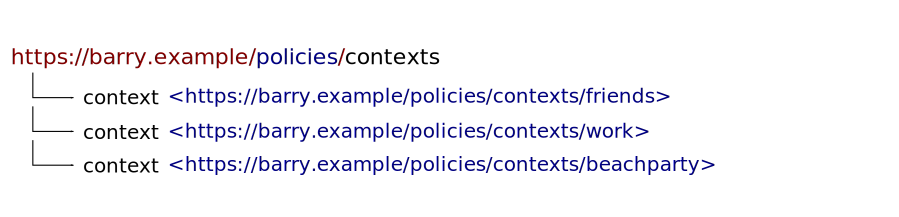
\includegraphics[width=270px]{img/context_tags.pdf}
        \caption{Graph containing all contexts defined by Barry.}
        \label{fig:context_tags}
  \end{center}
\end{figure}

Each context is defined as a resource graph with its own unique URI. To give a context a clear meaning, each defined context has a name and an optional description field (Figure~\ref{fig:context_context}). Since the context's primary function is to define the relationship between a user and a resource, one context can be bound to several resources and users (Figure~\ref{fig:context_context}). For instance, a context graph may contain profile data (e.g. phone numbers, full name, homepages, etc.), wall posts, or even conversations between users (in the form of SIOC\footnote{http://rdfs.org/sioc/spec/} resources).\\

However, since there is no such concept as "pointers" (like the ones found in C/C++), this operation implies that each time a context is assigned to a resource, the resource URI (or literal value) will be copied into the context graph. Another significant drawback resulting from the lack of pointers is that updating a resource in the user's profile must be reflected in all context graphs containing that particular resource.\\

\begin{figure}[h]
  \begin{center}
    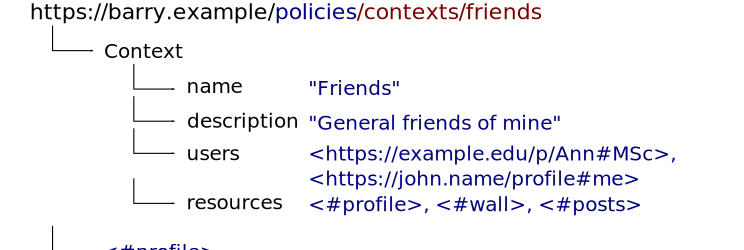
\includegraphics[width=240px]{img/context_context.pdf}
        \caption{Example of a graph for the context \textit{\#friends}}
        \label{fig:context_context}
  \end{center}
\end{figure}

For example, let's consider that Barry assigns the \verb+#friends+ context to his phone number, thus limiting access to this resource. In case this particular context does not exist, the system creates a new context graph, with the URI \textit{https://barry.example/policies/contexts/friends} (Figure~\ref{fig:context_context}). Since the phone number is part of the user profile, the system creates a pointed graph called \textit{<\#profile>} in which it copies the phone number entry. Next, Barry wants to allow Ann to view his phone number. To do this, he has to assign the same context label (i.e. \verb+#friends+) to the user Ann, which is identified by her WebID. The system will now add Ann's WebID to the list of users to which the context \verb+#friends+ has been assigned to (Figure~\ref{fig:context_context}).\\

Several contexts can be assigned to a resource or to a user. Users in the same proximity level can have different contexts, corresponding to different resources, and each user can only see the resources assigned to them. It should be noted that if the user has no defined access control policies, then all the resources they own are publicly available by default.\\

Let us now take a look at the algorithm that is applied in order to match users and resources to contexts, each time a request is received by the system.


\subsubsection{Context matching algorithm}
\label{subsec:context_algo}
Figure~\ref{fig:context_matching} presents a simple algorithm, describing the process of context matching. The goal of this process is to finally return a \textit{unique view} of requested resources (e.g. a user's profile, a wall, a conversation, etc.), based on their corresponding level of access.\\

\begin{figure}[h]
  \begin{center}
    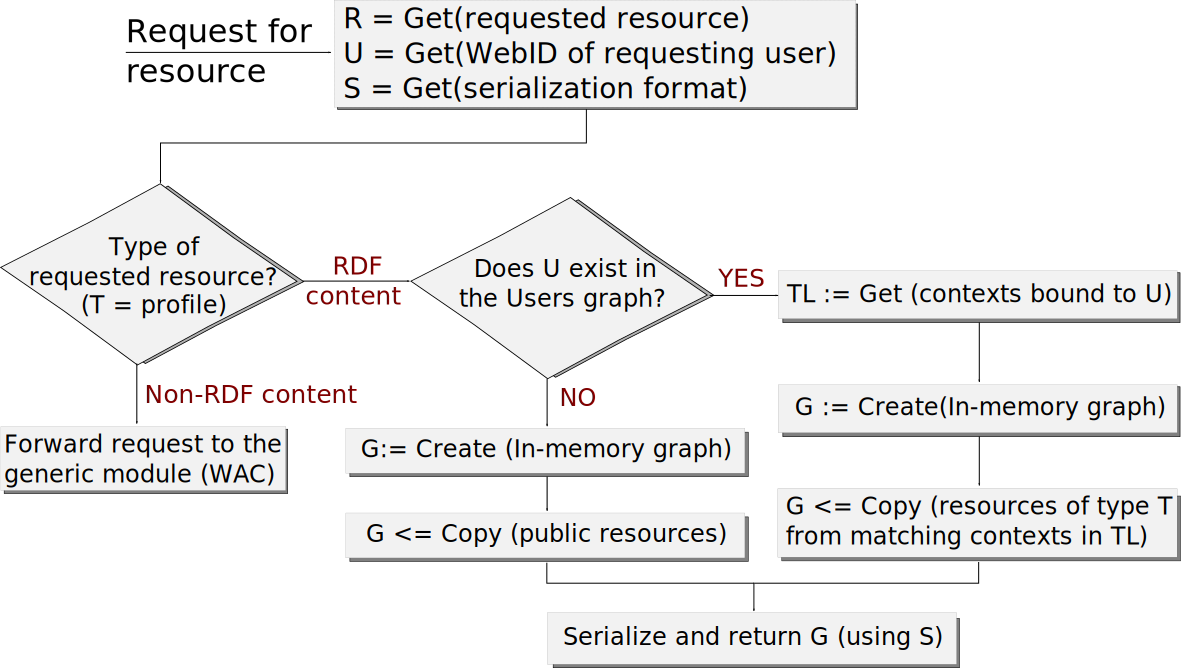
\includegraphics[width=270px]{img/algorithm-matching.pdf}
        \caption{Context matching algorithm.}
        \label{fig:context_matching}
  \end{center}
\end{figure}

The information contained in the \textit{Request} includes the type of the requested resource (T), the WebID of the requester (U) and the data serialization format (S) for the response (e.g. Turtle, RDF/XML, N3, etc.). At this point, we assume that the requesting user has already been authenticated at the moment of the request. If the user has not been authenticated, only the public view of the requested resource is returned.\\

The following step of the algorithm is to lookup the requester in the graph of users belonging to the resource owner. If there is no match, the requester receives only the public view of the requested resource. Otherwise, all contexts assigned to the requester's WebID are extracted, and a list of all contexts URIs (TL) is created.\\

The next step is to create a temporary, in-memory graph (G), to store only the resources matching the requester's access policies. This graph will only be used during the processing of the algorithm, to hold the contents of the reply.\\

Once the graph has been created, it is time to copy all resources belonging to the list of contexts (TL), and which correspond to the type of the request (e.g. a profile, a wall, a conversation, etc.).\\

Finally, the graph (G) is serialized in the requested format (S) before being returned to the requesting user (U). As soon as the contents of (G) have been sent through HTTP(S), the graph is destroyed and memory is freed.


\subsection{The Relationship Monitor engine}
\label{subsec:rme}
The \textit{Relationship Monitor} engine (RM) is tasked to analyse the dynamicity of relationships between two given users, in order to either provide notifications for potential privacy issues that may arise when disclosing information, or it may even modify existing access control policies for incoming requests (if so configured).\\

The RM applies to two distinct types of actions. First, for assigning context labels when disclosing information, and second for handling a request for a resource.

\subsubsection{Assigning context labels}
When a user intends to limit the audience for some of his/her private information (e.g. religious views, sexual orientation, etc.), he/she can assign one or more context labels to the information that is to be protected, as well as to the audience in order to indicate who can access the information.\\
	
During this labelling process, the RM analyses user interaction data from the Relationship History database (Figure~\ref{fig:acs_architecture}), corresponding to the selected audience. Typical examples of user interactions include sharing a picture within a specific context (i.e. \verb+#closefriends+), explicitly changing a user's proximity level, excluding a user from a given context (without permanently removing him/her) when sharing a resource, the number of times users exchange messages (as a function of time), etc.\\

We can imagine that during a user's online activity, several interactions are considered pertinent by the RM. The user should always be allowed to select which types of interactions he/she considers pertinent, or potentially be allowed to create new interaction types. However, since we have not yet implemented the RM in a real application, we will restrict ourselves to proposing several types as follows:

\begin{enumerate}
\item Explicitly sharing a resource (i.e. photo, video, file) with a user.
\item Explicitly sharing profile information (i.e. phone number, email address, etc.) with a user.
\item Assigning a context label to a user, and implicitly a proximity level, since contexts are bound to one or more proximity levels.
\item Removing a context label from a user.
\item Assigning a proximity level to a user.
\item Modifying the proximity level for a user, either manually or by assigning/removing context labels.
\end{enumerate}

Based on the interactions in Relationship History database, the RM may alert the user (i.e. provide visual indications) to a possible change in their relationship. For instance, a warning message may appear if the resource owner is in the process of assigning a context label (which corresponds to a specific proximity level) to a user which is in a more distant proximity level.

\subsubsection{Handling requests}
When requests are received, they are first processed by the RM in order to be classified into two major categories, based on the relationship between the requesting user and the owner of the requested resource (Figure~\ref{fig:algorithm_rme}).\\

In the first category, no predefined privacy policy exists for the requesting user, and the requesting user is not related to the resource owner or any of the resource owner's known people. This is typically the case of an unknown user or a user that is not authenticated. At this point, the RM forwards the request directly to the SAC, where predefined privacy policies are applied for the resource in question.\\

In the second category, the requesting user already has a relationship with the resource owner or with one of his/her known people, based on the authentication credentials it provides alongside the request. In this case, two additional sub-categories exist, and the request is handled by the RM according to the type of the proximity distance and contexts between the requesting user and the resource owner.\\

The first sub-category applies to the cases where a less dynamic relationship exists between the requesting user and the owner of the resource. Please note that through configuration options which are out of scope for the algorithm presented in Figure~\ref{fig:algorithm_rme}, resource owners have the possibility to deliberately disable the RM for relationships they consider less likely to be susceptible to dynamic changes. For example, people labelled as \verb+#family+ or \verb+#girlfriend+. By default, the RM is disabled for users belonging to the \textit{intimate} proximity level.\\

The second sub-category applies to all requesting users that have a dynamic relationship with the resource owner. A history of all interactions between the requesting user and the resource owner is kept in the \textit{Relationship History} database (Fig.~\ref{fig:acs_architecture}).\\

The RM decides whether or not to allow access to resources, based on existing privacy policies defined by the SAC engine, as well as based on data from the Relationship History database corresponding to the relationship between the requesting user and the resource owner. If so configured, the RM can potentially add, update or remove existing rules within the SAC or theoretically, on local and/or remote access control systems like the ones presented in Section~\ref{subsec:sem_acl}. The RM may also support an \textit{unsupervised operation mode}, though this is considered as future work. The unsupervised operation mode would normally involve taking access control decisions based on decision factors resulted from machine learning or the user's decision history, without awaiting user input. However, unless properly configured, the unsupervised operation mode may provide unwanted results and should be activated upon explicit request from the user. Additionally, the RM may be disabled at any time, leaving the SAC in charge of handling all access control.\\

Currently, two metrics are utilized during RM's decision making process. They are the \textit{proximity distance} and the \textit{contexts}. Next, we will go through a typical decision making process for our protagonists, Ann and Barry.

\subsubsection{RM's decision making process}
Before beginning, we would like to mention that the user's social interactions can only be monitored if the RM is part of the social Web application.\\

The algorithm behind the RM's decision making process can be seen in Figure~\ref{fig:algorithm_rme}.\\

\begin{figure}[h]
  \begin{center}
    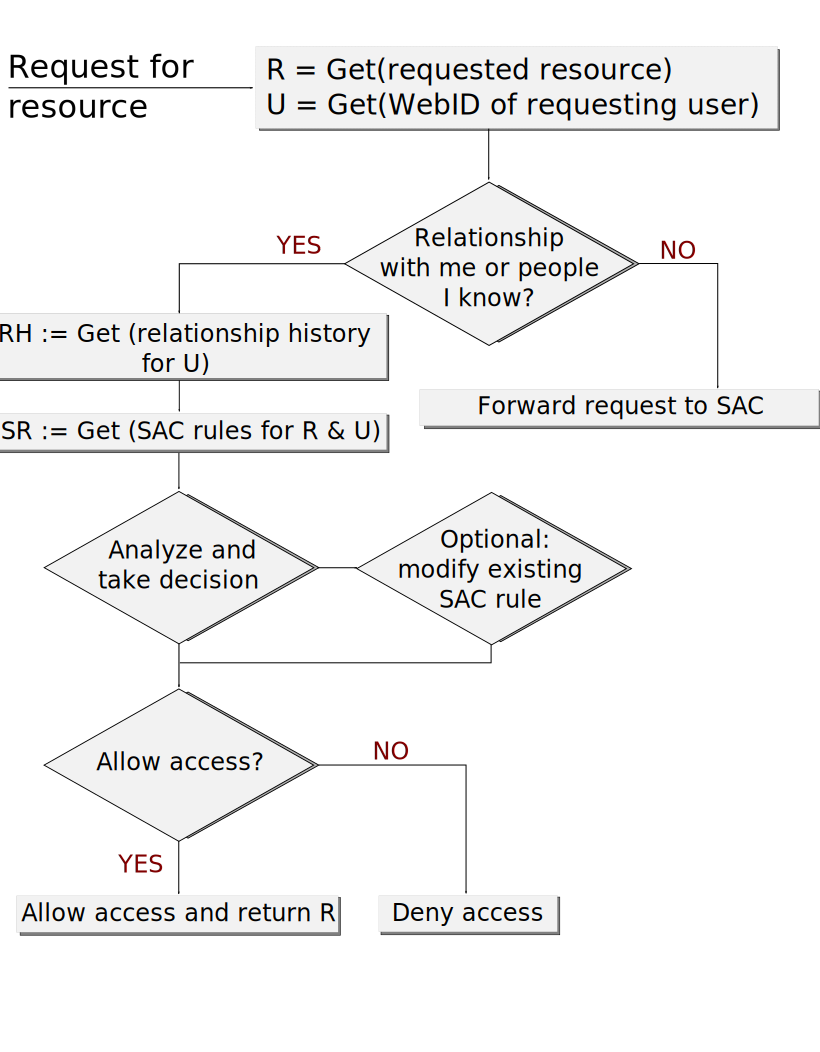
\includegraphics[width=270px]{img/algorithm-rme.pdf}
        \caption{RM's decision making process.}
        \label{fig:algorithm_rme}
  \end{center}
\end{figure}

The information contained in the \textit{Request} includes the requested resource (R) and the WebID of the requester (U). At this point, we also assume that the requesting user has already been authenticated at the moment of the request. If the user has not been authenticated, the process will consider the user to be \textit{undetermined} (i.e. anyone with public access).\\

The following step is to decide if the user in question has any relationships with the resource owner or people known by the resource owner. This step is achieved by querying the Relationship History database to find occurrences of interactions between the requester and the resource owner, or by searching if the requesting user is a friend of the resource owner or if he/she is known by one of the owner's friends (i.e. friend of a friend).\\

If the two users have previously interacted with each other, a graph (RH) containing the list of interactions will be created. Additionally, all static access control rules corresponding to the user (U) and resource (R) will be imported from the policies database and stored in a new graph (SR).\\

Based on the the contents of (RH) and (SR), the system will analyse and decide how to proceed next. If the data from (RH) is found to be heavily conflicting with the rules in (SR) and if the RM engine is operating in \textit{unsupervised mode}, the system may optionally modify existing SAC rules. For example, if the requester was deemed to have changed proximity distance either through an evolution of his/her relationship towards the resource owner, or because the resource owner explicitly modified the user's proximity distance, the system may be able to reflect this change in the SAC rules.\\

Once the final decision is made, the RM engine will either grant access or deny access to the requested resource.


\subsection{Relationship History database}
The Relationship History database stores information based on the user's interactions. The interactions are expressed as triples using the  Activity Base Schema~\cite{activityschema2012}, a base set of object types and verbs for use with Activity Streams.\\

Figure~\ref{fig:relation_history} illustrates a typical case of saved interaction, triggered by the action that Barry has "made friends" with Ann. In this case, the actor is Barry, since it was him who initiated the action. We can imagine a similar situation but with the roles reversed, if Ann performed an action with respect to Barry.\\

\begin{figure}[h]
  \begin{center}
    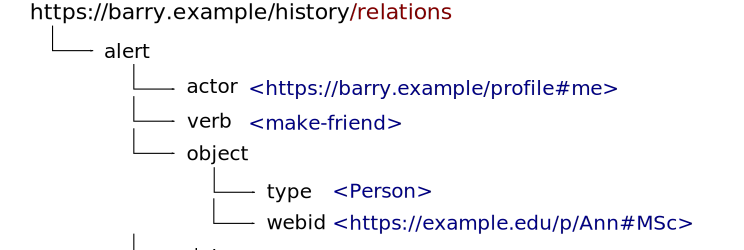
\includegraphics[width=270px]{img/relation_history.pdf}
        \caption{Example of an interaction between Barry and Ann.}
        \label{fig:relation_history}
  \end{center}
\end{figure}

It should be noted that if a user should feel at any time that collecting this information may potentially result in too much exposure of his/her private data, he/she should have the option to disable the Relationship History.

\section{Conclusion}
We believe that based on different contexts and situations, access to resources can be handled differently, especially when coupled with dynamic user relationships. In this chapter we have introduced our third contribution, a social access control service for Web applications, comprised of two distinct sub-services: a \textit{Static Access Control} (SAC) engine and a \textit{Relationship Monitor} engine (RM). Due to existing access control alternatives which handle access control for static documents (Section~\ref{subsec:sem_acl}), our solution is focused on protecting the privacy of Linked Data resources generated by users (e.g. profile data, wall posts, conversations, etc.).\\

The \textit{Static Access Control} engine handles access to user-generated resources, based on predefined privacy policies. The process of permitting/denying access to a resource is quite straightforward, and it involves matching the user performing the request to a list of resources matching the same \textit{context} label. The goal of this process is to finally return a \textit{unique view} of requested resources (e.g. a user's profile), matching to the level of access corresponding to the requesting user.\\

The \textit{Relationship Monitor} engine (RM) relies on metrics such as \textit{context} and \textit{proximity distance} together with a relationship history between the involved actors, in order to either provide notifications for potential privacy issues that may arise when disclosing information, or even to modify existing access control policies for incoming requests (if so configured). The RM applies to two distinct types of actions. First, it is used when assigning context labels when disclosing information, and second for handling a request for a resource.\\

The static access control engine was implemented as a module for MyProfile (Chapter~\ref{ch:implementations}). Unfortunately, we were not able to implement the RM engine for a real application, and therefore we consider this as future work.


% Implementations
\chapter{Building a decentralized social semantic Web}
\label{ch:implementations}
The Semantic Web is envisioned as a decentralised world-wide information space for sharing machine-readable data with a minimum of integration costs. Its two core challenges are the distributed modelling of the world with a shared data model, and the infrastructure where data and schemas can be published, found and used. Users benefit from getting information "raw and now" and in portable data formats, usually based on RDF, which can then be published on the Web. Others can read the data and publish their own information, linking to existing resources. This forms a distributed model of the world. It allows the user to pick any application to view and work with the same data, for example to see Ann's published address in your address book.\\

At the same time, documents on the Web have always been addressed with URIs (often referred to as Uniform Resource Locators, URLs). This is useful because it means that we can easily make RDF statements about Web pages, but it is also dangerous because we can easily mix up Web pages and the \textit{things}, or \textit{resources}, that are described on the page (cf. Section~\ref{subsec:webid_uri}).\\

A truly decentralized social Web application, based on Semantic Web technologies, requires several key components. It must be able to offer decentralized user identity, secure authentication, semantic data storage, to apply Create-Read-Update-Delete (CRUD) operations to resources, to offer increased privacy through access control, and most importantly, to be interoperable with other applications in terms of data exchange (e.g. content sharing, messaging, activity notifications, etc.).\\

This chapter intends to be a guide on how to proceed with building a decentralized social Web application. It also reflects our implementation efforts in the form of MyProfile, a decentralized identity platform, which serves as a demo for the theoretical solutions we have proposed in the previous chapters. We will explain our conceptual decisions as well as any technical limitations we ran into during the development of MyProfile.\\

\section{MyProfile}
The project \textit{MyProfile}~\cite{sambra2011myprofile} is a reflection of all efforts we have made over the course of this thesis. It intends to provide to users the privacy they deserve for the data they produce and own. It offers a unified user account, which centralizes the user's data and puts it under the user's control, and also on a device the user controls. It is a radical change from the \textit{walled gardens} of today's Web, where data are trapped in \textit{silos}.\\

The project was launched in April 2011, and it was funded entirely by TELECOM SudParis, member of group Institut Mines-TELECOM. It offers a unique identity platform, which takes advantage of Semantic Web technologies, so that users no longer need to invest time and effort into building complex profiles on the numerous websites/services they currently use. The profile is stored on a Web accessible device where only the user has access -- the user's computer, a dedicated server, or ideally a plug computer like the FreedomBox\footnote{http://www.freedomboxfoundation.org/}. This way, the user controls both the physical data and who can access it.

MyProfile also offers services that do not require a local profile. Any user is able to \textit{view} his/her profile data in a friendlier and attractive way. While viewing the profile data, the platform displays the user's list of known people (i.e. friends), some basic information for each friend (e.g. full name, nickname, email, blog), as well as a text mention in case the relationship is bidirectional (i.e. "Has you as friend.").\\

Once authenticated, additional functionalities become available. For example, users can post messages to a public \textit{wall}, which is a common place for all users to write about news, events, social updates, etc. Users can also \textit{subscribe} to local services in order to have their own private wall, which is only available to their list of known people. Subscribing also allows users to send and receive private messages, as well as notifications when other users have posted something on their private wall.\\

The source code for MyProfile has been released under an MIT license (less restrictive compared to other open source licenses), and it is publicly available on GitHub under MyProfile\footnote{https://github.com/MyProfile/myprofile}. For portability and deployment reasons, the platform was mainly written in PHP and JavaScript. It relies on Virtuoso\footnote{http://virtuoso.openlinksw.com/} to facilitate RDF-triple storage and SPARQL queries for cached profiles. A running demo of MyProfile can be accessed at https://my-profile.eu/.\\

Let us now take a detailed look at each platform component, starting with the user profiles.

\subsection{Creating a user profile}
MyProfile uses WebID as the main mechanism for user profiles, allowing for an increased interoperability. Depending on the user's social interactions on the Web, the profile could also extended to contain resources like blog and forum posts, or even mailing list messages, all described using dedicated ontologies. We can safely say that the user's profile can contain an unlimited number of resources, as long as they can be expressed using standard Semantic Web vocabularies.\\

The WebID URIs follow common Representational State Transfer (REST) structures. Each user is assigned a unique URI, composed of three main parts:
\begin{enumerate}
\item The server's IP address or fully qualified domain name (FQDN), i.e. \verb+https://my-profile.eu/+
\item The directory structure under which the profile is located, i.e \verb+people/barry/+ 
\item The profile document with a fragment identifier denoting the user, i.e. \verb+card#me+
\end{enumerate}

Finally, the complete WebID URI becomes the following:\\ 

\verb+https://my-profile.eu/people/barry/card#me+\\

The minimum information required for a new profile is comprised of the \textit{local username} (i.e. barry) and the user's full name, may it be real or not. Optionally, the user can provide an email address that will only be used for account recovery purposes, and is never disclosed to anyone else.

\subsubsection{Issuing client certificates}
During the account creation process, a client certificate will be issued and automatically installed in the browser, as well as have its public key added to the user profile. The system relies on HTML5 \textit{<keygen>} element, to guarantee that the private key is never disclosed, not even to the server. The \textit{keygen} element exists to facilitate generation of key material, and submission of the public key in the Signed Public Key and Challenge (SPKAC) \cite{ellison1999spki} format. The process is similar to generating Certification Signing Requests (CSRs), where an encoded public key can then be manipulated using OpenSSL\footnote{http://www.openssl.org/}.\\

The process of issuing the X.509~\cite{solo1999internet} client certificate has proven to be quite challenging. The main reason is due to how PKI works when it comes to signing CSRs, more specifically the dependence on a Certification Authority (CA). Basically, once the public key and the user's full name have been sent by the browser, the server must transform them into a valid CSR and sign them with the CA's key. The problem we ran into, while using PHP, was that there is no support for this kind of cryptographic operations. Therefore, we ended up using OpenSSL through a system call.\\

Another issue related to X.509 certificates concerns the way they are sent back to the client. Once the user submits the form containing the HTML5 \textit{keygen} element, the server must return the certificate by responding with the proper content type, set to \textit{application/x-x509-user-cert}. The problem lies in the fact that by setting a specific content type for sending the certificate, no other data can be sent along the certificate, meaning that the server cannot send a page to indicate the success of the operation. Unaware users may believe that no action was performed and they might click the submit button again.

\subsubsection{Publishing the profile}
MyProfile user profiles are expressed as Turtle~\cite{beckett2008turtle} documents by default, in order to align with the WebID specification. However, users have the option to export their profiles using different serialization formats, like RDF/XML~\cite{beckett2004rdf}, N3~\cite{berners2000primer} or JSON~\cite{crockford2006application}.\\

When a request for the profile document arrives, the Web server must decide which content type to serve. Currently, MyProfile uses \textit{.htaccess} files to intercept requests and perform content negotiation based on two content types, \textit{text/turtle} and \textit{text/html}.\\

\begin{example}[h]
\begin{minted}{apache}
Options -MultiViews -Indexes
AddType "text/turtle" .ttl
RewriteEngine On
RewriteBase /people/barry/
RewriteCond %{HTTP_ACCEPT} !text/turtle
RewriteRule ^card$ https://my-profile.eu/view?webid=<WebID> [R=303]
RewriteCond %{HTTP_ACCEPT} text/turtle
RewriteRule ^card$ card.ttl [L]
\end{minted}
\caption{Contents of a .htaccess file for user profiles.}
\label{ex:htaccess}
\end{example}

Example~\ref{ex:htaccess} displays the contents of a .htaccess file, for user \textit{barry}. Here we have two conditions, expressed using the \textit{RewriteCond} directive. The first condition states that if the Accept header of the request is different from \textit{text/turtle}, then it will serve HTML by triggering the \textit{RewriteRule} that redirects the user to the special view page. On the other hand, if the Accept header is explicitly set to \textit{text/turtle}, it will serve the RDF document instead (i.e. card.ttl).

\subsection{Viewing profiles}
MyProfile provides a visually appealing rendering of WebID profiles, regardless if the user is local or not (Figure~\ref{fig:view_html}). To read and process RDF data, we have decided to use EasyRdf, a PHP library designed to make it easy to consume and produce RDF as graph of PHP objects that can then be walked around to get the data to be placed on the page.\\

\begin{figure}[h]
  \begin{center}
    \includegraphics[width=350px]{img/screens/view_html.jpg}
        \caption{Rendering of a profile.}
        \label{fig:view_html}
  \end{center}
\end{figure}

The view page provides additional information for the user's known people, in the form of full name, nickname, email, phone number and blog. If the user is authenticated and viewing his/her own profile, a text mention "Has you as friend." will appear next to the known person if that person also has a \textit{foaf:knows} relation pointing back (Figure~\ref{fig:view_html}). Additionally, the view page offers a series of buttons that allow to quickly remove known people from the user's profile, to view their wall and even to explore their social graph, as seen in Figure~\ref{fig:view_html}.\\

The same page allows users to lookup other people by searching for names, nicknames and WebID URIs within the cached public profiles of people that have used the platform at one point or the other. If the user performing the lookup is authenticated and has a local profile, he/she can then simply press a button to add one or more search results to his/her list of known people.

\subsection{Social walls and activity streams}
The \textit{social wall} is a familiar concept in social networks. It allows users to post updates about their life, to talk about their interests, to share links and content, or to openly communicate with other people (Figure~\ref{fig:public_wall}).\\

\begin{figure}[h]
  \begin{center}
    \includegraphics[width=350px]{img/screens/public_wall.jpg}
        \caption{MyProfile public wall.}
        \label{fig:public_wall}
  \end{center}
\end{figure}

MyProfile offers two types of social walls. The first type is a platform-wide, shared public wall. Its purpose is to allow users to quickly post public information, that may also be of use to people outside their friends list. To be able to post on the public wall, users need to be authenticated through WebID-TLS (see Section~\ref{sec:webid-auth}). The second type is a private, restricted access wall, which is only available to the user's known people (i.e. described through \textit{foaf:knows} relations). Other people can express their level of appreciation towards wall posts by either liking or disliking them.\\

The activity stream is a derivative of the social wall. It is a collection of all posts written by people the user knows, and presented in a chronological order. Its purpose is to allow users to keep track of updates from their friends, without having to visit the private walls of their friends.\\

Based on the content type of the \textit{Accept}, clients can request either an HTML view of the social wall, or more importantly, an RDF view. Currently, only Turtle and RDF/XML serialisation are available for the RDF view. Wall posts are represented using the SIOC~\cite{breslin2005towards} ontology. Example~\ref{ex:wall_paging} displays how pagination is supported through URI requests, though it does not reflect in the RDF data.

\begin{example}[h]
\begin{minted}{c}
GET /wall.php?offset=20 HTTP/1.1
Host: my-profile.eu
Accept: text/turtle
\end{minted}
\caption{RDF social wall pagination.}
\label{ex:wall_paging}
\end{example}

\subsection{Account recovery and pairing}

\subsubsection{Account recovery}
Since MyProfile uses WebID-TLS for authentication, if a user cannot use his/her certificate any longer and regardless of the reason, there must exist the possibility to recover access to his/her account. Account recovery will work only if the user has already provided an email address for this purpose, either at the moment of creating the WebID, or through the preferences page.\\

The first step of the procedure to recover access to a MyProfile account involves providing the user's WebID. Once this information is submitted, the system will generate a one-time password (OTP)~\cite{haller1995s} in the form of a hash (i.e. a string of alphanumeric characters) and bind it to the WebID submitted by the user. Finally, an email is sent to the address initially specified by the user when he/she created the account. The email contains a pre-formatted link containing the OTP, which enables the user to authenticate as if he/she was authenticating through WebID-TLS. Once authenticated, the user has the possibility to issue new certificates, which will be automatically added to his/her WebID profile. If the authentication was successful, the OTP is removed so it can never be used again to gain access to this particular account.

\subsubsection{Pairing}
The pairing process was created to address the difficulty of having to manage client certificates across different browsers and devices. Until now, users had to manually export certificates from one browser and then import them into a different browser or device. The pairing process is different from account recovery, though it can be used to provide a similar end result.\\

In this case, users must first authenticate (either through WebID-TLS or by using the account recovery feature) in order to access their preferences page. This page allows them to generate a 6 digit one-time numeric password, which we call \textit{PIN} (Figure~\ref{fig:pairing_pin}). To avoid brute-force attacks on the PIN, we have decide to limit its validity period to one minute, starting from the moment it was issued. A new PIN must be generated if the user is not able to type it within the given time frame on the other device.\\

\begin{figure}[htbp]
  \begin{center}
    \includegraphics[width=350px]{img/screens/pin_gen.jpg}
        \caption{Generating a pairing PIN.}
        \label{fig:pairing_pin}
  \end{center}
\end{figure}

\subsection{Statistics}
MyProfile is currently the de facto service provider when it comes to issuing WebIDs, hosting close to 500 WebIDs, and being visited daily by more than 30 different users. It is also the main reference when it comes to implementing a decentralized social Web application.\\

MyProfile has been the subject in different workshops and conferences around the world, as well as in different talks and presentations in the past two years:

\begin{itemize}
\item 2013: Mentioned in "Let's tear down these walls" talk at SIGINT13\footnote{https://sigint.ccc.de/} in Cologne (Germany), an annual hacker conference covering both technical and social aspects of our digital society.

\item 2013: Mentioned at OuiShare Fest\footnote{http://ouisharefest.com/} in Paris, a conference about the collaborative economy in Europe.

\item 2012: Included by the Free Software Foundation Europe\footnote{http://fsfe.org/} in their list of different approaches for Cloud Computing. The development of MyProfile is also followed by the FreedomBox Foundation\footnote{http://www.freedomboxfoundation.org/}.

\item 2011: Presented by me in a panel called "Alternatives to Facebook" during the Social Media Week Berlin\footnote{http://socialmediaweek.org/berlin/} event.

\item 2011: Mentioned in Heise\footnote{http://www.heise.de/}, a respectable German online news magazine.
\end{itemize}


\section{WebID authentication}
WebID-TLS authentication plays a crucial role in MyProfile. On one hand it allows any authenticated user to post messages on walls or contact other people, regardless if they have a local account or not. On the other hand, local users that have been authenticated can also easily update their profiles, issue new certificates or manage their friends.\\

There exists two different WebID-TLS authentication approaches, either perform the WebID-TLS verification locally, or use a third party WebID-TLS authentication service. We have developed two libraries, written in PHP, which cover both approaches. The libraries have been released under the MIT license, and are publicly available on GitHub under WebIDauth\footnote{https://github.com/organizations/WebIDauth}. In the following subsections we will describe both libraries, as well as how the Web server must be configured to offer WebID-TLS authentication. 

\subsection{Configuring the Web server}
WebID-TLS authentication requires the Web server to be configured in a special way. For portability and deployment reasons, we have decided to use the Apache~2 Web server\footnote{https://httpd.apache.org/}.\\

To request client certificates from users, the Web server configuration file must include the following directives:
\begin{itemize}
\item \verb+SSLVerifyClient optional_no_ca+ -- skip verifying the CA, since WebID does not operate based on standard PKI trust
\item \verb+SSLVerifyDepth 1+ -- stop after the initial certificate, to avoid recursively traversing the trust chain
\item \verb!SSLOptions +ExportCertData! -- export certificate contents to the environment, so that it can be used by other programs (e.g. PHP, Python, Java, etc.)
\end{itemize}

The above directives must be part of the \textit{VirtualHost} configuration, as it is no longer possible to place them in \textit{.htaccess} files due to security issues. A full example of the Apache configuration file is provided in the Appendix, under Example~\ref{app:auth_conf}.\\

Please note that in order to allow old browser versions that do not support SSL renegotiation, the following configuration directive must be present:\\

\verb+SSLInsecureRenegotiation on+

However, if this directive is enabled, SSL connections will be vulnerable to the Man-in-the-Middle prefix attack\footnote{http://cve.mitre.org/cgi-bin/cvename.cgi?name=CAN-2009-3555}.

\subsection{WebIDauth}
Local authentication can be achieved by relying on \textit{WebIDauth}, a PHP library implementing WebID-TLS. Its particularity resides in the fact that it allows users to request a \textit{verbose} authentication process, which is useful when debugging a faulty certificate or a user profile.\\

WebIDauth can operate in two modes. In the first mode, its task is to perform WebID-TLS authentication and simply return either \textit{true} or \textit{false}, depending whether the user was successfully authenticated or not. This mode is intended to be used as an authentication method for a local application, usually coupled with a user session. However, operating in this mode also implies configuring the Web server to run over HTTPS, adding to the expenses of hosting the local application by having to buy a server certificate.\\

In the second operation mode, WebIDauth can be used as a Relying Party, a third-party service that provides a WebID-TLS authentication endpoint for Web applications that cannot perform the authentication process themselves. There are several advantages to using a Relying Party service. For instance, it drastically reduces the complexity of having to set up the Web server to allow WebID-TLS authentication. Additionally, the service provider (local application) may not require HTTPS, therefore the owners do not need to pay for a server certificate. We will present in detail how this process is accomplished in the next subsection that deals with delegated authentication.\\

Currently, WebIDauth supports the following functionalities:
\begin{itemize}
\item It initiates the WebID-TLS protocol, by requesting a client certificate from connecting users
\item It checks if the SubjectAltName field contains something else other than the WebID URI, and only processes HTTP URIs
\item It checks if the WebID profile document contains any public keys of type \textit{RSApublickey} and cycles through them looking for a possible match
\item It checks the HTTP request for a variable called \textit{verbose} and if it is set, it displays the contents of the certificate used to connect to the IdP, as well as each step of the WebID-TLS protocol
\end{itemize}

WebIDauth is actively being used for over two years to offer a WebID-TLS authentication service, located at https://auth.my-profile.eu/. Several people have contributed to the source code of this library, improving it in multiple ways. Lately, the service offered by https://auth.my-profile.eu/ handles an average of 2000 authentication requests per month, while in the past year alone it has been accessed by more than 4500 users around the world.

\subsection{WebIDDelegatedAuth}
Delegated WebID-TLS authentication is the process of relying on a third-party service to perform the authentication, and then redirect the user back to the Service Provider, as seen Section~\ref{sec:webid-tls_delegated_auth}. This is currently the default operation mode for MyProfile. The WebIDDelegatedAuth library was created so that Service Providers can offer WebID-TLS authentication in case they are not capable of offering local authentication, or they do not operate over HTTPS. Let us now explore each step of the process.\\

First, the user clicks a login button on the Service Provider (i.e. https://my-profile.eu) and is redirected to the Relying Party (i.e. https://auth.my-profile.eu), thus triggering the authentication process. The Service Provider also appends a variable to the redirection URI, containing the Service Provider's URI:\\ 
\textit{https://auth.my-profile.eu/?authreqissuer=https://my-profile.eu}.\\

Next, the Relying Party uses WebIDauth to perform WebID-TLS authentication. If the user has been successfully authenticated, the Relying Party prepares the redirection request, appending additional arguments to the redirection URI, namely the \textit{webid}, \textit{ts}, \textit{referrer} and \textit{sig}.\\

The aforementioned arguments have the following meanings, as we have seen in Section~\ref{sec:webid-tls_delegated_auth}:

\begin{itemize}
\item \verb+webid+ - https://my-profile.eu/people/barry/card\#me.
\item \verb+ts+ - 2013-05-22CEST16\%3A54\%3A04\%2B02\%3A00
\item \verb+referrer+ - https://auth.my-profile.eu
\item \verb+sig+ - hR5cv9gPn.....MxBbSdq7f.
\end{itemize}

Back on the Service Provider, WebIDDelegatedAuth is used to verify the incoming request, by attempting to find the referrer's public key among a local list of trusted Relying Party URIs. Once the signature and the timestamp have been validated, the Service Provider proceeds to login the WebID \textit{https://my-profile.eu/people/barry/card\#me} belonging to the user. To avoid repeating the process, a session is created and a cookie with a validity period of 24 hours is issued to the user.\\

If you would like to find out how to quickly deploy WebIDDelegatedAuth to enable a Service Provider to offer WebID-TLS authentication for its users, please see Example~\ref{app:webiddelegatedauth} of the Appendix.

\section{Static Access Control}
\label{sec:sac_implem}
The SAC library is used to offer a \textit{unique view} of a user's profile, based on the level of access specific for the agent requesting the information. It uses context labels to match users to the resources to which they are granted access. The same label must be assigned to the resource that is part of the user's profile (e.g. email address, phone number, etc.). As you can notice in Figure~\ref{fig:sac_ui}, users that are displayed as \textit{foaf:knows} relations can be considered both as normal resources to be protected (the icon with the eye), as well as users we want to match against the resources (the person shaped icon).\\

\begin{figure}[h]
  \begin{center}
    \includegraphics[width=270px]{img/screens/sac_ui.jpg}
        \caption{Static Access Control icons displayed when viewing a profile.}
        \label{fig:sac_ui}
  \end{center}
\end{figure}

The library depends on Virtuoso to store graphs containing access control policies. The SPARQL language is used to insert data as well as to query the graphs. The source code is part of MyProfile Project, as the library is intended to be a core component of the platform.

\section{Personal data stores using RWW.I/O}
Offering individual data stores is an important aspect of any decentralized social application, as users must be allowed to choose where they want to host their data, as well as to have complete control over the privacy settings that apply to these data. If possible, data stores should be hosted by devices to which the user has physical access. However, for performance reasons, data stores may be located on third party servers, if users are not concerned by privacy issues.\\

Being invited to work with Sir Tim Berners-Lee on access control for the Semantic Web at the Massachusetts Institute of Technology, has allowed me to develop a Linked Data personal data store platform that implements the Web Access Control~\cite{hollenbach2009using} (WAC) ontology. The code is written in PHP, Python and JavaScript, and is publicly available under an MIT license on Github at \textbf{RWW.io}\footnote{https://github.com/deiu/rww.io}.\\

RWW.I/O stands for \textit{Read-Write-Web Input/Output} and it operates under the assumption that users require a personal data store, where different applications can store data about and for the user, and where data are equally available between applications (Figure~\ref{fig:rww}). The advantage is that different applications can reuse the same data, to offer different functionalities. For example, a contact management application can pull data from the user's profile and modify it at the user's request. The modifications are instantly reflected in the user's profile the next time someone accesses the profile.\\

\begin{figure}[h]
  \begin{center}
    \includegraphics[width=350px]{img/screens/rww.jpg}
        \caption{The RWW.I/O service.}
        \label{fig:rww}
  \end{center}
\end{figure}

\subsection{Creating data stores}
To create their personal data store, users must first choose a desired location for their data. Location is determined based on a unique string of characters defined by the user, similar to an account name, which is then transformed into a subdomain. In other words, the account name \textit{deiu} is used to create the subdomain \verb+https://deiu.rww.io/+, which in turn becomes the user's personal data store. Users can have an unlimited number of data stores, regardless of where they are located.\\

Creating the data store implies only setting up the subdomain. To own the data store, users must first authenticate using WebID-TLS and then claim the subdomain by creating an access control rule for the root directory (i.e. the subdomain itself). This step can be done either through the access control UI, or directly by performing an HTTP POST of a Turtle document containing the ACL triples. If users do not have a WebID, they can create a minimal one locally, and then use it to authenticate and claim ownership of the data store.\\

The platform supports full Create-Read-Update-Delete (CRUD) operations, following the REST standards. Documents and directories can be created by performing HTTP requests such as POST, PUT and MKCOL (i.e. new directories), following the requirements we presented at the beginning of the chapter. The \textit{Content-Type} HTTP header plays a central role to interpreting the requests and deciding whether to store data as triples or as binary files. As RWW.I/O is not intended to be a fully-fledged cloud service, only a handful of content types are supported.\\

In order to detect a conflict when overwriting a resource through HTTP PUT, we are using HTTP/1.1 features including entity tags (ETags)~\cite{nielsen1999editing}, the various If-* preconditions header field (e.g. \verb+If-Match+, \verb+If-None-Match+, etc.) and HEAD requests.

\subsection{Managing access control for resources}
Access control rules for the data store resources are specified using the Web Access Control ontology. The data store was designed to use one ACL file for each document, thus separating the metadata containing the access control rules from the document they protect. The naming convention for the metadata files involves using a \verb+.meta+ prefix before the filename. For example, if a given file is named \textit{photo.jpg}, the corresponding metadata file will be named \textit{.meta.photo.jpg}, and it will be situated at the same directory level. Assigning an ACL metadata file for each document offers the advantage of flexible access control management, especially for resources for which control is handled by third party users or even applications (i.e. a data store within a data store).\\

Managing access control rules can be achieved either through an ACL user interface (UI), or by manipulating the metadata files through HTTP verbs (i.e. POST, PUT, DELETE). The UI offers minimal functionalities, as seen in Figure~\ref{fig:acl_ui}. If the \textit{Default} checkbox is enabled and the resource is a directory, the rules will apply by default for all resources in that specific directory. The default rules can be superseded later on by creating metadata files for those resources.\\

\begin{figure}[h]
  \begin{center}
    \includegraphics[width=250px]{img/screens/acl_ui.jpg}
        \caption{ACL user interface.}
        \label{fig:acl_ui}
  \end{center}
\end{figure}

To conform to the best practices of using the Web, the UI also uses HTTP verbs to create and modify metadata files. This way, users are able to create workspaces (i.e. dedicated data stores) for third-party applications, which enable the applications to handle their own ACL management, regardless of who owns the data store. Example~\ref{ex:metafile_profile} describes the process of creating a metafile for a WebID protected document.\\

\begin{example}[h]
\begin{minted}{c}
PUT /private/protected.ttl HTTP/1.1
Host: deiu.rww.io
Content-Type: text/turtle
Content-Length:407

Payload:
\end{minted}
\begin{minted}{turtle}
@prefix rdf: <http://www.w3.org/1999/02/22-rdf-syntax-ns#> .
@prefix WAC: <http://www.w3.org/ns/auth/acl#> .
@prefix foaf: <http://xmlns.com/foaf/0.1/#> .
<>
    WAC:accessTo <> ;
    WAC:agent <https://my-profile.eu/people/deiu/card#me> ;
    WAC:mode <WAC:Read>, <WAC:Write> .

<#protected.ttl>
    WAC:accessTo <protected.ttl> ;
    WAC:agent <https://my-profile.eu/people/deiu/card#me> ;
    WAC:mode <WAC:Read>, <WAC:Write> .
\end{minted}
\caption{Creating a metafile for the document \textit{/private/protected.ttl}.}
\label{ex:metafile_profile}
\end{example}

Creating a metafile for \verb+/private/protected.ttl+ implies creating two access control rules. The first rule, <>, applies to the document itself (i.e. https://deiu.rww.io/private/.meta.protected.ttl), and it states that only the agent identified by the WebID \textit{https://my-profile.eu/people/deiu/card\#me} is allowed to perform \textit{Read} and \textit{Write} operations on the document in question. The second rule is for the document the metafile protects (i.e. \verb+/private/protected.ttl+). The rule states that the Read and Write operations are allowed for the agent identified by the WebID URI.

\subsection{Application workspaces - a complete example}
This section will provide a complete example, explaining how users can create dedicated workspaces for third-party applications, in this case a photo viewing application. We assume that Barry uses RWW.I/O as a personal data store, located at \textit{https://barry.rww.io/}.\\

\subsubsection{Step 1}
At some point, Barry decides that he wants to use a photo viewing service, namely "myPhotos". To begin using this service, Barry must first login into https://myphotos.com with his WebID. Once authenticated, myPhotos creates a unique resource, containing a list of required data store permissions corresponding to several functionalities it can offer, which then binds to Barry's WebID. The permissions resource is available for Barry to inspect at http://myphotos.com/permissions/<sha1> (Example~\ref{ex:myphotos_permissions}).\\

\begin{example}[h]
\begin{minted}{turtle}
@prefix wapp: <http://ns.rww.io/wapp#> .
<>
    wapp:redirects <https://myphotos.com> ;
    wapp:permission <#a> ;
    wapp:permission <#b> ;
    wapp:permission <#c> ;
    wapp:permission <#d> .
<#a>
    wapp:kind wapp:mandatory ;
    wapp:requires wapp:workspace ;
    wapp:requires wapp:read ;
    wapp:requires wapp:write ;
    wapp:usage <http://dbpedia.org/Photo> ;
    wapp:suggestedName "photos" .
<#b>
    wapp:kind wapp:mandatory ;
    wapp:requires wapp:workspace ;
    wapp:requires wapp:exclusive ;
    wapp:suggestedName "myphotos" ;
    wapp:description "Photo viewing application." .
<#c>
    wapp:kind ws:optional ;
    wapp:advertiseInProfile [
        wapp:comment "myPhoto is cool!"
    ] .
<#d>
    wapp:kind ws:functional ;
    wapp:requires wapp:workspace ;
    wapp:requires wapp:read ;
    wapp:requires wapp:write ;
    wapp:usage <http://dbpedia.org/Tag> ;
    wapp:suggestedName "tags" .
\end{minted}
\caption{List of permissions required by the application \textit{myPhoto}.}
\label{ex:myphotos_permissions}
\end{example}

\subsubsection{Step 2}
After the registration process (and perhaps payment), myPhotos redirects the user to his/her personal data store service, while also passing the permission resource as an HTTP request parameter: https://barry.rww.io/permissions?permissions=<url encoding of http://myphotos.com/permissions/<sha1> >.\\

Barry's data store service fetches the permission resource from myPhotos, and then generates a form so that each permission can be accepted or rejected by the user. If all \textit{mandatory} permissions are accepted, the data store service can process and update the permissions resource with the user approvals and rejections. Since in this case Barry has decided that he does not want to add the third permission (i.e. <\#c> -- which would add and advertisement comment to his profile), so it will be removed from the list of permissions.\\

Additionally, based on the \textit{wapp:usage} specified in the permissions list, the data store service will assign specific workspace URIs for each accepted permission (Example~\ref{ex:barry_updated_permissions}). Once the permissions list has been updated, the data store service will POST the updated permissions list containing the triples in Example~\ref{ex:barry_updated_permissions}, to myPhoto:

\begin{example}[h]
\begin{minted}{console}
Command:

curl -X POST \textbackslash
     -H "Content-Type: text/turtle" \textbackslash
     -E rww.io-cert.pem \textbackslash
     -d @updated-permissions.ttl \textbackslash
     https://myphotos.com/permissions/<sha1> 

Contents of updated-permissions.ttl:
\end{minted}
\begin{minted}{turtle}
@prefix wapp: <http://ns.rww.io/wapp#> .
<#a> wapp:status ws:Accepted ;
    wapp:workspace <https://barry.rww.io/photos/> .

<#b> ws:status ws:Accepted ;
    wapp:workspace <https://barry.rww.io/apps/myphotos/> .

<#c> ws:status ws:Rejected .

<#d> ws:status ws:Accepted ;
    wapp:workspace <https://barry.rww.io/tags/> .
\end{minted}
\caption{Returning the list of updated permissions.}
\label{ex:barry_updated_permissions}
\end{example}

\subsubsection{Step 3}
After having accepted the permissions, a trust relation must be created between myPhoto's Web agent (i.e. http://myphotos.com/profile\#agent) and Barry. The trust relationship is very important, as it allows the application to act on his behalf (Section~\ref{sec:webid-delegated-access}) while manipulating resources on Barry's data store.\\

\begin{example}[h]
\begin{minted}{turtle}
@prefix rdf: <http://www.w3.org/1999/02/22-rdf-syntax-ns#> .
@prefix foaf: <http://xmlns.com/foaf/0.1/> .
@prefix wapp: <http://ns.rww.io/wapp#> .

<>
    a foaf:PersonalProfileDocument ;
    foaf:primaryTopic <#me> .

<#me>
    a foaf:Person ;
    foaf:name "Barry" ;
    wapp:uses <#myphotos> .

<#myphotos> 
    a wapp:app ;
    wapp:service <https://myphotos.com/> ;
    wapp:endpoint <https://barry.rww.io/apps/myphotos/> ;
    wapp:description "Photo viewing application." ;
    foaf:agent <https://myphotos.com/profile#agent> .
\end{minted}
\caption{Updated profile for Barry.}
\label{ex:barry_updated_profile}
\end{example}

Example~\ref{ex:barry_updated_profile} contains the triples that have been added by the data store service to Barry's profile, to indicate that Barry uses the Web application \textit{myPhotos}. For each application Barry installs on his personal data store, several metadata entries will be added to his profile. This method enables other users to discover interesting applications, by looking at what applications people are using.\\

We believe this is a suitable example that helps to showcase the viability of a decentralized system in which identity, authentication, data storage and service providers are never located on the same system. Web Applications (wapp) is a work in progress ontology that aims to provide a starting point for describing Web applications and how they operate. The wapp document is publicly available\footnote{http://ns.rww.io/wapp\#} and can be improved by anyone simply by adding more relations.

\section{Conclusions}
One of the requirements imposed by W3C with regard to WebID and WebID-TLS, was to create working implementations that would allow people to test the protocols in a real world scenario. For this matter, implementing MyProfile has been a challenge both at a conceptual and at a technical level, as it involved working with several new concepts, like decentralized identity and authentication, generating and consuming linked data, and even user interface ergonomics.\\

Regarding our choice of technologies, we decided to use PHP and Python as the preferred programming languages, as they are widely supported and not demanding in terms of computational resources. MySQL was only used for MyProfile, to store information specific to the platform's inner functionalities (e.g. account recovery and pairing, private wall identifiers corresponding to specific users, etc.), and for the same reasons as the ones mentioned earlier for PHP. Generating and consuming linked data was handled by a dedicated third party library called \textit{EasyRdf}\footnote{https://github.com/njh/easyrdf}, which is also written in PHP. Storing semantic data was done through OpenVirtuoso\footnote{http://virtuoso.openlinksw.com/}, a database that is optimized for the storage and retrieval of RDF triples using the SPARQL protocol. As opposed to MyProfile and WebID authentication libraries, RWW.I/O uses \textit{librdf}\footnote{http://librdf.org/} for linked data manipulation, as it is reputed to be very fast, scalable and with a low impact on computational resources; characteristics that are vital for a "cloud"-like service.\\

Most problems we encountered were related to using older browser versions (especially Internet Explorer) when issuing WebID client certificates or when performing WebID-TLS authentication, due to the Web server having to be specially configured. In the end, we have opted against supporting Internet Explorer versions older than IE8.\\

Overall, our implementations were well received by the community, and are currently used as the main references for WebID and WebID-TLS, as well as for personal user storage. They are also mentioned by other people in their videos and talks: SIGINT13\footnote{http://youtu.be/kAQsCoaOXAA}, WebID home page\footnote{http://webid.info/}, Crypto Stick\footnote{http://bblfish.net/blog/2011/05/25/cryptostick.mp4}, WebID in Drupal\footnote{http://vimeo.com/56960183}.\\

Alternative implementations are offered by OpenLink Software\footnote{http://web.ods.openlinksw.com/}, though they do not respect the same principles we defined at the beginning of this thesis, with respect to creating and using a single account.


% Perspectives and conclusions
\chapter{Conclusions and perspectives}
\label{ch:conclusions}
In this chapter, we summarize how each of the research topics presented in the first chapter has been pursued, and the contributions which have resulted. Next, we reflect on how we can improve our contributions and provide new research directions.

\section{Conclusions}
At the beginning of this thesis we set out to identify which are the key components that would help us achieve true data ownership and interoperability for the next-gen social Web. While decentralisation is the most important factor of the equation, our model would not work unless true interoperability is achieved. For this reason, we decided to use Semantic Web technologies, as they help represent data in a way that cannot be confusing or misleading. Additionally, we participated in the World Wide Web Consortium, where we translated our research results into standards, allowing us to obtain immediate feedback from experts all around the world. Both WebID and WebID-TLS standards are currently under final review within the WebID group before being submitted for review to the W3C committee.\\

We have identified and pursued three important research topics, each dealing with an important aspect of a true decentralized social Web. In the order in which they were approached and researched, these topics are: identity, authentication and access control.

\subsection{Identity and authentication}
The first aspect relates to decentralized online identity, both in terms of identification as well as authentication. To this regard, we have contributed to WebID (Chapter~\ref{ch:identity}), a simple and universal identification mechanism that is distributed and openly extensible. It improves privacy, security and control over how each person can identify themselves on the Web. Additionally, when coupled with client certificates, WebID can be used for authentication purposes, as it is the case of WebID-TLS.\\

We have investigated existing protocols that claim to offer decentralized identity, such as OpenID Connect~\cite{sakimura2011openid}, Mozilla Persona~\cite{browserid} (formally known as BrowserID), Web Authentication~\cite{dahl2013web} and the SAML~\cite{hallam2001security} standard. Unfortunately, none of the aforementioned protocols offer true decentralization, since service providers offer a limited number of choices for identity providers, based on a priori trust relationships between them. Additionally, even though some user attributes are transmitted once authentication has been performed, the user is usually forced to create a local account on the new service provider, thus moving from one silo to another. Moreover, username and passwords were still the preferred choice when it comes to authentication credentials, effectively decreasing the security of the system.\\

\subsubsection{WebID}
The general idea behind WebID is that Agents (e.g. a person, an organization, a group, etc.) create their own identities by linking a \textit{unique identifier} (i.e. an HTTP URI) to a \textit{profile document}, using a standardized RDF serialization format in order to provide interoperability. From the WebID owner's point of view, hosting the profile document on a device directly controlled by the user increases privacy and data ownership. However, several issues now arise, dealing primarily with privacy and trust.\\

By aggregating user data from multiple services, attackers could in theory be able to fingerprint and build a complete profile of the user. Additionally, relying on HTTPS to trust the data origin also implies having to validate the server's certificates through a standard PKI trust chain, which is fundamentally vulnerable because CAs can be compromised and used to replace valid certificates for millions of domains. We have presented several solutions to these problems in Section~\ref{subsec:webid_limitations} of Chapter~\ref{ch:identity}, which rely mainly on using HTTPS.\\

\subsubsection{WebID-TLS}
The WebID-TLS authentication protocol enables secure, efficient and user friendly authentication on the Web. Instead of using passwords, it allows people to choose a client certificate proposed to them by their browser during the authentication process. Even thought it is based on TLS, it does not rely on Certification Authorities. To build trust, it uses the Semantic Web to reason over the contents of the profile document, where a web of trust can be created from the relations a user has with different people. Basically, to trust someone, it may be sufficient that one or more of my friends trust the same person, by expressing this relation in the form of a \textit{FOAF:knows} relation. It is up to each service provider to decide on the granularity on which it grants access to users.\\

WebID-TLS relies on client certificates to prove that an agent possesses the private key that matches a public key stored in the WebID profile document. This also implies that only the owner of the private key has write access to the profile document and thus it is capable of adding an RDF description of his/her public key.\\

As was the case for WebID, a WebID-TLS verifier must trust the source of the profile document and also that no man-in-the-middle attack is currently taking place. Furthermore, the verifier must also trust the authenticity of a profile document's contents. Even though HTTPS can be used to ensure end-to-end data security, an attacker might have compromised the origin server through other means, and therefore was able to alter the contents of the profile document in order to insert his/her own public key. A solution would be to sign the contents of the profile document through a cryptographic mechanism as the one provided by the GNU Privacy Guard (GPG)~\cite{koch2003gnu}. However, this approach not only implies an existing Web of Trust between the parties, but also the ability to perform cryptographic operations on the triples. Unfortunately, up to now we are unable to provide an abstract/canonical representation of triples, independent of existing serialization schemes. Therefore, signing the contents of a profile document may provide unpredictable results and is not advisable.

\subsection{Access control}
The basic concepts upon which an access control model is based determines the flexibility of the model to adapt to different environments and systems. We are interested in applying access control to decentralized systems, where interoperability and data portability are the decisive factors. To this regard, we have proposed an access control model for the social Semantic Web, which takes into account the dynamic evolution of user relations, and which applies to Linked Data generated by users (e.g. profile data, wall posts, conversations, etc.).\\

While compiling a list of related work, we realised that most of the standard access control models were developed for closed or centralized (i.e. \textit{silo}) environments, where the same entity is responsible for the assignment of attributes or privileges to clients and the evaluation of the access requests to determine whether they must be granted or not. Furthermore, they did not offer an easy way for exporting access control policies along with the user's data. We were only able to find four existing solutions that would match our criteria. The first one is Web Access Control (WAC)~\cite{hollenbach2009using}, a decentralized system in which different users and groups are given various forms of access to resources, and where users and groups are identified by HTTP URIs. Next, Accountability in RDF (AIR)~\cite{kagal2011gasping} is a Semantic Web-based rule language that provides access control while focusing on generating explanations for its inferences and actions as well as conforming to Linked Data principles. Social Semantic Web Access Control~\cite{villata2011social} is based on the \textit{Social Semantic SPARQL Security for Access Control} vocabulary, allowing users to specify fine-grained access control policies for their RDF data. Finally, Shi3ld offers a context-aware access control framework for consuming the Web of Data from mobile devices.\\

We believe that current access control mechanisms suffer from a lack of \textit{context}, specific to relationships between people, since defining a set of static policies may not equally apply in every situation. Additionally, static policies do not take into consideration the dynamics of human relationships and the speed at which they evolve. Furthermore, most semantic access control systems only apply to resources in the form of documents.\\

We consider that depending on different contexts and situations, access to resources can be handled differently. For this reason, we have proposed a social distance metric called \textit{proximity}, which also plays a very important role in our model. We have used both context and proximity as metrics to propose a dynamic access control system tailored for social Web applications. In order to describe relationships between users, we were inspired by T. Hall's book, The Hidden Dimension\cite{edward1966hall}, to define four social proximity levels, namely \verb+Public+, \verb+Social+, \verb+Close+ (corresponding to the Personal level), and \verb+Intimate+. Since these proximity levels do not provide context by themselves, we decided to utilize the concept of labels (e.g. \verb+#family+, \verb+#sportsteam+) that can be then assigned to each proximity level.\\

Our proposed solution, the \textit{Social Access Control Service} (SACS) is orthogonal to existing access control systems, as it uses proximity levels and contexts together with our online interactions (e.g. sharing a resource with someone, tagging a user within a specific context, etc.), in order to apply access control policies to a user's online social resources (e.g. a user's profile, wall posts, conversations).

\subsubsection{Social Access Control Service}
The Social Access Control Service is comprised of two distinct sub-services, a \textit{Relationship Monitor} (RM) engine and a \textit{Static Access Control} (SAC) engine, each with a particular set of tasks (Section~\ref{sec:sacs} of Chapter~\ref{ch:ac}).\\

The RM engine relies on metrics such as \textit{context} and \textit{proximity distance} together with a relationship history between the involved actors, in order to either provide notifications for potential privacy issues that may arise when disclosing information, or even to modify existing access control policies for incoming requests (if so configured). The RM applies to two distinct types of actions. First, it is used when assigning context labels when disclosing information, and second for handling a request for a resource.\\

The SAC engine handles access to user-generated resources, based on predefined privacy policies. The process of permitting/denying access to a resource is quite straightforward, and it involves matching the user performing the request to a list of resources matching the same \textit{context} label. The goal of this process is to finally return a \textit{unique view} of requested resources (e.g. a user's profile), matching to the level of access corresponding to the requesting user.\\

We regret not having sufficient time to propose additional metrics, as they would improve the granularity of access control rules. Furthermore, as we were unable to implement the RM engine in a real application environment, we have no estimate of how well it scales, nor how user friendly it would be in terms of policy management.


\subsection{Validating the proposed solutions}
As part of our efforts to validate solutions and standards to which we have contributed, we have attempted to implement several Web services that would incorporate decentralized user identity, secure authentication, semantic data storage. To respect the initial requirements, they must be able to apply Create-Read-Update-Delete (CRUD) operations to resources, to offer increased privacy through access control, and most importantly, to be interoperable with other applications in terms of data exchange (e.g. content sharing, messaging, activity notifications, etc.).\\

Following the order in which the research was conducted, we began with MyProfile\footnote{http://myprofile-project.org/}, a service that offers a unified user account, centralizes the user's data and puts it under the user's control, and more importantly on a device the user controls. MyProfile offers not only the possibility to create and manage WebIDs, but also to authenticate users through WebID-TLS in order to gain access to personalized services like \textit{personal walls}, as well as \textit{messages} and \textit{notifications} between users.\\

According to the two different WebID-TLS authentication approaches, either performing the WebID-TLS verification locally, or using a third party WebID-TLS authentication service, we have developed two libraries, written in PHP, which cover both approaches and can be used together. 

Next, we have implemented a Static Access Control engine, which was released as a public library together with a caching module. The SAC engine is used to offer a \textit{unique view} of a user's profile, based on the level of access specific for the agent requesting the information. It uses context labels to match users to the resources to which they are allowed access.\\

Finally, we have implemented a Linked Data personal data store platform called RWW.I/O\footnote{https://rww.io/}, which operates under the assumption that users require a personal data store, where different applications can store data about and for the user, and where data are equally available between applications. The platform supports full Create-Read-Update-Delete (CRUD) operations, complying to REST standards. Documents and directories can be created by performing HTTP requests such as POST, PUT and MKCOL (i.e. new directories), following the requirements we presented at the beginning of this thesis. This work was conducted at the Massachusetts Institute of Technology and it was supervised by Sir Tim Berners-Lee.\\

The source code for all the services and libraries we have implemented is publicly available on GitHub\footnote{http://github.com/}, under an MIT license.

\section{Perspective work}
\label{sec:perspectives}

During the research and implementation stages of this thesis, we were able to identify several research directions that we were unable to pursue at that moment. Among them, the most important ones concern how applications can notify users when events occur as well as allowing users to safely communicate with one another while maintaining an adequate level of privacy. Furthermore, by using persistent identifiers, we became worried that applications and services will be able to track users, and therefore we began to envision the possibility of creating an identity proxy service. Next, we would like to shortly present a preliminary description of these perspective research directions.

\subsection{Semantic Messaging and Notifications Protocol}
As the name suggests, the Semantic Messaging and Notifications Protocol (SMNP) intends to offer two distinct types of messages. The first type is similar to email, in that it provides end-to-end communication between the involved parties. The second type consists of activity streams (e.g. updates about other users).\\

In both cases, a special resource is created, offering a semantic representation of the message. The resource would normally contain a sender, one or more recipients, and a message body.

\subsubsection{Semantic messaging}
\label{subsubsec:messaging}
Semantic messaging provides the means to enable written communication between two parties. It intends to offer an alternative to email, operating in two modes, pull and push, depending on the user's preferences.\\

Users may also choose which kind of mode they allow when receiving messages. For instance, users may allow their friends to send messages using the push method, while disallowing incoming messages from people they know. On the other hand, messages sent using the pull mode may always be accepted.\\

The \textbf{pull mode} involves creating messages, storing them locally and then notifying the other endpoints with the URI of the resource that contains the message. This mode requires a dedicated service, capable of centralizing the messages in one point, on a device controlled by the sender.\\

The main advantage offered by this mode concerns the privacy of message data, since messages are centralized on the sender's server, and only a link to the message is sent to the recipients, therefore the sender remaining in control of his/her data. Compared to classic email, users will still be able to "save" (create a local copy of the resource) when they access the message, though they would have to successfully authenticate before being allowed to access the message contents. The drawback here is that if the server on which the messages are stored is no longer accessible, no one will be able to read the messages.\\

Another advantage of self-hosted messages is that it eliminates the extra network traffic generated by spam, since senders will have to take care of the scalability issues involved when hosting the message contents. Not sending the message contents also reduces the risks of getting infected with viruses when opening the message, as users would now have to explicitly click on the link in order to fetch and read the message.\\

The \textbf{push mode} implies sending messages to remote endpoints. This decentralized operation mode is very similar to email, as it transmits messages to one or more remote recipients, and is suitable for users who do not possess a server that is always available online. However, recipients must be able to receive messages, meaning that they must permit access to a messaging endpoint, typically a resource with "Write" or "Append".\\

The advantage of this mode is that once the messages have been delivered, the sender no longer needs to worry whether his/her server will be available or not. Since this mode involves duplicating data when transmitting the message to each recipient (copying the same message for each recipient), the user must wait for the sending process to complete, which may take a long period of time due as it requires more bandwidth (especially when sending large documents).\\

To offer the same functionality as the one provided by email when sending attachments, SMNP would involve performing one ore more POST requests containing the resource to the recipients' servers, where a service capable of interpreting and managing these requests must be present.

\subsubsection{Notifications}
\label{subsubsec:notifications}
Notifications are short messages, sometimes as short as a several triples, stating that a resource is available at a given location (URI), or that there is an event concerning a specific user (e.g. "Barry is now friends with Ann"). Notifications can also be split based on two operation modes, pull and push.\\

In \textbf{pull mode}, the notification sender is only required to POST a single triple of type \textit{event} with a URI pointing to the remote event resource, indicating that more information about the event can be found at a given location. If the recipient of the notification message would like to know more about this event, he/she can fetch more information from that location.\\

In \textbf{push mode}, the notification sender may also provide more information about the event at the time of transmission, in the form of a description, a date, the WebIDs of the concerned parties, etc..

\subsection{Transparent WebID proxy}
\label{subsec:webid_proxy}
Avoiding traceability and fingerprinting are important factors, directly impacting the level of privacy offered by a WebID provider (Privacy and security analysis in Chapter~\ref{ch:identity}). Even though access control can be successfully utilized to restrict access to parts of a profile document (Chapter~\ref{ch:ac}), given a reasonable amount of time, a service provider will be able to build a complete profile of a user. To avoid being traced and fingerprinted across different applications and services, a common solution would be to use multiple identities. However, this solution increases the difficulty of identity management for most users, while others may even feel inclined to trade their privacy for spending less time having to manage their alias identities.\\

We believe we can offer an alternative, in the form of a transparent WebID proxy, a proxy which intercepts normal communication without requiring any special client configuration, and where clients need not be aware of its existence. Please consider the following example.\\

Barry has his own WebID \verb+https://barry.example/profile#me+, which is hosted at https://barry.example. Instead of using his own WebID, he could use a transparent WebID proxy service located at https://webid.proxy. The proxy service would then allow Barry to create a new identity, a so called pseudo-WebID (i.e. \verb+https://webid.proxy/my-alias/card#me+), which would only contain the profile elements Barry has selected from his real WebID. When a client dereferences the pseudo-WebID, the proxy would fetch the elements from Barry's real profile and serve the profile document on the fly. If at any point Barry decides to stop using the service, he can then create an ACL rule to block https://webid.proxy from accessing his WebID.\\

Please note that using such a service implies trusting the service provider to not disclose the link between the pseudo-WebID and the real WebID. As a security measure, users could allow access to their real WebID profiles only to a selected number of agents by default, among which we can find the proxy service. This way, even if an attacker discovers the user's real WebID, he will not be able to gain access to the user's real profile document, as long as the user has removed the proxy service from the list of authorized agents.









% Publications
\addcontentsline{toc}{chapter}{List of publications}
\chapter*{List of publications}
\markboth{\MakeUppercase{List of publications}}{}

\begin{enumerate}
\item Andrei Vlad Sambra, Henry Story, Tim Berners-Lee. WebID Specification. \textit{Working draft}, 2013. https://dvcs.w3.org/hg/WebID/raw-file/tip/spec/identity-respec.html

\item Toby Inkster, Henry Story, B. Harbulot, Andrei Vlad Sambra. WebID-TLS Specification. \textit{Working draft}, 2013.
https://dvcs.w3.org/hg/WebID/raw-file/tip/spec/tls-respec.html

\item Sebastian Tramp, Henry Story, Andrei Vlad Sambra, Philipp Frischmuth, et al. Extending the WebID Protocol with Access Delegation. \textit{Proceedings of the Third International Workshop on Consuming Linked Data (COLD2012)}, 2012.

\item Andrei Vlad Sambra, Maryline Laurent. Context-Aware Decentralized Approach for Web Services. In \textit{Services (SERVICES), 2012 IEEE Eighth World Congress}, pages 73--79. IEEE 2012.

\item Andrei Vlad Sambra, Henry Story, Henry et al. Friending On The Social Web. \textit{W3C's Federated Social Web}, 2011.

\item Andrei Vlad Sambra, Maryline Laurent. MyProfile-Decentralized User Profile and Identity on the Web. \textit{W3C's Federated Social Web (FSW2011)}, 2011.

\item Andrei Vlad Sambra, Maryline Laurent. MyProfile-Privacy Aware Decentralized Identity on the Web. \textit{1st International Conference on Secure networking and Applications (ICSNA)}. 2011

\item Tony Cheneau, Andrei Vlad Sambra, Maryline Laurent. A Trustful Authentication and Key Exchange Scheme (TAKES) for ad hoc networks. In \textit{Network and System Security (NSS), 2011 5th International Conference}, pages 249--253. IEEE, 2011.
\end{enumerate}

% Appendix - French
\addcontentsline{toc}{chapter}{Appendix - Résumé en français}
\chapter*{Appendix - Résumé en français}
\markboth{\MakeUppercase{Appendix - Résumé en français}}{}

\addcontentsline{toc}{section}{Introduction}
\section*{Introduction}
%Over the past decade, we have witnessed a dramatic increase in the number of social Web applications. These applications come in different forms and offer different services such as social networks, content management systems (CMS), software forges, bug trackers, blogging tools, or collaboration services in general.\\
Au cours de la dernière décennie, nous avons assisté à une augmentation spectaculaire du nombre d'applications Web sociales. Ces applications sont disponibles en différentes formes et offrent différents services comme les réseaux sociaux, les systèmes de gestion de contenu (CMS), les forges logicielles, les blogs ou les services de collaboration en général.\\


%Since the launch of the first large social networking website in 1997~\cite{ellison2007social}, the social Web has seen a significant increase in its size and usage. Rather than simply consuming websites, users began to generate their own content through blogging tools and social networks, marking the start of Web 2.0 and the Semantic Web~\cite{berners1999weaving}. Social Websites responded to this new trend by providing users with the ability to create their own personal profile where they could list friends, post photos, status updates and more. Later, some of these websites also provided plug-ins that were used to integrate some of their social functionalities on third-party websites. But what exactly is a social website and what functionalities do these websites offer to users? Is the ability to form a connection between users enough to consider a website to be a part of the social Web, and how can we expect the social Web to evolve in the future?\\
Depuis le lancement du premier grand site de réseau social en 1997~\cite{ellison2007social}, le Web social a vu une augmentation significative de sa taille et de son utilisation. Plutôt que de simplement consommer des sites Web, les utilisateurs ont commencé à produire leurs propres contenus grâce à des outils de blogging et des réseaux sociaux, marquant le début du Web 2.0 et du Web sémantique~\cite{berners1999weaving}. Les sites sociaux ont réagi à cette nouvelle tendance en offrant aux utilisateurs la possibilité de créer leur propre profil personnel, où ils peuvent publier des photos, mettre à jour leur statut ou bien plus. Plus tard, certains de ces sites ont également fourni des plug-ins qui ont été utilisés pour intégrer certaines de leurs fonctionnalités sociales sur des sites tiers. Mais qu'est-ce exactement un site de réseau social et quelles fonctionnalités ont ces sites à offrir aux utilisateurs? Est-ce que la capacité à former une connexion entre les utilisateurs est suffisante pour dire qu'un site fait partie du Web social? Que pouvons-nous attendre du Web social dans l'avenir?\\


%In this thesis we will analyse and propose means to achieve data ownership and interoperability for the next-generation social Web applications, with respect to privacy and access control. Our contributions concern different topics, from identity and authentication to access control and personal data storage.
Dans cette thèse, nous allons analyser et proposer des moyens d'assurer la propriété des données et l'interopérabilité des applications Web sociales de la prochaine génération, en ce qui concerne la vie privée et le contrôle d'accès. Nos contributions portent sur différents sujets, de l'identité et de l'authentification décentralisée au contrôle d'accès et le stockage des données personnelles.

\addcontentsline{toc}{subsection}{Motivation}
\subsection*{Motivation}
%A current practice of most Web services is to centralize user resources, becoming the so-called "data silos". Often when adhering to particular services we usually end up creating dedicated local accounts, which ties and limits us to a particular service and/or resource. Furthermore, users have no control over how their personal account data are used by applications, as it is the case for private data that is often sent to third party companies for advertising purposes.\\
Une pratique courante spécifique à la plupart des services Web est de centraliser les ressources utilisateurs, devenant des «silos de données». Souvent, lors de son adhésion à des services particuliers, nous finissons généralement par créer des comptes locaux dédiés qui nous limite à un service particulier. De plus, les utilisateurs n'ont aucun contrôle sur la façon dont leurs données personnelles sont utilisées par les applications, comme c'est le cas pour les données privées qui sont souvent envoyés à des sociétés tiers afin de réaliser des gains publicitaires.\\


%Identity is easily one of the most difficult research areas on the Web, as it requires both practical solutions and multidisciplinary research. We believe that identity implies to be able to refer reliably to anything, abstract or more concrete, over time and space, and in different contexts. One way to deal with identity is to establish a common convention that identifies particular things in a uniform manner that is easily reused in diverse contexts. When applied to the Web, it becomes obvious that using HTTP Uniform Resource Identifiers (URIs) as global identifiers is the preferred choice. The key advantage of HTTP URIs over any other identification scheme (e.g. email addresses, unique user IDs, etc.) is that linked data principles say these URIs should return a useful description of what the URI identifies when accessed in a Web browser or computer application using the HTTP protocol.\\
L'identité est l'un des domaines de recherche les plus difficiles sur le Web, car il nécessite à la fois des solutions pratiques et de la recherche multidisciplinaire. Nous croyons que l'identité implique de pouvoir se référer à quoi que ce soit de manière fiable, abstraite ou plus concrète, sans contraintes de temps et d'espace, et dans des contextes différents. Une façon de traiter le sujet de l'identité est d'établir une convention commune qui identifie des choses particulières d'une manière uniforme, et qui est facilement réutilisée dans différents contextes. Lorsqu'on l'applique sur le Web, il devient évident que l'utilisation des URI (Uniform Resource Identifiers) HTTP comme identificateurs globaux est le choix préféré. Le principal avantage des URI HTTP sur n'importe quel autre système d'identification (e.g. les adresses électroniques, ou bien les noms d'utilisateur uniques) est que les principes de données liées disent que ces URI doit retourner une description utile de ce que l'URI identifie lors de l'accès aux données dans un navigateur Web ou dans une application informatique en utilisant le protocole HTTP.\\



%A decentralized Web application must be able to function \textbf{across different application domains}, enabling different applications to interact with each other through the use of data semantics. It is important that users be allowed to choose where to store their data, may that be on personal servers they own and keep in their homes, entrusting their data to their friends or people they trust. Users may even take advantage of a myriad of cloud storage services available on the Web, though steps must be taken to ensure the privacy of their data, with respect to the service providers. To achieve true interoperability, we have decided to use the Semantic Web, as means to provide structured data that can also be understood by machines.\\
Une application Web décentralisé doit être capable de fonctionner à travers différents domaines d'application, ce qui permet aux différentes applications d'interagir les unes avec les autres grâce à l'utilisation des données sémantique. Il est important que les utilisateurs ont la possibilité de choisir où stocker leurs données, que ce soit sur des serveurs personnels qu'ils détiennent dans leurs maisons, ou en confiant leurs données à leurs amis ou des personnes de confiance. Les utilisateurs peuvent même profiter d'une myriade de  services de stockage de type «cloud» disponibles sur le Web, même si des mesures doivent être prises pour assurer la confidentialité de leurs données en ce qui concerne les prestataires de services. Pour atteindre une véritable interopérabilité, nous avons décidé d'utiliser le Web sémantique en tant que moyen pour fournir des données structurées qui peut aussi être comprise par les machines.\\


%The Semantic Web should be considered in some ways like a global database, or better yet an information space. Since most of the information on the Web is designed for human readers, though only useful for human-to-human interaction, the Semantic Web intends to allow machines to participate in this interaction by providing languages for expressing information in a machine processable form. In other words, the Semantic Web offers the tools to convey the meaning of data so that it will be understood by computers and not misinterpreted.\\
Le Web sémantique doit être considérée en quelque sorte comme une base de données globale, ou mieux encore un espace d'information global.  Puisque la plupart des informations sur le Web sont conçues pour les humains, dans des interactions homme-à-homme, le Web sémantique a l'intention de permettre aux machines de participer à cette interaction en fournissant des langages pour exprimer les informations sous des formes traitable par les machines. Autrement dit, le Web sémantique offre les outils nécessaires pour exprimer aussi ce que signifie les données afin qu'elles soient comprises et interprétées par des ordinateurs.\\


%The most common means used by the Semantic Web to describe information are the Resource Description Framework (RDF)~\cite{klyne2004resource} and Turtle~\cite{beckett2008turtle}. They are based upon the idea of making statements about resources (in particular Web resources) in the form of subject-predicate-object expressions, which are called \textit{triples}. The Semantic Web facilitates cross-domain applications and services, thanks to data being structured in ontologies and vocabularies. An ontology formally represents knowledge as a set of concepts within a domain, and the relationships between those concepts. Vocabularies are a less formal way of expressing concepts or entities and the relations between them.\\
Les moyens les plus couramment utilisées par le Web sémantique pour décrire l'information sont le RDF~\cite{klyne2004resource} (Resource Description Framework) et la syntaxe Turtle~\cite{beckett2008turtle}. Ils sont basés sur le concept de faire des déclarations au sujet des ressources (en particulier les ressources Web) sous la forme d'expressions sujet-prédicat-objet, qui sont appelés \textit{triples}. Le Web sémantique facilite les applications et les services inter-domaines, grâce aux données qui sont structurées en ontologies et vocabulaires. Une ontologie représente officiellement la connaissance comme un ensemble de concepts dans un domaine, et les relations entre ces concepts. Les vocabulaires sont une manière moins formelle d'exprimer des concepts ou des entités et les relations entre eux.

\addcontentsline{toc}{section}{Identité et authentification sur le Web}
\section*{Identité et authentification sur le Web}
%Identity is a complex concept, reflecting issues of stability, context, privacy and ownership, across real and virtual media. The goal of identity assurance, together with the consequences that follow when identity cannot be assured, has become the focus of significant research efforts.\\
L'identité est un concept complexe, réfléchissant aux questions de contexte, de vie privée et de propriété, à travers les médias réels et virtuels. Le but de l'assurance de l'identité, ainsi que les conséquences qui en découlent lorsque l'identité ne peut être assurée, est devenu un centre important des efforts de recherche.\\


%Decentralized, user-centric identity management offers better privacy and control over the use of identity credentials, since it allows users to flexibly choose what identity information is released to other entities in each transaction. For instance, users may choose to use a trusted Identity Provider (IdP) that they believe is the most appropriate for each transaction, or they may even use their own identity provider, therefore allowing them to control what identity information is disclosed to Service Providers (SP).\\
La gestion de l'identité décentralisée mais centrée sur l'utilisateur offre une meilleure protection des donnees personnels et de contrôle sur l'utilisation des informations d'identité, car elle permet aux utilisateurs de choisir de manière flexible les informations d'identité qui sont transmises à d'autres participants dans chaque transaction.\\

\addcontentsline{toc}{subsection}{Identité décentralisée avec WebID}
\subsection*{Identité décentralisée avec WebID}
%A global distributed Social Web requires that each person be able to control their identity and that this identity be linkable across sites, thus placing each person in a Web of relationships.\\
Un Web social distribué mondiale exige que chaque personne soit en mesure de contrôler leur identité et que cette identité est linkable à travers les sites, plaçant donc chaque personne dans un réseau de relations.\\


%WebID~\cite{webid2013}, our first contribution, is a simple and universal identification mechanism that is distributed, openly extensible, improves privacy, security and control over how each person can identify themselves in order to allow fine grained access control to their information on the Web. It does this by applying the best practices of Web Architecture whilst building on well established widely deployed protocols and standards including HTML~\cite{berners1995hypertext}, URIs~\cite{berners1998uniform}, HTTP~\cite{berners1996hypertext}, and RDF semantics. WebID is a work-in-progress open standard within the World Wide Web Consortium\footnote{http://w3.org}, to which we are actively contributing.\\
WebID, notre première contribution, est un mécanisme d'identification simple et universel qui est distribué, ouvertement extensible, améliore la confidentialité, la sécurité et le contrôle sur la façon dont chaque personne peut s'identifier, afin de permettre le contrôle d'accès à leur information sur le Web. Cela se fait en appliquant les meilleures pratiques de l'architecture du Web, tout en s'appuyant sur des protocoles et des normes largement déployées et bien établis, y compris HTML~\cite{berners1995hypertext}, les URI~\cite{berners1998uniform}, HTTP~\cite{berners1996hypertext}, et RDF. WebID est un standard ouvert au sein du World Wide Web Consortium, auquel nous contribuons activement.\\


%The general idea behind WebID is that Agents (e.g. a person, an organization, a group, etc.) create their own identities by linking a \textit{unique identifier} (i.e. an HTTP URI) to a \textit{profile document}, a type of Web page that any Web user is familiar with, and which uses a standardized RDF serialization format. The profile document contains all the necessary information to create a Web of trust which allows people to link together their profiles in a public or protected manner. Such a Web of trust can then be used by Web services to make authorization decisions, by allowing access to resource depending on the properties of an agent, such that he/she is known by some relevant people, works at a given company, is a family member, is part of some group, etc..\\
L'idée générale derrière WebID est que les agents (par exemple, une personne, une organisation, un groupe, etc) créent leurs propres identités en associant un \textit{identifiant unique} (un URI HTTP) à un \textit{document de profil}, un type de page Web que tout Web utilisateur est familiarisé avec, et qui utilise un format de sérialisation RDF standardisé. Le document de profil contient toutes les informations nécessaires pour créer un Web de confiance qui permet aux gens de faire le lien entre leurs profils de manière publique ou protégée. Un tel réseau de confiance peut alors être utilisé par les services Web pour prendre des décisions d'autorisation, en permettant l'accès aux ressources en fonction des propriétés d'un agent, tel qu'il est connue par certaines personnes concernées, travaille dans une entreprise donnée, est une membre de la famille, fait partie d'un groupe, etc.\\

%To exemplify these terms, Figure~\ref{fig:webid} describes the relations between Tim Berners-Lee's WebID (i.e. the URI) and the profile document to which it refers.\\
Pour illustrer ces termes, la Figure~\ref{fig:webid_fr} décrit les relations entre le WebID de Tim Berners-Lee (l'URI) et le document de profil auquel il se réfère.

\begin{figure}[h]
  \begin{center}
    \includegraphics[width=350px]{img/WebID-overview.png}
        \caption{La relation entre la personne (Tim Berners-Lee), le WebID (http://www.w3.org/People/Berners-Lee/card\#i) et le document de profil (http://www.w3.org/People/Berners-Lee/card).}
        \label{fig:webid_fr}
  \end{center}
\end{figure}


\subsubsection{URI WebID}
%On the Semantic Web, URIs identify not just Web documents, but also real-world objects like people and cars, and even abstract ideas and non-existing things like mythical heroes. We can refer to these as real-world objects or things. For example, the person Ann is described on her homepage. Barry may not like the look of the homepage, but may want to link to the person Ann. Therefore, two URIs are needed, one for Ann, one for the homepage or an RDF document describing Ann.\\
Dans le Web sémantique, les URI servent à identifier non seulement des documents Web, mais aussi des objets du monde réel comme des personnes, des voitures, et même des idées abstraites et des choses qui n'existent pas (comme des héros mythiques). Nous pouvons nous référer à eux comme à des objets ou des choses du monde réel. Par exemple, la personne Ann est décrite sur sa page d'accueil. Barry peut ne pas vouloir mettre un lien vers la \textit{page d'accueil} d'Ann, mais peut vouloir lier à la \textit{personne} Ann. Par conséquence, deux URI sont nécessaires, un pour Ann et un pour la page d'accueil ou un document RDF décrivant Ann.\\


%The main reason why fragment identifiers, commonly known as hashes (i.e. \#me), were introduced is that the WebID URI and the profile document URI should not be the same. If they were the same, then there would be no way to differentiate between the profile document's URI - https://barry.example/profile - and the URI pointing to the profile graph within the document (i.e. \textit{\#me}), which describes the user. In other words, for hash WebIDs, the URI without the hash denotes the \textit{profile document}.\\
La raison principale pour laquelle les identifiants de fragments, communément appelés hashes (i.e. \#me), ont été introduites, c'est que l'URI du WebID et l'URI du document de profil ne devraient pas être les mêmes. Si elles étaient les mêmes, il n'y aurait aucun moyen de différencier entre l'URI du document de profil - https://barry.example/profile - et l'URI pointant vers le graphe du profil qui décrit l'utilisateur dans le document (i.e. \#me). Autrement dit, pour les WebIDs avec des hashes, l'URI sans le hash indique le \textit{document de profil}.\\

%However, if hash URIs cannot be utilized, then an HTTP request on the WebID must return an HTTP 303 response with a \textit{Location} header URI referring to the profile document. Hash URIs are encouraged when choosing a WebID since HTTP 303 redirects impact performance for clients by means of additional requests. From here on, all examples will contain such hash URIs.
Toutefois, si des URIs hash ne peut pas être utilisé, alors une requête HTTP GET sur le WebID doit renvoyer une réponse HTTP 303 avec un URI dans l'emplacement en-tête se référant au document de profil. Les URI hash sont encouragés lors du choix d'un WebID, car les redirections HTTP 303 générer des demandes supplémentaires et ont un impact sur les performances pour les clients.

\subsubsection*{Le document de profil WebID}
%Personal details are the most common requirement when registering an account with a website. Some of these pieces of information include an e-mail address, a name and perhaps an image depicting the user. To this regard, WebID profiles are built using vocabularies identified by URIs (such as FOAF~\cite{foaf}, SIOC~\cite{breslin2005towards}, DOAP~\cite{dumbill2012doap}, etc.), that can be placed in subject, predicate or object position of the relations constituting an RDF graph. The definition of each URI is found at the namespace of the URI, by dereferencing it. For example, a \textbf{foaf:name} relation implies that the \textit{foaf:} namespace has been previously defined as a prefix in the following way: \textit{@prefix foaf: <http://xmlns.com/foaf/0.1/>}.\\
Les données personnelles sont l'exigence la plus courante lors de l'enregistrement d'un compte sur un site Web. Certains de ces éléments d'information contenant une adresse e-mail, un nom et peut-être une image représentant l'utilisateur. Pour ce qui concerne les profils WebID, ils sont construits en utilisant des vocabulaires identifiés par des URI (tels que FOAF~\cite{foaf}, SIOC~\cite{breslin2005towards}, DOAP~\cite{dumbill2012doap}, etc), qui peut être placé dans la position du sujet, prédicat ou objet des relations constituant un graphe RDF. La définition de chaque URI est obtenue par déréférencement de l'espace de noms de l'URI. Par exemple, un relation de type \textit{foaf:name} implique que le préfixe \textit{foaf:} a été précédemment définie comme un espace de noms de la façon suivante: \textit{@ prefix foaf: <http://xmlns.com/foaf/0.1/>}.\\


%A notable advantage of WebID over other identity schemes is that WebID can be easily extended. By simply expressing different information through additional vocabularies, WebID profile documents have the useful characteristic that they can be easily merged, allowing partial and decentralized descriptions to be combined in interesting ways. In WebID profile documents, additional vocabularies can be used either to extend the user's personal profile, by means of providing location coordinates, a list of personal interests and more, as well as to describe different activities related to the user - e.g. the user's blog posts, projects to which he/she contributes, etc.\\
Un avantage notable de WebID sur les autres systèmes d'identité est que WebID peut être facilement étendu. Dans les documents de profil WebID, des vocabulaires supplémentaires peuvent être utilisés pour étendre le profil personnel de l'utilisateur, par des moyens de fournir les coordonnées GPS, une liste des intérêts personnels, ainsi que décrire des différentes activités liées à l'utilisateur - par exemple son blog, les projets auxquels l'utilisateur contribue, etc.

\addcontentsline{toc}{subsection}{Authentification décentralisée avec WebID-TLS}
\subsection*{Authentification décentralisée avec WebID-TLS}
%Our second contribution, the WebID-TLS authentication protocol~\cite{webid-tls}, enables secure, efficient and user friendly authentication on the Web by allowing people to choose a client certificate proposed to them by their browser during the authentication process. A very important aspect of WebID-TLS is that it replaces standard username-password authentication methods, At the same time, it is easy to implement since it takes advantage of the cryptography behind the Transport Layer Security (TLS) protocol~\cite{dierks2008transport}. Furthermore, it is not affected by the same issues that are common to PKIs, since it does not rely on Certificate Authorities. Using self-signed certificates also means reducing costs created from issuing certificates by trusted CAs.\\
Notre deuxième contribution, le protocole d'authentification WebID-TLS~\cite{webid-tls}, permet une authentification efficace et facile à utiliser sur le Web en permettant aux utilisateurs de choisir un certificat client proposé par leur navigateur au cours du processus d'authentification. Un aspect très important de WebID-TLS, c'est qu'il remplace les méthodes d'authentification standard basés sur les noms d'utilisateur et mots de passe. En même temps, il est facile à mettre en œuvre car il tire parti de la cryptographie derrière le protocole de sécurité de la couche transport (TLS)~\cite{dierks2008transport}. En outre, il n'est pas affecté par les mêmes problèmes qui sont communs à IPK, car il ne repose pas sur les autorités de certification. Utiliser des certificats auto-signés c'est aussi réduire les coûts créés à partir de la délivrance des certificats signés par des autorités de certification.\\


%The main advantage of WebID-TLS is the fact that it is a truly decentralized authentication protocol, with no pre-existing trust relationships required between the SP and the IdP. In WebID-TLS, trust is built by using the Semantic Web to imaginatively reason over the contents of the profile document.\\
Le principal avantage de WebID-TLS est le fait qu'il s'agit d'un protocole d'authentification véritablement décentralisé, sans relations de confiance préexistantes nécessaires entre le fournisseur de services (SP) et le fournisseur d'identité (IdP). Dans WebID-TLS, la confiance se construit en utilisant le Web sémantique pour raisonner sur le contenu du document de profil.\\


%In order to provide the full context of a user/agent authentication to a service provider we will illustrate the protocol with the following sequence diagram (cf. Figure~\ref{fig:webid-flow}). It should be noted that from a user's point of view, the complete process of WebID-TLS authentication is simply a one click operation in which he/she chooses the WebID certificate. The user is not required to remember any credentials in order to authenticate.
Afin de fournir le contexte global d'une authentification de l'utilisateur ou d'un agent à un prestataire de services, nous allons illustrer le protocole avec le diagramme de séquence suivante (cf. Figure~\ref{fig:webid-flow-fr}). Il faut noter que du point de vue de l'utilisateur, le processus complet d'authentification WebID-TLS est tout simplement \textit{un clic} qui permet de choisir le certificat WebID. L'utilisateur n'est pas obligé de se rappeler les informations d'identification pour s'authentifier.\\

\begin{figure}[h]
  \begin{center}
    
\includegraphics[width=200px]{img/webid.pdf}
        \caption{Le flux d'authentification WebID-TLS.}
        \label{fig:webid-flow-fr}
  \end{center}
\end{figure}

%The steps involved in the WebID-TLS authentication flow are as follows:
Les étapes impliquées dans le flux d'authentification WebID-TLS sont les suivantes:

\begin{enumerate}
\item Tout en essayant d'accéder à une ressource protégée sur le SP, l'utilisateur est invité à fournir un certificat client, dans le cadre de la négociation TLS. À ce stade, le SP vérifie que l'utilisateur possède la clé privée correspondant à la clé publique du certificat envoyé au SP.
\item Le vérificateur WebID de SP extrait le URI du WebID de l'extension \textit{SubjectAlternativeName} situé dans le certificat d'utilisateur, ainsi que le module et l'exposant correspondant à la clé publique du certificat.
\item Le vérificateur WebID récupère le document de profil WebID de l'IdP pour obtenir les clés publiques de l'utilisateur contenant les modules et les exposants.
\item Le vérificateur WebID vérifie si les éléments de la clé publique (i.e. module et exposant) du certificat de l'utilisateur correspondent aux éléments de la clé publique figurent dans le document de profil WebID. Si elles correspondent, l'utilisateur est alors authentifié avec succès sur le SP.
\end{enumerate}

\addcontentsline{toc}{subsection}{L'authentification déléguée pour WebID-TLS}
\subsection*{L'authentification déléguée pour WebID-TLS}
%WebID-TLS delegated authentication is the process of using a third-party authentication service in cases where Web applications and services either do not offer TLS or DANE~\cite{hoffman2012dns} capabilities, or choose not to host the WebID verifier service themselves. WebID-TLS delegated authentication adds another entity to the authentication flow, namely the Relying Party (RP), as seen in Figure~\ref{fig:webid-relying}.\\
L'authentification déléguée WebID-TLS est le processus d'utilisation d'un service d'authentification tiers dans les cas où des applications Web ou les services ne peuvent pas fonctionner sur TLS, ou choisissent de ne pas héberger le service vérificateur WebID eux-mêmes. L'authentification déléguée WebID-TLS ajoute une autre entité au flux d'authentification, qui est la partie de confiance (RP), comme on le voit dans la Figure~\ref{fig:webid-relying-fr}.\\


\begin{figure}[h]
  \begin{center}
    \includegraphics[width=200px]{img/webid-relying.pdf}
        \caption{Le flux d'authentification déléguée WebID-TLS.}
        \label{fig:webid-relying-fr}
  \end{center}
\end{figure}

%The steps involved in the WebID-TLS delegated authentication flow are as follows:
Les étapes impliquées dans le flux d'authentification déléguée WebID-TLS sont les suivantes:\\

\begin{enumerate}
\item Contrairement à l'authentification WebID-TLS standard, dans ce cas, l'utilisateur est d'abord redirigé vers un service vérificateur de WebID tiers, le RP.
\item Le vérificateur WebID de SP extrait le URI du WebID de l'extension \textit{SubjectAlternativeName} situé dans le certificat d'utilisateur, ainsi que le module et l'exposant correspondant à la clé publique du certificat.
\item Le vérificateur WebID récupère le document de profil WebID de l'IdP pour obtenir les clés publiques de l'utilisateur contenant les modules et les exposants.
\item Le vérificateur WebID vérifie si les éléments de la clé publique (i.e. module et exposant) du certificat de l'utilisateur correspondent aux éléments de la clé publique figurent dans le document de profil WebID. Si elles correspondent, l'utilisateur est alors authentifié avec succès sur le RP.
\item Le RP redirige l'utilisateur vers le SP, ajoutant des informations supplémentaires afin d'attester l'identité de l'utilisateur, ainsi que d'une signature pour prouver l'authenticité du message - c'est à dire le message provient d'un vrai RP et non d'un attaquant.
\item Le SP vérifie la signature ci-dessus et connecte l'utilisateur dans l'application, tandis que dans le même temps il récupère les données sur l'utilisateur à partir de son IdP.
\end{enumerate}

\addcontentsline{toc}{subsection}{Délégation d'accès pour WebID-TLS}
\subsection*{Délégation d'accès pour WebID-TLS}
%It is worth noting that the host serving WebID profiles controls the identity of every agent whose URI is within that server's domain. This host is known as the origin server, and it is the origin of all resources served by it. We can easily think of the origin server as not only able to respond to requests, but also as an agent able to make requests. Indeed, WebID-TLS authentication requires the server to make WebID profile requests to other servers in order to verify the identity of agents making a request to it. The WebID specification describes this task as being accomplished by a separate agent, the WebID verifier - which could indeed be done by another service on the web (i.e. WebID relying parties or proxy authentication servers). The WebID profile furthermore could be served by the same agent as the one making the request, in which case we have a minimal case of a peer to peer communication.\\
Il faut noter que le serveur hébergeant les profils WebID contrôle l'identité de chaque agent dont l'URI est dans le domaine de ce serveur. Cet hôte est connu comme le serveur d'origine, et il est à l'origine de toutes les ressources qu'il dessert. Nous pouvons facilement imaginer le serveur d'origine, non seulement en mesure de répondre aux demandes, mais aussi comme un agent capable de faire des demandes. Un vérificateur WebID-TLS nécessite que son propre serveur fait des demandes pour les profils WebID vers d'autres serveurs pour chercher le document de profil de l'utilisateur demandeur. La spécification WebID décrit cette tâche comme étant accompli par un agent indépendant -- le vérificateur WebID -- qui pourrait bien être fait par un autre service sur le web (i.e. un RP ou des serveurs d'authentification proxy).\\


%The origin server acting as a client on behalf of a user can be considered as a keeper of secrets for that user. It should know how to distinguish what remote servers tell it when it is acting on behalf of one user, from what a remote server tells it when it is acting on behalf of another user. Here, the problem lies in convincing the remote server to trust that a secretary is acting on behalf of a particular user. Our solution is to make this relation explicit by use of a special RDF relation provisionally called \textit{secretary}, which is an object property with a domain and range as \textit{foaf:Agent} and which we will provisionally place in the \textit{cert:} namespace.\\
Le serveur d'origine agissant comme un client pour le compte d'un utilisateur peut être considéré comme un gardien de secrets pour cet utilisateur. Il doit être capable de distinguer ce qu'est un IdP dit que lorsque le vérificateur agit pour le compte d'un utilisateur, appart de ce que l'IdP dit quand il agit pour le compte d'un autre utilisateur. Ici, le problème consiste à convaincre le serveur IdP de croire que le secrétaire agit pour le compte d'un utilisateur particulier. Notre solution est d'utiliser RDF pour rendre cette relation explicite par l'utilisation d'une relation spéciale appelé provisoirement \textit{secretary}, dans le domaine de \textit{foaf:Agent}.\\


%Additionally, even though the secretary will now use its own WebID to perform authenticated requests, it would still have to indicate the user on behalf of whom it acts. To do so, it will have to create an HTTP header called \textit{On-Behalf-Of}, which will contain the user's WebID. The remote server can then verify that the identified agent is the secretary of the principal he wishes to act on behalf of (as specified in the \textit{On-Behalf-Of} header, by dereferencing that user's profile and verifying that the user specifies the \textit{:secretary} relation there.
Ensuite, même si le secrétaire va maintenant utiliser son propre WebID pour effectuer des demandes authentifiées, il aurait encore d'indiquer l'utilisateur pour lequel il effectue la demande. Pour ce faire, il devra créer un en-tête HTTP appelé \textit{On-Behalf-Of}, qui contiendra le WebID de l'utilisateur. Le serveur IdP peut alors vérifier que l'agent identifié est le secrétaire de l'utilisateur pour lequel il souhaite agir (comme spécifié dans l'en-tête \textit{On-Behalf-Of}), par déréférencement du document de profil et la vérification de la présence d'une relation \textit{cert:secretary} qui pointe vers le WebID du secrétaire.


\addcontentsline{toc}{section}{Service de contrôle d'accès Social}
\section*{Service de contrôle d'accès Social}
%In this chapter we introduce our third contribution, a social access control service for Web applications, comprised of two distinct sub-services: a \textit{Static Access Control} (SAC) engine and a \textit{Relationship Monitor} engine (RM). Due to existing access control alternatives which handle access control for static documents (such as WAC~\cite{hollenbach2009using}, AIR~\cite{kagal2011gasping} and S4AC~\cite{villata2011social}), our solution is focused on protecting the privacy of Linked Data resources generated by users (e.g. profile data, wall posts, conversations, etc.), by applying two social metrics: the \textit{social proximity distance} and \textit{social contexts}.\\
Dans cette section, nous présentons notre troisième contribution, un service social de contrôle d'accès pour les applications Web, composé de deux sous-services distincts: un moteur pour contrôle d'accès statique (Static Access Control - SAC) et un moteur pour la surveillance des relations (Relationship Monitor - RM). Par rapport aux solutions de contrôle d'accès existants qui traitent du contrôle d'accès pour les documents statiques (comme WAC~\cite{hollenbach2009using}, AIR~\cite{kagal2011gasping} et S4AC~\cite{villata2011social}), notre solution est axée sur la protection de la vie privée des ressources et de données générés par les utilisateurs (par exemple, les données de profil, messages, conversations, etc ), en appliquant deux mesures sociales: la distance de proximité sociale et contextes sociaux.\\


%To describe relationships between users, we start with the root class called \verb+Relationship+, which corresponds to the public space and by itself implying an unspecified relationship. Next we have four subclasses, \verb+Public+, \verb+Social+, \verb+Close+ (corresponding to the Personal level), and \verb+Intimate+, all corresponding to a proximity level described by Hall~\cite{edward1966hall}. However, these relationship types do not provide context. To convey context, we label people and objects, and as our relation towards them evolves over the time, we either preserve or modify the labels. As opposed to grouping people, one or more labels can be dynamically assigned to people and data, and can also be instantly created when the need arises, similar to how tags or keywords are created on blogging platforms (e.g. \verb+#beachparty2013+, \verb+#soccerteam+, \verb+#family+, etc.). We have therefore decided to apply the concept of \textit{contexts} expressed through \textit{labels} in our proposed model.
Pour décrire les relations entre les utilisateurs, nous commençons avec la classe de base appelée \verb+Relationship+, ce qui correspond à l'espace public et par lui-même ce qui implique une relation indéterminée. Ensuite, nous avons quatre sous-classes, \verb+Public+, \verb+Social+, \verb+Close+ (correspondant au niveau personnel), et \verb+Intimate+, le tout correspondant à un niveau de proximité décrite par Hall dans~\cite{edward1966hall}. Cependant, ces types de relations ne fournissent pas de contexte. Pour transmettre le contexte, nous étiquetons habituellement les personnes et les objets, et si notre relation envers eux évolue au fil du temps, soit nous conservons ou nous modifions les étiquettes. Plutôt que créer des groupes de personnes, une ou plusieurs étiquettes peuvent être attribuées dynamiquement aux personnes et aux données, et peuvent également être instantanément créées lorsque le besoin s'en fait sentir, un peu comme des étiquettes ou mots-clés sont créés sur les plateformes de blogs (e.g. \verb+#beachparty2013+, \verb+#équipefootball+, \verb+#famille+, etc.). Nous avons donc décidé d'appliquer le concept de contextes exprimés à travers des étiquettes dans notre modèle proposé.

\addcontentsline{toc}{subsection}{Le moteur de contrôle d'accès statique}
\subsection*{Le moteur de contrôle d'accès statique}
%As the name suggests, the \textit{Static Access Control} engine handles predefined privacy rules. Even though it is an important component of SACS, it does not require the RM engine to be present and functioning. However, in this case, users will have to manually define access control policies for their data.\\
Comme son nom l'indique, le moteur de contrôle d'accès statique (Static Access Control - SAC) gère le règles de confidentialité prédéfinis. Même si c'est un élément important de systeme, il ne nécessite pas que le moteur RM soit présent et fonctionnel. Toutefois, dans ce cas, les utilisateurs devront définir manuellement des politiques de contrôle d'accès pour leurs données.\\


%Please note from Figure~\ref{fig:acs_architecture} that the SAC engine contains two modules, the \textit{Contexts} module which is our contribution and will be presented next, and the generic module which can be based on a static semantic access control mechanism like WAC or AIR. The generic module will not be presented as it is out of scope for this thesis. However, the purpose of the generic module is to provide an additional layer of access control for documents, and depending on the user's preferences it may or may not be enabled on the system.
Il faut noter dans la Figure~\ref{fig:acs_architecture_fr} que le moteur SAC contient deux modules, le module \textit{Contexts} qui est notre contribution et sera présenté bientôt, et le module générique qui peut être basée sur un mécanisme de contrôle d'accès sémantique et statique comme WAC ou AIR. Le module générique ne sera pas présenté car il est hors sujet pour cette thèse. Cependant, le but du module générique consiste à fournir une couche supplémentaire de contrôle d'accès pour les documents, et en fonction des préférences de l'utilisateur, il peut ou non être activé dans le système.\\


\begin{figure}[h]
  \begin{center}
    \includegraphics[width=250px]{img/reasoning_engine_diagram.pdf}
        \caption{L'architecture de notre service de contrôle d'accès sociale.}
        \label{fig:acs_architecture_fr}
  \end{center}
\end{figure}

%Defining a policy in our proposed solution involves first creating a context (label). Each context is defined as a resource graph with its own unique URI. To give a context a clear meaning, each defined context has a name and an optional description field.\\
Définir une politique dans notre solution proposée consiste à créer d'abord un contexte (une étiquette). Chaque contexte est défini comme un graphe de ressources avec son propre URI unique. Pour donner un contexte, un sens clair, chaque contexte défini a un nom et un champ de description facultative.\\


%Resources as well as users are matched to specific contexts. If a match is found between the context that is bound to the resource and the context assigned to the user, then the user will be granted access to the resource. Several contexts can be assigned to a resource or to a user. Users in the same proximity level can have different contexts, corresponding to different resources, and each user can only see the resources assigned to them. It should be noted that if the user has no defined access control policies, then all the resources they own are publicly available by default.\\
Les ressources ainsi que les utilisateurs correspondent à des contextes spécifiques. Si une correspondance est trouvée entre le contexte qui est lié à la ressource et le contexte assignée à l'utilisateur, alors l'utilisateur est autorisé à accéder à la ressource. Plusieurs contextes peuvent être attribuées à une ressource ou à un utilisateur. Les utilisateurs du même niveau de proximité peuvent avoir des contextes différents, correspondant à différentes ressources, et chaque utilisateur peuvent seulement voir les ressources qui leur sont confiées. Il faut noter que si l'utilisateur n'a pas de politique de contrôle d'accès défini, alors toutes les ressources qu'ils possèdent sont publique par défaut.\\


%Figure~\ref{fig:context_matching} presents a simple algorithm, describing the process of context matching. The goal of this process is to finally return a \textit{unique view} of requested resources (e.g. a user's profile, a wall, a conversation, etc.), based on their corresponding level of access.\\
La Figure~\ref{fig:context_matching_fr} présente un algorithme simple, décrivant le processus d'appariement contexte. Le but de ce processus est de renvoyer enfin \textit{une vue unique} des ressources demandées (par exemple, le profil d'un utilisateur, un mur, une conversation, etc), en fonction du niveau d'accès correspondant à l'utilisateur demandeur.\\

\begin{figure}[h]
  \begin{center}
    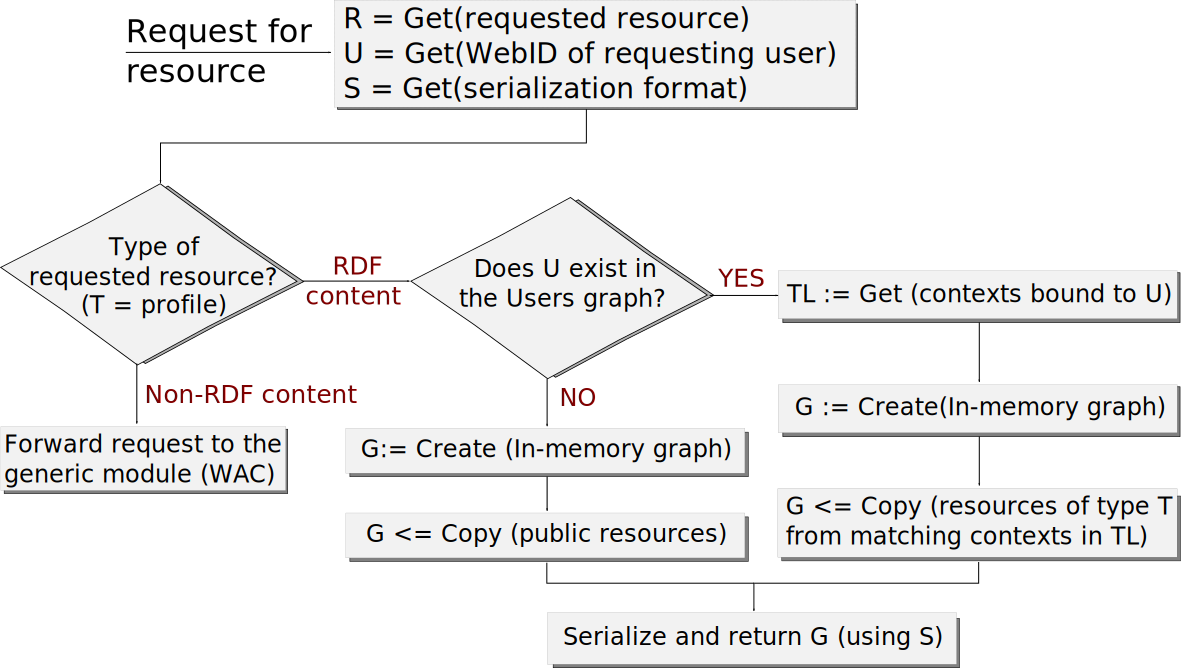
\includegraphics[width=270px]{img/algorithm-matching.pdf}
        \caption{Algorithme d'appariement contextuel.}
        \label{fig:context_matching_fr}
  \end{center}
\end{figure}

%The information contained in the \textit{Request} includes the type of the requested resource (T), the WebID of the requester (U) and the data serialization format (S) for the response (e.g. Turtle, RDF/XML, N3, etc.). At this point, we assume that the requesting user has already been authenticated at the moment of the request. If the user has not been authenticated, only the public view of the requested resource is returned.\\
Les informations contenues dans la demande inclut le type de la ressource demandée (T), le WebID du demandeur (U) et le format de sérialisation de données (S) pour la réponse (par exemple, Turtle, RDF / XML, N3, etc). À ce stade, nous supposons que l'utilisateur demandeur a déjà été authentifié au moment de la demande. Si l'utilisateur n'a pas été authentifié, seule la vue publique de la ressource demandée est renvoyée.\\


%The following step of the algorithm is to lookup the requester in the graph of users belonging to the resource owner. If there is no match, the requester receives only the public view of the requested resource. Otherwise, all contexts assigned to the requester's WebID are extracted, and a list of all contexts URIs (TL) is created.\\
L'étape suivante de l'algorithme est de rechercher le demandeur dans le graphique des utilisateurs appartenant au propriétaire de la ressource. Si aucune correspondance n'est trouvée, le demandeur ne reçoit que la vue publique de la ressource demandée. Sinon, tous les contextes affectés au WebID du demandeur sont extraites, et une liste de tous les contextes URI (TL) est crée.\\


%The next step is to create a temporary, in-memory graph (G), to store only the resources matching the requester's access policies. This graph will only be used during the processing of the algorithm, to hold the contents of the reply.\\
L'étape suivante consiste à créer un graphe temporaire en mémoire (G), afin de conserver uniquement les ressources correspondant à la politique d'accès du demandeur. Ce graphe ne sera utilisé que pendant le traitement de l'algorithme, afin de maintenir le contenu de la réponse.\\


%Once the graph has been created, it is time to copy all resources belonging to the list of contexts (TL), and which correspond to the type of the request (e.g. a profile, a wall, a conversation, etc.).\\
Une fois que le graphe a été créé, il est temps de copier toutes les ressources appartenant à la liste des contextes (TL), et qui correspondent au type de la demande (par exemple, un profil, un mur, une conversation, etc).\\


%Finally, the graph (G) is serialized in the requested format (S) before being returned to the requesting user (U). As soon as the contents of (G) have been sent through HTTP(S), the graph is destroyed and memory is freed.
Enfin, le graphe (G) est mis en forme sur la base de la sérialisation demandée (S) avant d'être renvoyé à l'utilisateur demandeur (U). Dès que le contenu de (G) a été envoyé via HTTP(S), le graphe est détruit et la mémoire est libérée.

\addcontentsline{toc}{subsection}{Le moteur de la surveillance des relations}
\subsection*{Le moteur de la surveillance des relations}
%The \textit{Relationship Monitor} engine (RM) is tasked to analyse the dynamicity of relationships between two given users, in order to either provide notifications for potential privacy issues that may arise when disclosing information, or it may even modify existing access control policies for incoming requests (if so configured). The RM applies to two distinct types of actions. First, for assigning context labels when disclosing information, and second for handling a request for a resource.\\
Le moteur de surveillance des relations (Relationship Monitor - RM) est chargé d'analyser le caractère dynamique des relations entre les deux utilisateurs donnés, afin de fournir soit des notifications pour les éventuels problèmes de la vie privée qui peuvent surgir lors de la divulgation d'information, ou il peut même modifier les politiques de contrôle d'accès existants pour les requêtes entrantes (s'il est configuré pour). Le RM s'applique à deux types distincts d'actions. Tout d'abord, pour attribuer des étiquettes de contexte lors de la divulgation d'informations, et la seconde pour le traitement d'une demande de ressource.\\


%When a user intends to limit the audience for some of his/her private information (e.g. religious views, sexual orientation, etc.), he/she can assign one or more context labels to the information that is to be protected, as well as to the audience in order to indicate who can access the information. During this labelling process, the RM analyses user interaction data from the Relationship History database (Figure~\ref{fig:acs_architecture}), corresponding to the selected audience. Typical examples of user interactions include sharing a picture within a specific context (i.e. \verb+#closefriends+), explicitly changing a user's proximity level, excluding a user from a given context (without permanently removing him/her) when sharing a resource, the number of times users exchange messages (as a function of time), etc.\\
Quand un utilisateur a l'intention de limiter l'audience de certaines de ses informations personnelles (par exemple, opinions religieuses, l'orientation sexuelle, etc), il peut assigner une ou plusieurs étiquettes de contexte à l'information qui doit être protégée, ainsi que pour le public afin d'indiquer qui peut accéder à l'information. Au cours de ce processus d'étiquetage, la RM analyse les données d'interaction de l'utilisateur à partir d'un historique des relations (Relationship History database - Figure~\ref{fig:acs_architecture_fr}), correspondant à l'auditoire sélectionné. Des exemples typiques d'interactions entre les utilisateurs comprennent le partage d'une image dans un contexte spécifique (par exemple \verb+#closefriends+), changer explicitement le niveau de proximité d'un utilisateur, exclure un utilisateur à partir d'un contexte donné (sans l'enlever définitivement) lors du partage d'une ressource, combien de fois les utilisateurs échangent des messages (en fonction du temps), etc.\\


%Based on the interactions in Relationship History database, the RM may alert the user (i.e. provide visual indications) to a possible change in their relationship. For instance, a warning message may appear if the resource owner is in the process of assigning a context label (which corresponds to a specific proximity level) to a user which is in a more distant proximity level.\\
Basé sur les interactions dans le historique des relations, le RM peut alerter l'utilisateur (par exemple fournir des indications visuelles) à un éventuel changement dans leur relation. Par exemple, un message d'avertissement peut apparaître si le propriétaire de la ressource est en cours d'attribution d'une étiquette de contexte (ce qui correspond à un niveau de proximité spécifique) à un utilisateur qui se trouve dans un niveau de proximité plus lointain.\\


%The algorithm behing the RM's decision making process can be seen in Figure~\ref{fig:algorithm_rme}.\\
L'algorithme derriere le processus de prise de décision de la RM peut être vu dans la Figure~\ref{fig:algorithm_rme_fr}.\\

\begin{figure}[h]
  \begin{center}
    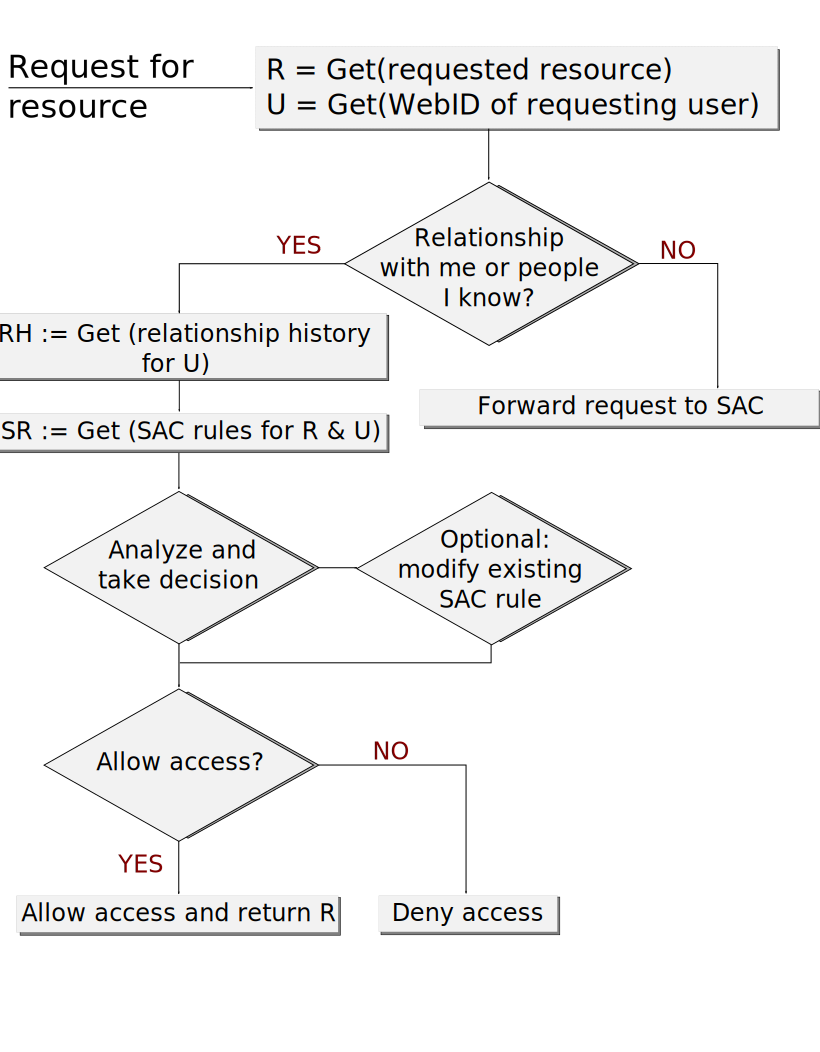
\includegraphics[width=270px]{img/algorithm-rme.pdf}
        \caption{Le processus de la prise de décision du RM.}
        \label{fig:algorithm_rme_fr}
  \end{center}
\end{figure}

%The information contained in the \textit{Request} includes the requested resource (R) and the WebID of the requester (U). At this point, we also assume that the requesting user has already been authenticated at the moment of the request. If the user has not been authenticated, the process will consider the user to be \textit{undetermined} (i.e. anyone with public access).\\
Les informations contenues dans la demande comprend la ressource demandée (R) et le WebID du demandeur (U). À ce stade, nous supposons également que l'utilisateur demandeur a déjà été authentifié au moment de la demande. Si l'utilisateur n'a pas été authentifié, le processus considèrent que l'utilisateur soit indéterminée (i.e. à toute personne ayant accès public).\\


%The following step is to decide if the user in question has any relationships with the resource owner or people known by the resource owner. This step is achieved by querying the Relationship History database to find occurrences of interactions between the requester and the resource owner, or by searching if the requester is friends with the resource owner or one of the resource owner's friends.\\
L'étape suivante consiste à décider si l'utilisateur en question a des relations avec le propriétaire de la ressource ou des personnes connues par le propriétaire de la ressource. Cette étape est effectuée en interrogeant la base de données contenant l'historique des relations pour trouver les occurrences d'interactions entre le demandeur et le propriétaire de la ressource, ou en recherchant si le demandeur est ami avec le propriétaire de la ressource ou l'un des amis du propriétaire de la ressource.\\


%If the two users have previously interacted with each other, a graph (RH) containing the list of interactions will be created. Additionally, all static access control rules corresponding to the user (U) and resource (R) will be imported from the policies database and stored in a new graph (SR).\\
Si les deux utilisateurs partagent un historique des relations, un graphe (RH) contenant la liste des interactions sera créé. De plus, toutes les règles statiques de contrôle d'accès correspondant à l'utilisateur (U) et ressources (R) seront importées à partir de la base de données des politiques et stockés dans un nouveau graphe (SR).\\


%Next, based on the the contents of (RH) and (SR), the system will analyse an decide on a course of action. If the data from (RH) is found to be heavily conflicting with the rules in (SR) and if the RM engine is operating in \textit{unsupervised mode}, the system may optionally modify existing SAC rules. For example, if the requester was deemed to have changed proximity distance either through an evolution of his/her relationship towards the resource owner, or because the resource owner explicitly modified the user's proximity distance, the system may be able to reflect this change in the SAC rules.\\
Ensuite, basé sur le contenu de (RH) et (SR), le système va analyser et décider d'un plan d'action. Si les données de (RH) se trouve être fortement contradictoires avec les règles (SR) et si le moteur RM fonctionne en mode sans surveillance, le système peut éventuellement modifier les règles SAC existants. Par exemple, si le demandeur est réputé avoir changé sa distance de proximité, soit par une évolution de sa relation envers le propriétaire des ressources, soit parce que le propriétaire de la ressource a explicitement modifié la distance de proximité de l'utilisateur, le système peut être en mesure de refléter ce changement dans le règles SAC.\\


%Once the final decision is made, the RM engine will either grant access or deny access to the requested resource.
Une fois que la décision finale est prise, le moteur RM va accorder ou refuser l'accès à la ressource demandée.


\addcontentsline{toc}{section}{Validation de nos travaux de recherche}
\section*{Validation de nos travaux de recherche}
%A truly decentralized social Web application, based on Semantic Web technologies, requires several key components. It must be able to offer decentralized user identity, secure authentication, semantic data storage, to apply Create-Read-Update-Delete (CRUD) operations to resources, to offer increased privacy through access control, and most importantly, to be interoperable with other applications in terms of data exchange (e.g. content sharing, messaging, activity notifications, etc.).
Une application Web véritablement décentralisée, basée sur les technologies du Web sémantique, nécessite plusieurs éléments clés. Elle doit être en mesure d'offrir une identité décentralisée pour l'utilisateur, d'offrir une authentification sécurisée, du stockage de données sémantique, appliquer des opérations Create-Read-Update-Delete (CRUD) aux ressources, d'offrir plus d'intimité grâce au contrôle d'accès, et surtout, d'être interopérable avec d'autres applications en termes d'échange de données (par exemple, le partage de contenu, la messagerie, les notifications d'activité, etc).

\addcontentsline{toc}{subsection}{MyProfile}
\subsection*{MyProfile}
%MyProfile project is a reflection of all efforts we have made over the course of this thesis. It intends to provide to users the privacy they deserve for the data they produce and own. It offers a unified user account, which centralizes the user's data and puts it under the user's control, and also on a device the user controls. It is a radical change from the \textit{walled gardens} of today's Web, where data are trapped in \textit{silos}.\\
Le projet de MyProfile est le reflet de tous les efforts que nous avons faits au cours de cette thèse. Il vise à fournir aux utilisateurs la la vie privée qu'ils méritent pour les données qu'ils produisent et détiennent. Il dispose d'un compte d'utilisateur unifiée, qui centralise les données de l'utilisateur et le met sous le contrôle de l'utilisateur, et également sur un dispositif appartenant à l'utilisateur. C'est un changement radical par rapport aux \textit{jardins clos} du Web d'aujourd'hui, où les données sont piégées dans des \textit{silos}.\\


%The platform also offers other services that do not require a local profile. Any user is able to \textit{view} his/her profile data in a friendlier and attractive way. While viewing the profile data, the platform displays the user's list of known people (i.e. friends), some basic information for each friend (e.g. full name, nickname, email, blog), as well as a text mention in case the relationship is bidirectional (i.e. "Has you as friend.").\\
La plate-forme propose également d'autres services qui ne nécessitent pas un profil local. N'importe quel utilisateur peut visualiser ses données de profil d'une manière conviviale et attrayante. Lors de l'affichage des données de profil, la plate-forme affiche la liste des utilisateurs de gens connus (i.e. amis), quelques informations de base pour chaque ami (par exemple nom, prénom, pseudo, email, blog), ainsi qu'une mention de texte au cas où la relation est bidirectionnelle (i.e. "vous a comme ami.»).\\


%Once authenticated, additional functionalities become available. For example, users can post messages to a public \textit{wall}, which is a common place for all users to write about news, events, social updates, etc. Users can also \textit{subscribe} to local services in order to have their own private wall, which is only available to their list of known people. Subscribing also allows users to send and receive private messages, as well as notifications when other users have posted something on their private wall.\\
Une fois authentifié, des fonctionnalités supplémentaires sont disponibles. Par exemple, les utilisateurs peuvent envoyer des messages sur un mur public, qui est un lieu commun pour tous les utilisateurs à écrire à propos de nouvelles, des événements sociaux, des mises à jour, etc. Les utilisateurs peuvent également s'abonner à des services locaux afin d'avoir leur propre mur privé, ce qui est disponible uniquement à leur liste de personnes connues. S'abonner permet également aux utilisateurs d'envoyer et de recevoir des messages privés, ainsi que des notifications lorsque d'autres utilisateurs ont posté quelque chose sur leur mur privé.\\

%The source code for MyProfile has been released under an MIT license (less restrictive compared to other open source licenses), and it is publicly available on GitHub under MyProfile\footnote{https://github.com/MyProfile/myprofile}. For portability and deployment reasons, the platform was mainly written in PHP and JavaScript. It relies on Virtuoso\footnote{http://virtuoso.openlinksw.com/} to facilitate RDF-triple storage and SPARQL queries for cached profiles. A running demo of MyProfile can be accessed at https://my-profile.eu/.
Le code source pour MyProfile a été publié sous une licence MIT (moins restrictive par rapport à d'autres licences open source), et il est accessible au public sur GitHub sous MyProfile\footnote{https://github.com/MyProfile/myprofile}. Pour des raisons de portabilité et de déploiement, la plate-forme a été principalement écrit en PHP et JavaScript. Elle s'appuie sur un système de stockage de triplets RDF basé sur Virtuoso\footnote{http://virtuoso.openlinksw.com/}, qui offre des requêtes SPARQL pour les profils mis en cache. Une démo fonctionnelle de MyProfile peut être consultée à https://my-profile.eu/.

\addcontentsline{toc}{subsection}{Authentification WebID}
\subsection*{Authentification WebID}
%WebID-TLS authentication plays a crucial role in MyProfile. On one hand it allows any authenticated user to post messages on walls or contact other people, regardless if they have a local account or not. On the other hand, local users that have been authenticated can also easily update their profiles, issue new certificates or manage their friends.\\
Authentification WebID-TLS joue un rôle crucial dans MyProfile. D'une part, il permet à tout utilisateur authentifié d'envoyer des messages sur les murs ou contacter d'autres personnes, peu importe si elles ont un compte local ou non. D'autre part, les utilisateurs locaux qui ont été authentifiés peuvent aussi facilement mettre à jour leurs profils, émettre de nouveaux certificats ou de gérer leurs amis.\\


%There exists two different WebID-TLS authentication approaches, either perform the WebID-TLS verification locally, or use a third party WebID-TLS authentication service. We have developed two libraries, written in PHP, which cover both approaches. The libraries have been released under the MIT license, and are publicly available on GitHub under WebIDauth\footnote{https://github.com/organizations/WebIDauth}. In the following subsections we will describe both libraries, as well as how the Web server must be configured to offer WebID-TLS authentication.
Il existe deux approches d'authentification WebID-TLS différentes. Ils peuvent soit effectuer la vérification WebID-TLS localement ({WebIDauth}) ou utiliser un autre service tiers d'authentification WebID-TLS (WebIDDelegatedAuth). Nous avons développé deux bibliothèques, écrites en PHP, qui couvrent les deux approches. Les bibliothèques ont été publiées sous la licence MIT, et sont accessibles au public sur GitHub sous WebIDauth\footnote{https://github.com/organizations/WebIDauth}. Dans les paragraphes qui suivent, nous allons décrire les deux bibliothèques.

\subsubsection*{WebIDauth}
%Local authentication can be achieved by relying on \textit{WebIDauth}, a PHP library implementing WebID-TLS. Its particularity resides in the fact that it allows users to request a \textit{verbose} authentication process, which is useful when debugging a faulty certificate or a user profile.\\
L'authentification locale peut être réalisée en s'appuyant sur WebIDauth, une bibliothèque PHP qui implémente WebID-TLS. Sa particularité réside dans le fait qu'il permet aux utilisateurs de demander un processus d'authentification verbeux, ce qui est utile lors du débogage d'un certificat défectueux ou un profil d'utilisateur.\\


%WebIDauth can operate in two modes. In the first mode, its task is to perform WebID-TLS authentication and simply return either \textit{true} or \textit{false}, depending whether the user was successfully authenticated or not. This mode is intended to be used as an authentication method for a local application, usually coupled with a user session. However, operating in this mode also implies configuring the Web server to run over HTTPS, adding to the expenses of hosting the local application by having to buy a server certificate.\\
WebIDauth peut fonctionner dans deux modes. Dans le premier mode, sa tâche consiste à effectuer une authentification WebID-TLS et il suffit de retourner \textit{Vrai} ou \textit{Faux}, selon si l'utilisateur a été authentifié avec succès ou non. Ce mode est prévu pour être utilisé comme un procédé d'authentification pour une application locale, généralement associée à une session d'utilisateur. Cependant, fonctionnant dans ce mode implique également la configuration du serveur Web pour exécuter via HTTPS, en ajoutant aux dépenses de l'hébergement de l'application locale la nécessité acheter un certificat de serveur.\\


%In the second operation mode, WebIDauth can be used as a Relying Party, a third-party service that provides a WebID-TLS authentication endpoint for Web applications that cannot perform the authentication process themselves. There are several advantages to using a Relying Party service. For instance, it drastically reduces the complexity of having to set up the Web server to allow WebID-TLS authentication. Additionally, the service provider (local application) may not require HTTPS, therefore the owners do not need to pay for a server certificate.
Dans le deuxième mode de fonctionnement, WebIDauth peut être utilisé comme un service tiers qui fournit un point d'accès authentification WebID-TLS pour les applications Web qui ne peuvent pas effectuer le processus d'authentification eux-mêmes (essentiellement un RP). Dans le deuxième mode de fonctionnement, WebIDauth peut être utilisé comme un service tiers qui fournit un point d'accès authentification WebID-TLS pour les applications Web qui ne peuvent pas effectuer le processus d'authentification eux-mêmes (essentiellement un RP). Il ya plusieurs avantages à utiliser un service tiers. Par exemple, il réduit considérablement la complexité d'avoir à configurer le serveur Web pour permettre l'authentification WebID-TLS. En outre, le prestataire de service (application locale) n'a pas à exiger HTTPS, donc les propriétaires n'ont pas besoin de payer pour un certificat de serveur.


\subsubsection*{WebIDDelegatedAuth}
%Delegated WebID-TLS authentication is the process of relying on a third-party service to perform the authentication, and then redirect the user back to the Service Provider, as seen Section~\ref{sec:webid-tls_delegated_auth}. This is currently the default operation mode for MyProfile. The WebIDDelegatedAuth library was created so that Service Providers can offer WebID-TLS authentication in case they are not capable of offering local authentication, or they do not operate over HTTPS. Let us now explore each step of the process.\\
L'authentification WebID-TLS délégué est le processus de s'appuyer sur un service tiers pour effectuer l'authentification, puis rediriger l'utilisateur vers le fournisseur de services. Ce n'est pas le mode de fonctionnement par défaut pour MyProfile. La bibliothèque WebIDDelegatedAuth a été crée afin que les fournisseurs de services puissent offrir une authentification WebID-TLS dans le cas où ils ne sont pas capables d'offrir une authentification locale, ou ils ne fonctionnent pas via HTTPS. Examinons maintenant chaque étape du processus.\\


%First, the user clicks a login button on the Service Provider (i.e. https://my-profile.eu) and is redirected to the Relying Party (i.e. https://auth.my-profile.eu), thus triggering the authentication process. The Service Provider also appends a variable to the redirection URI, containing the Service Provider's URI: \textit{https://auth.my-profile.eu/?authreqissuer=https://my-profile.eu}.\\
Tout d'abord, l'utilisateur clique sur un bouton de connexion sur le fournisseur de services (i.e. https://my-profile.eu) et est redirigé vers le RP (i.e. https://auth.my-profile.eu), déclenchant ainsi le processus d'authentification. Le fournisseur de service ajoute également une variable à l'URI de redirection, contenant l'URI du fournisseur de services: \textit{https://auth.my-profile.eu/?authreqissuer=https://my-profile.eu}.\\


%Next, the Relying Party uses WebIDauth to perform WebID-TLS authentication. If the user has been successfully authenticated, the Relying Party prepares the redirection request, appending additional arguments to the redirection URI, namely the \textit{webid}, \textit{ts}, \textit{referrer} and \textit{sig}, with the following meanings:
Ensuite, le RP utilise la bibliothèque WebIDauth pour effectuer une authentification WebID-TLS locale. Si l'utilisateur a été authentifié avec succès, le RP prépare la demande de redirection, en ajoutant des arguments supplémentaires à l'URI de redirection, comme le \textit{webid}, \textit{ts}, \textit{referrer} et \textit{sig}, qui ont les significations suivantes:

\begin{itemize}
\item \verb+webid+ - WebID: https://my-profile.eu/people/barry/card\#me.
\item \verb+ts+ - horodatage: 2013-05-22CEST16\%3A54\%3A04\%2B02\%3A00
\item \verb+referrer+ - https://auth.my-profile.eu
\item \verb+sig+ - signature: hR5cv9gPn.....MxBbSdq7f.
\end{itemize}

\addcontentsline{toc}{subsection}{Espaces de données personnelles basés sur RWW.I/O}
\subsection*{Espaces de données personnelles basés sur RWW.I/O}
%Offering individual data stores is an important aspect of any decentralized social application, as users must be allowed to choose where they want to host their data, as well as to have complete control over the privacy settings that apply to that data. If possible, data stores should be hosted by devices to which the user has physical access. However, for performance reasons, data stores may be located on third party servers, if users are not concerned by privacy issues.\\
Offrant des espaces individuels de données est un aspect important de toute application sociale décentralisée. Les utilisateurs doivent être autorisés à choisir où ils veulent héberger leurs données, ainsi que d'avoir un contrôle complet sur les paramètres de confidentialité qui s'appliquent à ces données. Si possible, les espaces données doivent être hébergés sur des dispositifs auxquels l'utilisateur a un accès physique. Cependant, pour des raisons de performances, les espaces de données peuvent être situés sur des serveurs tiers, si les utilisateurs ne sont pas concernés par les questions de confidentialité.\\


%RWW.I/O stands for \textit{Read-Write-Web Input/Output} and it operates under the assumption that users require a personal data store, where different applications can store data about and for the user, and where data are equally available between applications. The advantage is that different applications can reuse the same data, to offer different functionalities. For example, a contact management application can pull data from the user's profile and modify it at the user's request. The modifications are instantly reflected in the user's profile the next time someone accesses the profile.\\
RWW.I/O signifie \textit{Read-Write-Web Input/Output} et fonctionne sous l'hypothèse que les utilisateurs ont besoin d'un espace de données à caractère personnel, où les différentes applications peuvent stocker des données sur et pour l'utilisateur, et pour lesquels des données sont également disponibles entre les applications. L'avantage est que les différentes applications peuvent réutiliser les mêmes données, afin d'offrir des fonctionnalités différentes. Par exemple, une application de gestion de contacts peut extraire des données à partir du profil de l'utilisateur et de le modifier à la demande de l'utilisateur. Les modifications sont immédiatement reflétées dans le profil de l'utilisateur la prochaine fois que quelqu'un accède au profil.\\


%Being invited to work with Sir Tim Berners-Lee on access control for the the Semantic Web at the Massachusetts Institute of Technology, has allowed me to develop a Linked Data personal data store platform that implements the WAC~\cite{hollenbach2009using} ontology. The platform supports full Create-Read-Update-Delete (CRUD) operations, following the REST standards. Documents and directories can be created by performing HTTP requests such as POST, PUT and MKCOL (i.e. new directories), following the requirements we presented at the beginning of the chapter. The \textit{Content-Type} HTTP header plays a central role to interpreting the requests and deciding whether to store data as triples or as binary files. As RWW.I/O is not intended to be a fully-fledged cloud service, only a handful of content types are supported (e.g. text/turtle, text/n3, application/rdf+xml, application/json, text/html, image/jpg, image/png).\\
Être invité à travailler avec Sir Tim Berners-Lee sur le contrôle d'accès pour le Web Sémantique au Massachusetts Institute of Technology, m'a permis de commencer le développement de RWW.I/O tandis que la mise en œuvre de l'ontologie WAC. La plate-forme prend en charge les opérations complètes Create-Read-Update-Delete (CRUD), suivant le standard REST. Documents et répertoires peuvent être créés en effectuant des requêtes HTTP tels que POST, PUT et MKCOL (nouveaux répertoires), suivant les besoins, nous avons présenté au début de ce document. L'en-tête HTTP \textit{Content-Type} joue un rôle central pour interpréter les demandes et décider de stocker des données comme des triplets ou sous forme de fichiers binaires. Comme RWW.I/O n'est pas destiné à être un service de cloud à part entière, seule une poignée de types de contenu sont pris en charge (e.g. text/turtle, text/n3, application/rdf+xml, application/json, text/html, image/jpg, image/png).\\


%The code is written in PHP, Python and JavaScript, and is publicly available under an MIT license on Github at
Le code est écrit en PHP, Python et JavaScript, et est accessible au public sous une licence MIT sur Github à \textbf{rww.io}\footnote{https://github.com/deiu/rww.io}.


\addcontentsline{toc}{section}{Conclusions}
\section*{Conclusions}
%At the beginning of this thesis we set out to identify which are the key components that would help us achieve true data ownership and interoperability for the next-gen social Web. While decentralisation is the most important factor of the equation, our model would not work unless true interoperability is achieved. For this reason, we decided to use Semantic Web technologies, as they provide true interoperability as well as helping represent data in a way that cannot be confusing or misleading.\\
Au début de cette thèse, nous avons commencé à identifier quels sont les éléments clés qui pourraient nous aider à parvenir à une véritable propriété des données et l'interopérabilité pour le Web social de prochaine génération. Si la décentralisation est le facteur le plus important de l'équation, notre modèle ne fonctionne que si une véritable interopérabilité est obtenue. Pour cette raison, nous avons décidé d'utiliser les technologies du Web sémantique, car elles offrent une véritable interopérabilité ainsi que d'aider représenter des données d'une manière qui ne peut pas prêter à confusion ou induire en erreur.\\


%During this thesis we have contributed to three different research topics, ranging from decentralized identity to authentication and access control. To validate our contributions to the research world, we have participated in the standardization process of WebID and WebID-TLS at the World Wide Web Consortium (W3C), which has allowed us to obtain immediate feedback from experts all around the world.\\
Au cours de cette thèse, nous avons contribué à trois thèmes de recherche différents, allant de l'identité décentralisée  à l'authentification et au contrôle d'accès. Pour valider nos contributions dans le monde de la recherche, nous avons participé au processus de standardisation du WebID et WebID-TLS au sein du World Wide Web Consortium (W3C), qui nous a permis d'obtenir des commentaires immédiats de la part des experts du monde entier.\\


%Furthermore, we were able to translate our research results into working services and applications, which are currently used as base references for work in this domain. All our implementation efforts consist of open source software, publicly available on GitHub with an MIT license.
Enfin, nous avons réussi à matérialiser nos résultats de recherche en services et applications qui sont actuellement utilisés comme références de base pour les travaux dans ce domaine. Tous nos efforts de mise en œuvre consistent en des logiciels open source, disponibles au public sur GitHub avec une licence MIT.

\clearpage


% Appendix - Examples


\addcontentsline{toc}{chapter}{Appendix - Examples}
\chapter*{Appendix - Examples}
\markboth{\MakeUppercase{Appendix - Examples}}{}

\begin{example}[h]
\begin{minted}{apache}
<VirtualHost my-profile.eu:443>
        ServerName my-profile.eu
        ServerAdmin admin@my-profile.eu

        DocumentRoot /var/www/myprofile
        <Directory />
                Options FollowSymLinks
                AllowOverride All
        </Directory>

        <Directory /var/www/myprofile/>
                Options -Indexes FollowSymLinks MultiViews
                AllowOverride All
                Order allow,deny
                allow from all
        </Directory>

        # Enable/Disable SSL for this virtual host.
        SSLEngine on

        # Log
        LogLevel info
        ErrorLog ${APACHE_LOG_DIR}/error-ssl.log		
        CustomLog ${APACHE_LOG_DIR}/ssl_access.log combined

        # SECURITY - only accept TLS
        SSLProtocol All -SSLv2
        
        SSLCertificateFile    /etc/ssl/certs/my-profile.eu.crt
        SSLCertificateKeyFile /etc/ssl/private/my-profile.key
        SSLCertificateChainFile /etc/apache2/cert/gandiCA.pem

        # MSIE 7 and newer should be able to use keepalive
        BrowserMatch "MSIE [17-9]" ssl-unclean-shutdown
</VirtualHost>
\end{minted}
\caption{Web server configuration file for MyProfile.}
\label{app:mp_conf}
\end{example}

\newpage
\begin{example}[h]
\begin{minted}{apache}
<VirtualHost auth.my-profile.eu:443>
        ServerName auth.my-profile.eu
        ServerAdmin admin@my-profile.eu

        DocumentRoot /var/www/auth
        <Directory />
                Options FollowSymLinks
                AllowOverride All
        </Directory>
        <Directory /var/www/auth/>
                Options Indexes FollowSymLinks MultiViews
                AllowOverride All
                Order allow,deny
                allow from all
        </Directory>

        # Possible values include: debug, info, notice, warn, error, crit,
        # alert, emerg.
        LogLevel debug 
        
        ErrorLog ${APACHE_LOG_DIR}/error-auth.log
        CustomLog ${APACHE_LOG_DIR}/ssl_access-auth.log combined

        # SSL Engine Switch
        SSLEngine on

        # SECURITY
        # only accept TLS
        SSLProtocol All -SSLv2
        SSLInsecureRenegotiation on

        SSLCertificateFile    /etc/ssl/certs/auth.my-profile.eu.crt
        SSLCertificateKeyFile /etc/ssl/private/auth.my-profile.eu.key
        SSLCertificateChainFile /etc/ssl/certs/gandi-intermediate.pem

        SSLVerifyClient optional_no_ca
        SSLVerifyDepth 9
        SSLOptions +StdEnvVars +ExportCertData +OptRenegotiate

        # MSIE 7 and newer should be able to use keepalive
        BrowserMatch "MSIE [17-9]" ssl-unclean-shutdown
</VirtualHost>
\end{minted}
\caption{Web server configuration file for the Relying Party.}
\label{app:auth_conf}
\end{example}

\newpage
\begin{example}[h]
\begin{minted}{php}
<?php
require_once('WebIDDelegatedAuth/lib/Authentication.php');
$auth = new Authentication_Delegated();

if (!$auth->isAuthenticated()) { 
    echo $auth->authnDiagnostic;
    echo '<a href="https://auth.my-profile.eu/auth?authreqissuer=<SP URI>">';
    echo 'Click here to Login';
    echo '</a>';
} else { 
    echo 'Your have succesfully logged in!';
    print_r($auth);
}
\end{minted}
\caption{Authenticating with WebIDDelegatedAuth.}
\label{app:webiddelegatedauth}
\end{example}


% general bibliography
\addcontentsline{toc}{chapter}{Bibliography}
\bibliographystyle{plain}
\bibliography{thesis}

\end{document}